\documentclass[12pt,oneside]{report}

\usepackage[utf8]{inputenc}
\usepackage[backend=biber, sorting = none]{biblatex}

\addbibresource{./reference.bib}
% linktocpage shall be added to snippets.

% \usepackage{hyperref,theoremref}
% \hypersetup{
% 	colorlinks, 
% 	linkcolor={red!40!black}, 
% 	citecolor={blue!50!black},
% 	urlcolor={blue!80!black},
% 	linktocpage % Link table of content to the page instead of the title
% }

\usepackage{subfiles}
\usepackage{blindtext}
\usepackage{tikz}
\usetikzlibrary{cd}
\usetikzlibrary{positioning}

\usepackage{amssymb}
\usepackage[utf8]{inputenc}
\usepackage{mathtools}
\usepackage{titlesec}
\usepackage{amsthm}
\usepackage{thmtools}
\usepackage{amsmath}
\usepackage{graphicx}
\usepackage{titlesec}
\usepackage{xcolor}
\usepackage{multicol}
% \usepackage{hyperref}
\usepackage{import}
\usepackage{savetrees}

\usepackage{algorithm}
\usepackage{algpseudocode}
\usepackage[toc,page]{appendix}
\usepackage{listings}
\lstdefinestyle{cppstyle}{
    language=C++,
    basicstyle=\ttfamily\footnotesize,        % Small but readable font
    keywordstyle=\color{blue}\bfseries,       % Keywords in blue and bold
    stringstyle=\color{teal},                 % Strings in teal
    commentstyle=\color{gray}\itshape,        % Comments in italic gray
    morecomment=[l][\color{magenta}]{\#},     % Preprocessor directives in magenta
    numbers=left,                             % Line numbers on the left
    numberstyle=\tiny\color{gray},            % Small gray line numbers
    stepnumber=0,                             % Number every line
    frame=single,                             % Add a thin border around the code
    rulecolor=\color{black},                  % Border color
    tabsize=4,                                % Set tab width
    breaklines=true,                          % Enable line wrapping
    breakatwhitespace=true,                   % Break at spaces
    showspaces=false,                         % Hide space markers
    showstringspaces=false,                   % Hide spaces in strings
    captionpos=b,                             % Caption at bottom
    aboveskip=5pt,                            % Space before code block
    belowskip=5pt,                            % Space after code block
    backgroundcolor=\color{black!5},          % Light gray background
}

\lstdefinestyle{python}{
    language=Python,
    basicstyle=\ttfamily\footnotesize,        
    backgroundcolor=\color{black!5},    % Light gray background
    keywordstyle=\bfseries\color{blue}, % Bold blue keywords
    stringstyle=\color{teal},           % Teal strings
    commentstyle=\color{gray},          % Gray comments
    stepnumber=0,                             % Number every line
    frame=single,                             % Add a thin border around the code
    rulecolor=\color{black},                  % Border color
    tabsize=4,                                % Set tab width
    breaklines=true,                          % Enable line wrapping
    breakatwhitespace=true,                   % Break at spaces
    showspaces=false,                         % Hide space markers
    showstringspaces=false,                   % Hide spaces in strings
    captionpos=b,                             % Caption at bottom
    aboveskip=5pt,                            % Space before code block
    belowskip=5pt,                            % Space after code block
    backgroundcolor=\color{black!5},          % Light gray background
}


\usepackage{float}
\usepackage{subcaption}
\newcommand{\dd}[1]{\mathrm{d}#1}


\newtheorem{thm}{Theorem}[chapter]
\newtheorem{lemma}[thm]{Lemma}
\newtheorem{coro}[thm]{Corollary}
\newtheorem{prop}[thm]{Proposition}
\theoremstyle{definition}
\newtheorem{defn}[thm]{Definition}

\theoremstyle{definition}
\newtheorem{axiom}[thm]{Axiom}
\newtheorem{observation}[thm]{Observation}

\theoremstyle{remark}
\newtheorem{remark}[thm]{Observatio}
\newtheorem{hypothesis}[thm]{Coniectura}
\newtheorem{example}[thm]{Example}
\newtheorem{exmp}[thm]{Example}
\newtheorem{exampple}{Example}

\renewcommand\emptyset{\varnothing}
\renewcommand\mod{\text{ mod }}
%TODO mayby proof environment shall have more margin
% \renewenvironment{proof}{\vspace{0.4cm}\noindent\small{\emph{Demonstratio.}}}{\qed\vspace{0.4cm}}
% \renewenvironment{proof}{{\bfseries\emph{Demonstratio.}}}{\qed}
\renewcommand\qedsymbol{Q.E.D.}
% \renewcommand{\chaptername}{Caput}
% \renewcommand{\contentsname}{Index Capitum} % Index Capitum 
% \renewcommand{\emph}[1]{\textbf{\textit{#1}}}
\renewcommand{\ker}[1]{\operatorname{Ker}{#1}}

%\DeclareMathOperator{\ker}{Ker}

% New Commands
\newcommand{\bb}[1]{\mathbb{#1}} %TODO add this line to nvim snippets
\newcommand{\orb}[2]{\text{Orb}_{#1}({#2})}
\newcommand{\stab}[2]{\text{Stab}_{#1}({#2})}
\newcommand{\im}[1]{\text{im}{\ #1}}
\newcommand{\se}[2]{\text{send}_{#1}({#2})}
\newcommand{\be}{b_\text{eff}}
% \renewcommand{\L}{L_{\lambda}(x)}

% project specific macros
% m stands for maximum
\newcommand{\mx}{\overline{x}}

\date{7 March, 2025}
\title{Quantifying Chaos}
\author{Luc Dixon, Yuhao Han, Logan Hinkley}

\usepackage[y4project,fancyhdr,hyperref,colour]{edmaths}
\renewcommand{\L}{L_{\lambda}}
\flushbottom

\begin{document}
\maketitle

\pagenumbering{roman}

\chapter*{Acknowledgements}
\addcontentsline{toc}{chapter}{Acknowledgements}
We sincerely thank our supervisor, Prof. Jacques Vanneste, without whose support and guidance this report would have been impossible.

\begin{abstract}
Chaos is a universal phenomenon observed in every aspect of the physical world. Examples include weather systems, celestial movements, demographic evolutions, and economic activities. 
The descriptions thereof often comprise of the adjective `unpredictable,' `disordered,' `entropic,' `confusing,' subject to chances, and, in summary, `chaotic.'
It may be of surprise that much more can be said to the even the simplest example.
In this report we will demonstrate there are rich, universal, and quantitative mathematical properties shared by all of these chaotic systems.

We begin by introducing examples of chaos and their defining characteristics. 
The intuitive descriptions of chaos, as will be shown, can be rigorously described by Lyapunov exponents and fractal dimensions.
After this, the iterative logistic map as a model of population is studied in detail, which exhibit an interesting behaviour of periodic bifurcations to chaos that is also observed among a large class of dynamical systems. 
The pinnacle of this report, presented in the last chapter, after developing some mathematically rigorous tools to study chaos, is the demonstrations of Feigenbaum's universal constants of bifurcation.
\end{abstract}
\declaration
\dedication{Musa mihi causas memora ...\\
	Muse, tell me the causes ...
}

\tableofcontents
\newpage
\pagenumbering{arabic}

% \addcontentsline{toc}{chapter}{Introduction}
\chapter*{Introduction}
\addcontentsline{toc}{chapter}{Introduction}
The Oxford English Dictionary definition of chaos is `utter confusion or disorder' \cite{OED}. 
In mathematics, this definition can be applied to the behaviours of \textit{dynamical systems}\footnote{A \emph{dynamical system} is described by the time-dependence of initial conditions for some function, e.g. a system of differential equations acting on a specific initial point.}. 
For a dynamical system, chaos can be summarised to be a sensitive dependence on initial conditions.
In the real world, this sensitivity is the cause of many limitations we face in modelling dynamical systems. For instance, we cannot reliably predict the weather past a certain number of days since any deviation from the exact measurements often results in a completely different outcome. The famous `butterfly effect'\footnote{“Does the flap of a butterfly's wings in Brazil set off a tornado in Texas?” - Edward Lorenz} is synonymous with this idea.

%An example of chaos that has been shown comes from the Lorenz system, which demonstrated different the impact different conditions had on the weather, highlighting the challenges in trying to predict the weather. The model for the Lorenz system is
%\begin{align*}
    %\frac{dx}{dt} &= \sigma (y-x), \\
    %\frac{dy}{dt} &= x(\rho -z)-y, \\
   % \frac{dz}{dt} &= xy-\beta z.
%\end{align*}
%When plotted over different initial conditions, the plots appear to possess different traits.
%\begin{figure}
    %\centering
    %\includegraphics[width=1\linewidth]%{figures/output.png}
    %\caption{Lorenz system with varying parameters where we can see varying orbits occurs that converge towards different attractors}
    %\label{fig:lorenz}
%\end{figure}
%From each plot, the attractors appear to be in a different location. In the plot for $\rho = 28$, trajectories appear to take a wide variety of unique paths. This is a sign that the system is chaotic under the specific initial conditions.
\begin{exampple}
    An iconic example of a chaotic dynamical system is the Lorenz system, a model of atmospheric conditions\cite{lorenz1963deterministic}, which demonstrates how nearby points can end up on drastically different trajectories. The Lorenz system is modelled by the system of differential equations:
    \begin{align}
        \frac{dx}{dt} = \sigma (y-x), \quad \frac{dy}{dt} = x(\rho -z)-y \quad\text{and} \quad \frac{dz}{dt} = xy-\beta z.
    \end{align}\label{lorenzequation}
The classic values of the parameters are $\sigma=10$, $\rho=28$ and $\beta=8/3$, for which the system appears chaotic. Indeed, taking two initial points within a small neighbourhood, their trajectories stray far away from each other. Due to the nature of the Lorenz system, this means that two points could occupy entirely different regions of space at the same instant of time. The trajectories of two initial points after some time are shown in Figure \ref{fig:lorenzrb}.
\begin{figure}
    \centering
    \includegraphics[width=0.8\linewidth]{Images/lorenz red blue.png}
    \caption{The Lorenz `attractor' for parameter values $\sigma=10$, $\rho=28$ and $\beta=8/3$, traced out by the standard initial point $(x,\ y,\ z)=(1.0,\ 1.0,\ 1.0)$ in black. The trajectories of the initial points $(x,\ y,\ z)=(1.1,\ 1.0,\ 1.1)$ and $(x,\ y,\ z)=(1.0,\ 1.1,\ 1.0)$ after $1,000$ iterations are shown in red and blue, respectively.}
    \label{fig:lorenzrb}
\end{figure}
This behaviour is a key characteristic in chaotic dynamical systems. Applied to weather systems, suppose you are trying to model the whereabouts of particles in the air over time; it could be the case that only absolutely perfect measurements of the surrounding environment would give you a reliable prediction; this is, of course, unrealistic.
\end{exampple}
%There is no way to avoid the unpredictability of chaos. Instead, we
It is in our interest to find properties of chaotic systems that give an idea of their general behaviour; this is what it means to quantify chaos. Throughout this report, we will introduce chaotic systems and investigate methods that allow us to find quantifiable properties within them. 

In particular, we will look at: the Lyapunov exponent, which will show how sensitive a system is to its initial conditions, allowing us to determine whether or not a system is chaotic; attractors and their fractal dimension, telling us how a system approaches a set of points in phase space; the logistic map, a subtly complex system that showcases chaos, which will be our go-to example in many cases; and Feigenbaum's universal constants, numbers that reappear throughout a wide class of chaotic systems. Each of these topics will call for their own particular definitions of chaos, which vary in rigour. For that reason, we will investigate the simpler topics first and introduce the more rigorous definitions as they are needed.

Chaotic systems lend themselves to intricate plots of both their trajectories and their investigable properties. Throughout this report, we will use computer code to generate these plots as well as to make numerical and symbolic calculations and tables of their results. 

While most of our theorems and definitions come from standard literature on dynamical systems, all proofs, numerics, and figures are original unless otherwise stated.

\chapter{Lyapunov Exponents}
\section{Definitions and Numerical Computations of Lyapunov Exponents}

One of the key defining properties of chaos in dynamical systems is that small perturbations\footnote{A `small perturbation' of an initial point means to take a new point that is very close to the original.} in the initial conditions lead to large differences over time.
With the assumption that the distance of nearby points increases exponentially, the following simplistic formula for the dynamical system of an iterative map $F$ can be deduced
\begin{align}\label{eq:lyapunov_exponent}
    \left|F^n(x_0+\epsilon)-F^n(x_0)\right| \sim \epsilon e^{n \lambda}, \text{ as } n \rightarrow \infty,
\end{align}
where $\lambda$ is the \emph{Lyapunov exponent} \cite{nonlinear_system}\cite{lyapunov}, $x_0$ is the point at discrete time $0$, and $F^n$ denotes composition of $F$ $n$ times.

A positive $\lambda$ means nearby points of $x_0$ will move away from it as time progresses, and a negative $\lambda$ means nearby points will converge to it.
The absolute value of $\lambda$ represents the rate of divergence or convergence. 

It should be clear from this that the Lyapunov exponent will play an important role throughout this report; it is a component of dynamical systems which will dictate chaotic behaviour.

The existence of such $\lambda$ is not obvious, the analytical evaluation of $\lambda$ is often hopeless, and the assumption seems very questionable.
However, if acquiescing in such a formula, $\lambda$ can be calculated numerically, giving important insights into the dynamical system. 

Assuming that $\epsilon e^{n \lambda} \to 0$ and $\epsilon$ is small, \eqref{eq:lyapunov_exponent} becomes
$$
\epsilon \left| \frac{dF^n(x_0)}{dx} \right| \sim \epsilon e^{n \lambda} \text{ as } n \rightarrow \infty.
$$
Taking the logarithm,
\begin{align}
    \lambda 
    &= \lim_{n \to \infty}\left(\frac{1}{n}\ln{\left|\frac{dF^n(x_0)}{dx}\right|}\right)  \\
    &= \lim_{N \to \infty}\left\{\frac{1}{N}\sum_{n=0}^{N-1}\ln{|F'(x_n)|}\right\}  \label{eq:lambda},
\end{align}
where in the last step $F'$ is the derivative of $F$ respective to $x$, and we labelled the points $x_1 = F(x_0), x_2 = F(x_1), \dots$ and applied the chain rule.
All of the numerical calculations of Lyapunov exponents in this report will use \eqref{eq:lambda}.

Equation \eqref{eq:lambda} fails to make sense at the points $x$ where $F'(x) = 0$.
Such points are called \emph{superstability} points, and the Lyapunov exponents of which are defined as $- \infty$.

The following are some examples of calculating Lyapunov exponents.

\begin{exmp}
	A classical example of chaotic system is generated by the iteration of the tent map, which is defined by
    \begin{align}
        F(r, x)= 
        \begin{cases}
            r x, & \text{ if } x \in [0,1/2) \\
            r (1-x), & \text{ if } x \in [1/2,1]
        \end{cases} \label{eq:tent}
    \end{align}
    where $r$ is a parameter.
	The Lyapunov exponent at $0$ is $\ln r$, which is negative if $r < 1$ and positive otherwise.
	The higher subfigure of Figure \ref{fig:lyapunov_tent} is the \textit{bifurcation diagram} of the tent map, which shows how the long-term trajectories of some initial $x_0$ change as we vary the parameter $r$. 
	It is obtained by selecting $1,000$ equally spaced $r \in [0,2]$, and for each $r$ picking a random starting point $x_0$, iterating $x_0$ for $10,000$ times, ignoring the first $1,000$ iterations, and plotting the rest of the $9,000$ $ x_i$ as a faint blue dot at coordinate $(r, x_i)$. 
	There is a dramatic change in behaviour exactly at $r=1$, where the Lyapunov exponent changed from negative to positive.
    For $r < 1$ every $x_0$ converged to $0$, whereas afterwards the system shows an apparent chaotic behaviour by casting an interesting homogeneous shape of a double curved triangle. At $r = 2$, this system can be proved to be chaotic as will be shown in Example \ref{ex:logistic and tent}.

    \begin{figure}
        \centering
        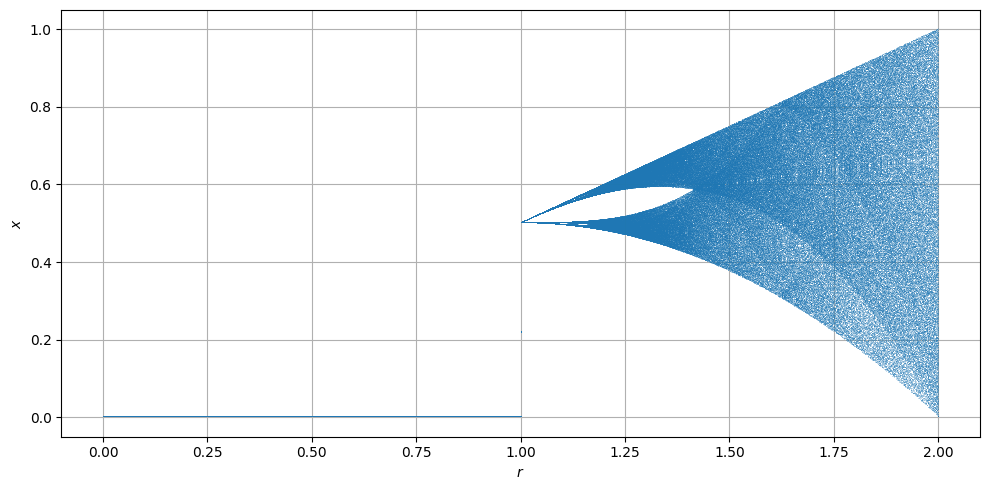
\includegraphics[width=\linewidth]{Bifurcation Images/bifurcation_tent.png}
        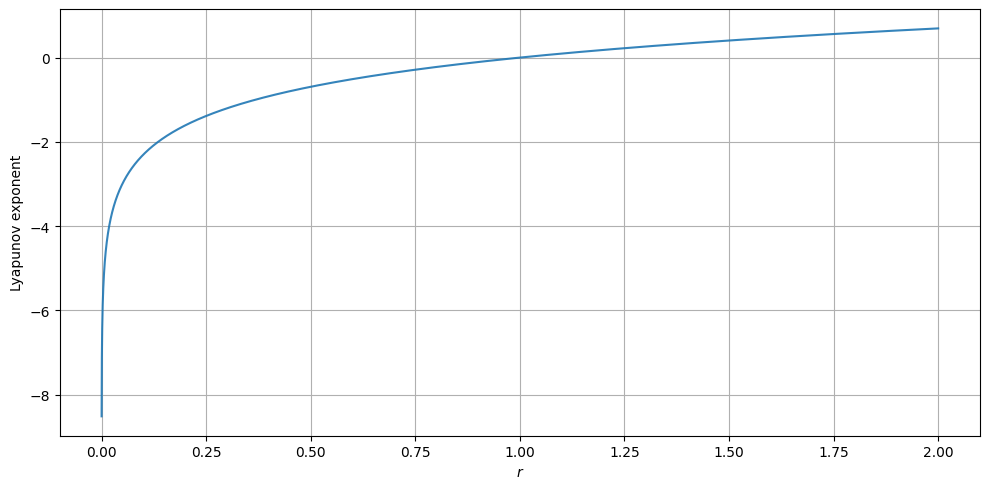
\includegraphics[width=\linewidth]{Bifurcation Images/lypaunov_tent.png}
        \caption{Bifurcation diagram (above) and Lyapunov exponent plot (below) for the tent map \eqref{eq:tent} over 10,000 iterations.}
        \label{fig:lyapunov_tent}
    \end{figure}
\end{exmp}

\begin{exmp}
	Similarly, consider the dynamical system depending on one parameter $r$ generated by the iterations of the map
    $F(r,x)=x^2+r$ where $x,r \in \mathbb{R}$.
	Unlike the case of the tent map, there is no simple closed form for the Lyapunov exponent, and computer simulations are required. 
	The bifurcation diagram and the Lyapunov exponent are shown in Figure \ref{fig:lyapunov_x^2}.
    \begin{figure}
        \centering
        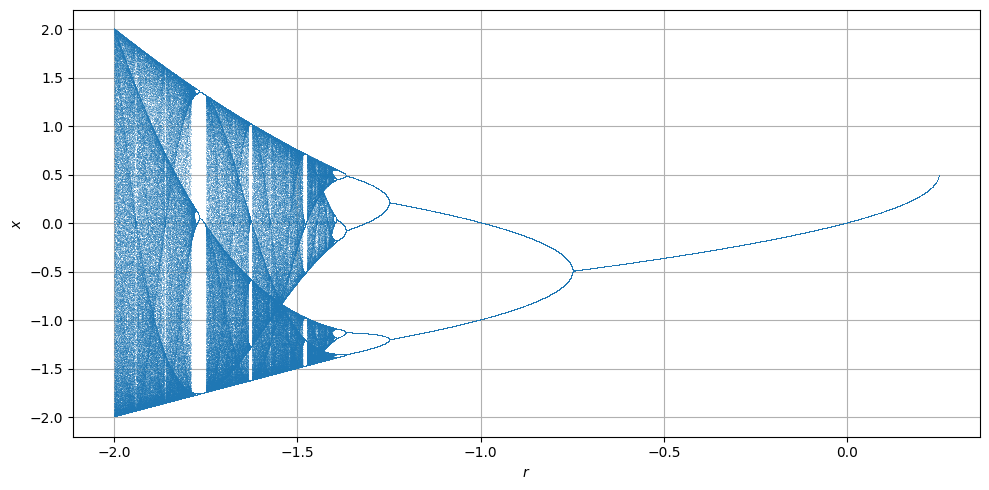
\includegraphics[width=1\linewidth]{Bifurcation Images/bifurcation_quadratic.png}
        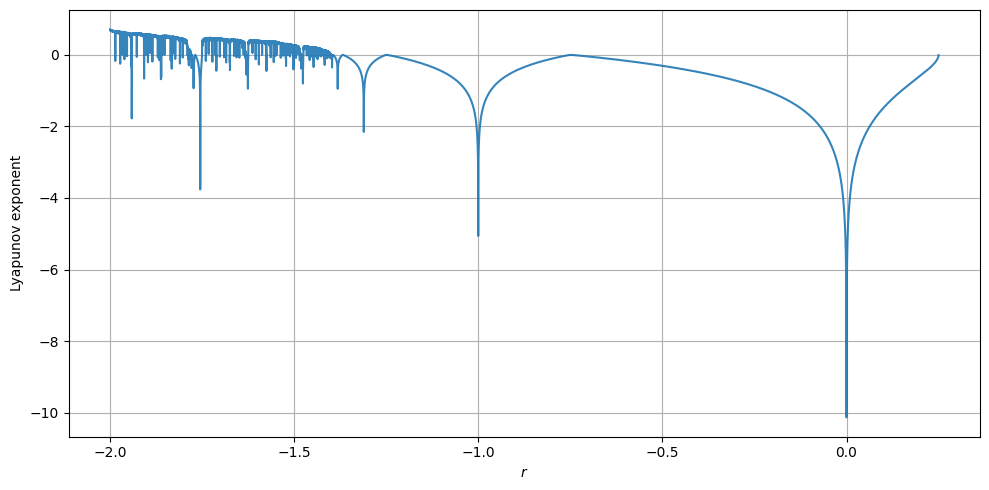
\includegraphics[width=1\linewidth]{Bifurcation Images/lypaunov_quadratic.png}
        \caption{Bifurcation diagram (above) and Lyapunov exponent plot (below) for the map $F(\lambda,x)=x^2+r$ over 50,000 iterations.}
        \label{fig:lyapunov_x^2}
    \end{figure}
	A very interesting phenomenon of period-doubling is apparent from the bifurcation diagram (which is studied in detail in Chapter \ref{chapter:bifurcation}).
	Similar to the tent map, regions where the Lyapunov exponent is negative correspond to distinct lines in the bifurcation diagram, while those with a positive Lyapunov exponent correspond to chaotic bands.
\end{exmp}


\section{Lyapunov Exponents for a Continuous Time Series}\label{LyapCts}

The Lyapunov exponents for continuous time dynamical systems in multiple dimensions exhibit very different behaviours compared to the simplistic one-dimensional discrete time dynamical systems discussed in the previous section. 
For continuous systems, we need to consider the complete spectrum of Lyapunov exponents. 
Given a continuous dynamical system in an $n$-dimensional phase space, we monitor the long-term evolution of an infinitely small $n$-sphere of initial conditions. 
It quantifies the average exponential growth or decay rates of perturbations in different directions in phase space. 
For an $n$-dimensional system, the Lyapunov spectrum consists of $n$ exponents, $\lambda_1 \geq \lambda_2 \geq \dots \geq \lambda_n$, which describe the system's behaviour in terms of expanding, neutral, and contracting directions. We can compute the spectra numerically.

Let's consider a continuous-time dynamical system defined by
$$
\dot{\mathbf{x}}(t) = \mathbf{f}(\mathbf{x}(t)),
$$
where $\mathbf{x}(t) \in \mathbb{R}^n$ is the state vector, and $\mathbf{f}$ is a smooth vector field and $t \geq0$ with initial conditions of $\mathbf{x}(0)=\mathbf{x_0}$. As with discrete systems, we may analyse the effects of initial perturbations on trajectories to determine whether they expand or contract. By using the trajectory $\mathbf{x}(t)$ and some nearby perturbation $\mathbf{y}=\delta\mathbf{x}(t)$, the linearised system becomes
$$
\dot{\mathbf{y}}(t) = \mathbf{J}(\mathbf{x}(t))\mathbf{y}(t),
$$
where $\mathbf{J}(\mathbf{x}(t))$ is the Jacobian matrix of $\mathbf{f}$ evaluated at $\mathbf{x}(t)$
$$
\mathbf{J}(\mathbf{x}(t)) = \frac{\partial \mathbf{f}}{\partial \mathbf{x}} \bigg|_{\mathbf{x}(t)}.
$$
The solution at the initial perturbation $\mathbf{y}(0)$ can be shown as $\mathbf{y}(t)=\mathbf{Y}(t)\mathbf{y}(0)$ where $\mathbf{Y}(t)$ is the fundamental solution, which satisfies
$$
\dot{\mathbf{Y}}=\mathbf{J}(\mathbf{x}(t))\mathbf{Y},
$$
where $\mathbf{Y}(0)$ is the identity matrix. Assume that $\det \mathbf{Y}(t)>0$, such that the initial perturbed trajectories never meet. The fundamental solution can be visually interpreted as an $n$-dimensional sphere of initial conditions evolving into an $n$-dimensional ellipsoid due to the locally deforming nature of the trajectories. The principal axis of the ellipsoid determines the Lyapunov vectors that grow or shrink at rates determined by the Lyapunov exponents. The principal axis are the directions along which the ellipsoid stretches or contracts the most where the Lyapunov vectors are the time-dependent vectors that align with the directions of the principal axis. Each Lyapunov vector $\mathbf{p}_i(t)$ stretches or contracts at a rate given by their corresponding Lyapunov exponent $\lambda_i$. The Lyapunov vectors are given as
$$
\mathbf{p}_i(t)=\mathbf{Y}(t)\xi_i(t),
$$
where $\xi_i(t)$ are the eigenvectors of $\sqrt{\mathbf{Y}^T\mathbf{Y}}$. Since the Lyapunov exponent measures the distance in the rate of growth or decay between the perturbations, we need to compute the length of the Lyapunov vector. Thus we take the norm of the principal axis. Using the same logic as for a discrete system, the $i$th Lyapunov exponent \cite{OED} is 
\begin{align}
    \lambda_i=\lim_{t \to \infty}\frac{1}{t}\ln ||\mathbf{p}_i(t)||.  \label{eq:lyapunov_cont} 
\end{align}

The Lyapunov exponents describe the long-term average exponential growth rates of perturbations in different directions or the $i$-th principal axis of the ellipsoid. A positive exponent ($\lambda_i > 0$) indicates expansion in the corresponding direction. A zero exponent ($\lambda_i = 0$) indicates a neutral direction, such as along the flow of a trajectory. A negative exponent ($\lambda_i < 0$) indicates contraction in the corresponding direction.

Note that we can also solve for the $i$-th Lyapunov exponent $\lambda_i$ using $\log_2,$
\begin{align}
    \lambda_i = \lim_{t \to \infty} \frac{1}{t} \log_2 ||\mathbf{p}_i(t)||, \label{eq:continuous}
\end{align}
in order to show that the ellipsoid grows with a rate of $2^{\lambda_1t}$. The area of the ellipsoid is defined by the first two principal axes $2^{(\lambda_1+\lambda_2)t}$, the volume by the first three, $2^{(\lambda_1+\lambda_2+\lambda_3)t},$ and so on. \cite{continuouslyapunov}

For dissipative systems (systems that release energy instead of retaining it), the sum of the Lyapunov exponents is negative, indicating that the volume of the ellipsoid contracts over time.

In three dimensions, the sum of all the Lyapunov exponents is equivalent to the trace of the system's corresponding Jacobian matrix. 
In order for the system to be chaotic, only one of the individual exponents needs to be positive.
The possible Lyapunov spectra and the corresponding attractors are: $(+,0,-)$, which signifies chaotic behaviour; $(0,0,-)$, which tells us that the system will demonstrate quasi-periodic behaviour;
$(0,-,-)$, which corresponds to the presence of a limit cycle or periodic behaviour; and $(-,-,-)$ , which tells us that there is a stable fixed point. 
The sum of the Lyapunov exponents equals the time-averaged divergence of the phase space velocity. 
The value indicates the divergence of the flow and is the fractional rate of the volume expansion or contraction of the system, but for a conservative or Hamiltonian system, this sum is zero. 
For dissipative systems, this sum is negative, ensuring that at least one exponent is negative. 
As a result, the long-term motion of trajectories converge to a limit set with zero volume, known as an attractor. 
While Lyapunov exponents are defined based on long-time averages, short trajectories may not fully capture the distinct behaviours associated with positive, zero, and negative exponents. \cite{continuouslyapunov}

% To compute the Lyapunov spectrum numerically, we start by linearising the system by solving for the Jacobian matrix $\mathbf{J}(\mathbf{x}(t))$ along the reference trajectory $\mathbf{x}(t)$. We then need to evolve the perturbation vectors. We need to initialize a set of $n$ orthonormal perturbation vectors $\{\mathbf{v}_1, \mathbf{v}_2, \dots, \mathbf{v}_n\}$ and evolve them using the linearised dynamics
% $$
% \dot{\mathbf{v}}_i(t) = \mathbf{J}(\mathbf{x}(t)) \mathbf{v}_i(t).
% $$
% Subsequently we need to use the Gram Schmidt reorthonormnalisation on the vector frame that we created in order to to maintain their independence and prevent numerical overflow. Then we can track the growth rates of the perturbation vectors and accumulate their logarithmic growth rates
% $$
% \sum_{i=1}^n \ln \|\mathbf{v}_i(t)\|.
% $$
% where the Lyapunov exponents are computed as the time-averaged logarithmic growth rates
% $$
% L_i = \lim_{t \to \infty} \frac{1}{t} \ln\frac{\|\mathbf{v}_i(t)\|}{\|\mathbf{v}_i(0)\|}.
% $$


\begin{exmp} An example of a continuous dynamical system is the Lorenz system \ref{lorenzequation} using the parameter values of $ \sigma = 10, \rho = 28 $ and $ \beta = 8/3$. Solving for the system's Jacobian allows for the use of $QR$ decomposition on the corresponding eigenvectors. After substituting the norm of these vectors and re-orthonormalising them, we can then obtain their average as we vary the time. \cite{OED}
\begin{figure}
    \centering
    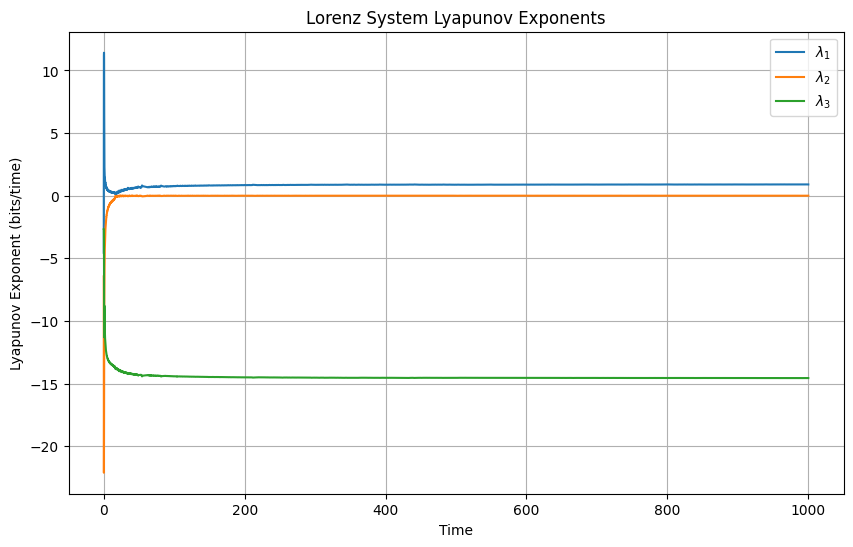
\includegraphics[width=1\linewidth]{Images/lorenz_lypunov.png}
    \caption{All values of $\lambda_i$ iterated over varying increasing time for the Lorenz system with parameter values of $\sigma = 10, \rho = 28$ and $\beta = 8/3$ with initial position of $(x,y,z)=(0.1,0.1,0.1)$. One exponent, $\lambda_1$ is shown to be greater than zero implying that at the conditions the system experiences chaos.}
    \label{fig:enter-label}
\end{figure}
As we iterate further in time, we get more accurate values for the different Lyapunov exponents, %$\lambda_i$
\begin{align*}
    \lambda_1 = 0.8973919196967531, \\
    \lambda_2 = 0.0000295072803878 ,\\
    \lambda_3 = -14.56408778526921,
\end{align*}
where $\lambda_1>0$, being positive, is responsible for the chaotic nature of the Lorenz system.
%which corresponds to the chaotic nature of the Lorenz system due to $\lambda_1>0$.
\end{exmp}
The first crucial step of this report is now complete; we have identified the key property of dynamical systems that attributes to chaos. We may now begin to investigate further quantifiable properties of chaotic dynamical systems; the Lyapunov exponent will reappear throughout this task due to its importance.
% Given a continuous dynamical system in an $n$-dimensional phase space, we monitor the long-term evolution of an infinitesimal $n$-sphere of initial conditions. The sphere will become an $n$-ellipsoid due to the locally deforming nature of the flow. The $i$th one-dimensional Lyapunov exponent is then defined in terms of the length of the ellipsoidal principal axis $p_i(t)$
% \begin{align}
%     L_i=\lim_{n \to \infty} \frac{1}{n}\log_2\frac{p_i(t)}{p_i(0)} \label{eq:continous}
% \end{align}
% where $L_i$ are the individual exponents. Thus the Lyapunov exponents are related to the expanding or contracting nature of different directions in phase space. Since the orientation of the ellipsoid changes continuously as it evolves, the directions associated with a given exponent vary in a complicated way through the attractor. One cannot, therefore, speak of a well-defined direction associated with a given exponent. From \eqref{eq:continous} we can see that the ellipsoid grows with a rate of $2^{L_1t}$. The area is defined by the first 2 principle axis $2^{(L_1+L_2)t}$, and the volume by the third$2^{(L_1+L_2+L_3)t}$. From this we can create a new definition for the spectrum of exponents, the sum of the first $j$ exponents is define by the long term exponential growth rate of a $j$-volume element. This will provide us with a basis for the spectra technique fro experimental data.

% Any continuous time dependent dynamicla system without a fixed point will have at least one zero exponent which links with the slowly changing magnitude of a principle axis  tangent to the flow

% In a three-dimensional continuous dissipative dynamical system the only possible spectra, and the attractors they describe, are as follows: $( + , 0 , - )$ , a strange attractor; $(0,0,-)$, a two-toms; $(0, - , -)$, a limit cycle; and $( - , - , - )$ , The sum of each individual exponents is the time-averaged divergence of the phase space velocity; hence any dissipative dynamical system will have at least one negative exponent, the sum of all of the exponents is negative, and the post transient motion of trajectories will occur on a zero volume limit set, an attractor. Since Lyapunov exponents involve long-time averaged behavior, the short segments of the trajectories shown in the figure cannot be expected to accurately characterize the positive, zero, and negative exponents; nevertheless, the three distinct types of behavior are clear.

% The Lyapunov spectrum is closely related to the fractional dimension of the associated strange attractor.
%--------------------------------------------------------------------------------------------------%

% \textbf{Show that the $p$-cycle $\{X_1, X_2, \dots, X_p\}$ of the continuously differentiable map $F: \mathbb{R} \to \mathbb{R}$ is stable if  
% \[
% | F'(X_1) F'(X_2) \dots F'(X_p)| < 1.
% \]
% This is a proof the textbook refers to a lot in the section and I dont know how to interpret it or include it.}


% Idea: If we have an initial condition $x_0$ which will generate our sequence for a distcete dynamical system to use discrete time, and a point nearby $x_0 + \epsilon_0$. Let $\epsilon_n$= separation of orbits from $x_0$ and orbit from $x_0 + \epsilon_0$

% If $|\epsilon_n| \sim |\epsilon_0|e^{n\lambda}$ is converging exponentially, $\lambda$ is they lyanopunov exponent
% -$\lambda>0$ means chaos
\chapter{Fractal Dimension}
%Chaotic systems, when visualised, often exhibit complex patterns due to their non-linear behaviour. These objects can loosely be defined as fractals\footnote{There are many definitions for what a fractal is. Mandelbrot defines them as (...)}, and we can measure how complicated one fractal is compared to another. Though our notion of chaos is not necessarily relevant in this section, fractal dimension will be used to measure the complexity of chaotic systems in further sections.%

%Fractal dimension can be summarised as the measure of an object's complexity or detail. Unlike the dimension of standard objects, fractal dimensions can take non-integer values. This allows objects in the same space to be compared in terms of how complicated their shape is. There are multiple ways to calculate or approximate an object's fractal dimension%
When studying dynamical systems that exhibit chaotic behaviour, we often choose to reduce them to a simpler form in order to obtain quantifiable properties. One key property we look for is \emph{fractal dimension}, which can be thought of as a set's complexity or detail. It can also be seen as a measure of how an object fills space at small scales. Formally, fractal dimension is an index of sets that characterises their complexity as a ratio of the change in detail to the change in scale \cite{mandelbrot1983fractal}. Unlike the values of dimension we are used to, fractal dimension can take non-integer values to distinguish between two objects that fill the same space but in different ways. For instance, a curve in $\mathbb{R}^2$ with fractal dimension close to one behaves much like a standard curve, while one with a fractal dimension close to two behaves more like a surface, e.g., a space-filling curve. Intuitively, we suspect that these distinctions are in close relation to the degree of sensitivity a system has to its initial conditions, which could imply a connection between fractal dimension and Lyapunov exponents. We can reduce a dynamical system to the set of points that its trajectories tend toward and find the fractal dimension of this set, giving us an idea of how the system behaves.

\section{Fractals}
There are many definitions for what a fractal really is, many of which are not rigorous and can only be applied in specific cases. Our definition will be that of Benoît Mandelbrot's.
\begin{defn}
    Let $X$ be a set. We say that $X$ is a fractal if its fractal dimension strictly exceeds its topological dimension. \cite{mandelbrot1983fractal}
\end{defn}
In this report, the term `topological dimension' will be equal to the standard Euclidean dimension we expect of objects. We have been vague in introducing the notion of non-integer values of dimension; this is because different methods of calculating fractal dimension are used depending on the context of the object. We will introduce these methods after the different contexts are clear.

\section{Self-Similarity and the Mass-Scaling Factor Method}
Our first context is one which is often used as a definition for fractals; that is, self-similar objects. Intuitively, \emph{self-similar} objects are those that are made up of smaller copies of themselves, such as a solid cube. We see a sense of self-similarity in nature, so fractals are often exemplified as, say, the branches of a tree. While fascinating, this notion of self-similarity will not be relevant in our case. We will see sets that are infinitely perfectly self-similar as they have been defined to be this way by an unbounded recursive construction.

While a little more abstract, the fractal dimensions of objects that exhibit self-similarity can be calculated in a simple way. The following method is motivated by translating our usual notions of an object's dimension to that of fractal dimension. 

\begin{prop} \label{MSF}
    (The mass-scaling factor method)
    \begin{enumerate}
        \item Say some self-similar object has a mass equal to one.
        \item Within the object, find a section that is an identical copy of the original.
        \item Comparing the copy to the original, work out the mass $m$ and scaling factor $s$ of the copy (this should be clear for simple self-similar shapes).
        \item Let $M=1/m$ and $S=1/s$. The fractal dimension $D$ of the object is then $S^D=M.$ Equivalently, $D=\log{_SM}$
    \end{enumerate}
\end{prop}
%\begin{defn}
    %The \textbf{scaling factor}, $S$ of a self-similar object is the ratio in size between itself and the `first' copy of itself.
%\end{defn}

%\begin{defn}
    %Suppose a self-similar object has `mass' equal to one. The \textbf{mass scaling factor}, $M$, of the object is the ratio between the masses of the object and the first copy of itself.
%\end{defn}
%\textbf{What do we mean by mass?}
%\begin{defn}
    %The \textbf{fractal dimension} of an object is the real number, $D$, such that $$S^D=M.$$ Equivalently, $$D=\log{_SM}$$
%\end{defn}
This definition of an object's dimension satisfies our usual methods of determining dimension; using elementary intuition, we can see that a straight line, a square, and a cube have fractal dimensions one, two, and three, respectively. In fact, the idea of dimension being a measure of how an object fills space has always been true for normal notions of dimension; scaling down a cube by some factor reduces its mass by that factor to the power of three, which is the dimension of the cube. As expected, this means they are not fractals due to the fractal dimension being equal to the topological dimension. However, what we have now is a distinction between, say, two curves in $\mathbb{R}^2$ or two surfaces in $\mathbb{R}^3$, where the higher fractal dimension points towards a more detailed structure.
%\begin{exmp}
    %The `Koch curve' is constructed by repeatedly adding triangular bumps to the centre-thirds of a line, starting with a straight line of unit length.
    
    %If we take a straight line and the Koch curve embedded in $\mathbb{R}^2$, both are continuous curves, so they are of the same dimension in the usual sense; however, we will see that the fractal dimensions are not equal due to the Koch curve being more complex. 
    %\begin{figure}
        %\centering
        %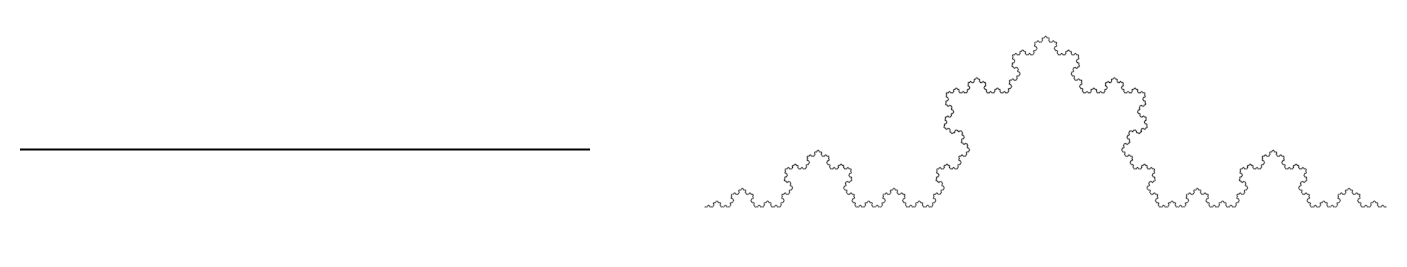
\includegraphics[width=0.8\linewidth]{Images/Koch.png}
        %\caption{Straight line and Koch Curve}
       % \label{fig:enter-label}
    %\end{figure}
    %Both are self-similar, since any cut of a line is similar to the line and the Koch curve splits into four identical copies of itself, each of which is scaled down in size by $1/3$. It is clear that, taking any cut of the straight line, say $1/a^{th}$ of it, gives a line of mass $1/a$, so we have that the line has a scaling factor equal to its mass-scaling factor, giving a fractal dimension of one, as we would expect. For the Koch curve, we have a scaling factor of $1/3$, since each copy of itself is $1/3^{rd}$ the length of the original and a mass-scaling factor of $1/4$, since we have four copies of this size. Therefore, we have that the fractal dimension of the Koch curve is given by the value of $D$ such that
    %$$\frac{1}{3}^D=\frac{1}{4},$$
    %equivalently, such that
    %$$3^D=4.$$
    %Therefore,
    %$$D=\log{_34}\approx1.26186.$$
    %This means that the Koch curve is a fractal, since its fractal dimension is strictly greater than its topological dimension which, being a curve in the plane, is one.
%\end{exmp}

\begin{exmp}
    The `Koch curve', pictured in Figure \ref{fig:Koch}, is constructed in the following way. Take a straight line segment embedded in $\mathbb{R}^2$ and remove the middle third and replace it with an `equilateral-triangle bump'. Note there are now four straight lines of length $1/3$ of the original. On each new straight line, add equilateral-triangle bumps to their middle thirds and repeat. At each stage, each quarter of the curve is an identical copy of the last version, scaled down by $1/3$.
    \begin{figure}
        \centering
        
\includegraphics[width=1\linewidth]{Images/Koch new.png}
        \caption{Construction of the Koch curve from a straight line, showing the first, second and fifth iterate. In blue are the sections of the Koch curve that are scaled copies of the iterate before it.}
        \label{fig:Koch}
    \end{figure}
    Let us follow the steps in Proposition \ref{MSF} to determine the fractal dimension of the Koch curve:
    \begin{enumerate}
        \item We say the Koch curve has mass and length one.
        \item Considering the curve after infinite iterates, each quarter of the curve is identical to the entire thing.
        \item Since each quarter of the curve is a copy of the original scaled down by $1/3$, one copy has mass $m=1/4$ and scaling factor $s=1/3$.
        \item We have $M=1/(1/4)=4$ and $S=1/(1/3)=3$, so the fractal dimension of the Koch curve is $D=\log_34\approx1.26186$
    \end{enumerate}
    Since the Koch curve is a continuous curve in $\mathbb{R}^2$, its topological dimension is one. Therefore, we have that the Koch curve is indeed a fractal, as its fractal dimension strictly exceeds its topological dimension.
\end{exmp}
%From the example above, we can see that we have a measurable value that will distinguish shapes based on their complexity. This will prove useful in chaos theory as knowing the fractal dimension of an object then allows us to talk about measures, which will be affected by the complexity of objects. The issue will be for objects that are not so simply defined and do not exhibit self-similarity. For this, we will need another method for calculating fractal dimension%.
We see here, a glimpse of what an object's fractal dimension is, with the restriction that our method only works in the case of perfect self-similarity. We have another method that does not depend on this property; however, the context in which it is used must first be introduced.
\section{Attractors and the Box-Counting Method}
We often want to look for the points that dynamical systems tend toward as time progresses. 
In our models, the existence and uniqueness theorem tells us that these points are deterministic in that fixed initial conditions will grant the same result every time. 
For stable systems, we can further say that some small perturbation of the initial conditions will not greatly affect the solution; this allows us to make strong predictions about how the system will evolve over time. 
With this in mind, we naturally arrive at the definition of an \emph{attractor}, the set of points in which a system evolves toward over time and then stays there forever. 
A key property of attractors is that they do not change under a small perturbation of initial conditions; trajectories of nearby points eventually fall into the same set of points. \cite{feldman2012chaos}

%\begin{defn}
    %An \textbf{attractor}, $\mathbf{X}  \in \mathbb{R}^n$, of an $n$-dimensional dynamical system, $F(\mathbf{x},t)$, is the set of points $\mathbf{x}_\infty\in\mathbb{R}^n$ that the trajectory of an initial point $\mathbf{x_0}$ tends toward $t\to\infty$.
    %$$\mathbf{X} := \{\mathbf{x}_\infty\in\mathbb{R}^n:F(\mathbf{x_0},t)\to\mathbf{x}_\infty \text{ as } t\to \infty\},$$
    %such that points in some small neighbourhood of %$\mathbf{x_0}$ will share the same attractor%.%
%\end{defn}%

%\begin{defn}
    %Let $F(\mathbf{x},t)$ be an $n$-dimensional dynamical system and $\mathbf{x_0}$ be some initial point. An \textbf{attractor}, $\mathbf{X}  \in \mathbb{R}^n$ of $\mathbf{x_0}$ is the set of points
    %$$\mathbf{X} := \{\mathbf{x}\in\mathbb{R}^n:F(\mathbf{x_0},t) = \mathbf{x}\},$$
    %such that the trajectories are dense near these points after some large $t$. Furthermore, points in some small neighbourhood of $\mathbf{x_0}$ share the same attractor.
%\end{defn}

%\begin{defn}
    %Let $F(\mathbf{x},t)$ be an $n$-dimensional dynamical system and $\mathbf{x_0}$ be some initial point. An \textbf{attractor}, $\mathbf{X}  \in \mathbb{R}^n$ of $\mathbf{x_0}$ is the set of points such that:
    %\begin{enumerate}
        %\item the trajectory remains dense in after some large number of iterations; and
        %\item points in some small neighborhood of $\mathbf{x_0}$ share the same attractor.
    %\end{enumerate}. 
%\end{defn}
%For simpler stable systems, we can find formulas for defining these sets by taking derivatives of the map $F$ and finding the stable points.

For stable systems, two types of attractors are: fixed points, a state of equilibrium; and limit cycles, a set of points that the system will eventually stay in, periodically, forever. 
%Since we have a set of distinct points in $\mathbb{R}^n$, we say these attractors are one-dimensional. 
%Small changes to the initial conditions will have a small effect on the attractors for stable systems. If we alter the parameters of a given system, we can see changes in stability as well as changes in the attractor type. 

%Given a system that is not stable, the trajectories may diverge. In a confined space, we have the example of a fluid mixing in a box, and we say that the attractor of this system is the whole three-dimensional space.
For chaotic systems, things are different. Since we have a strong sensitivity to initial conditions, even stable points can become unstable at the slightest perturbation due to the existence of a positive Lyapunov exponent. This means we cannot define the set so easily since a minor change to one initial point could greatly affect its outcome over time. This being said, we may not have complete divergence, since we can plot the trajectories after a high number of iterations and still see a distinct set. Furthermore, zooming in to these attractors, we see that they can take the form of fractals. 

These properties have coined the term `strange' attractors since they paradoxically show convergence of a system that seems to never settle down. Thus the term \emph{strange attractor} describes attractors that have a fractal structure and are those of dynamical systems that observe a sensitive dependence on initial conditions \cite{feldman2012chaos}. To better understand strange attractors, a staple example is the Hénon map, a simplified section of the famous Lorenz system \cite{nonlinear_system}.
\begin{exmp}
    We define the Hénon map, which acts on points $(x,y)\in \mathbb{R}^2$, as the two-dimensional discrete-time dynamical system,
\begin{equation}
    x_{n+1} = 1 - a x_n^2 + y_n, \quad y_{n+1} = b x_n.   
\end{equation}\label{Henonequation}
The classic parameters are $a=1.4$ and $b=0.3$, with which the map is chaotic. Plotting the trajectory of the initial point $(0,0)$ gives us a prime example of a strange attractor.
    \begin{figure}
        \centering
        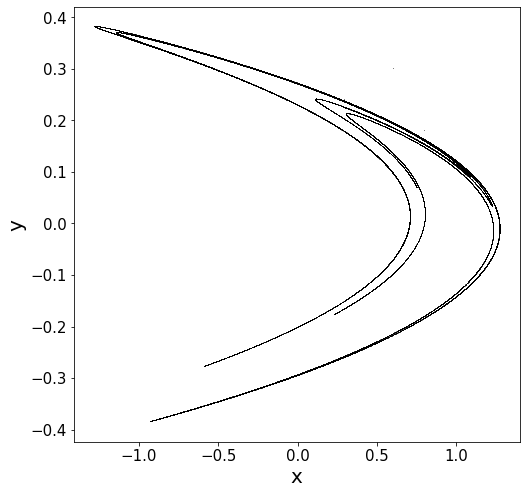
\includegraphics[width=0.4\linewidth]{Images/Henon attractor.png}
        \caption{$100,000$ iterations of the Hénon map with initial point $(x_0, y_0)=(0,0)$.}
        \label{fig:Henon1}
    \end{figure}
    We see the set of points this system attains as the nested curves in Figure \ref{fig:Henon1}. It is important to understand these curves are made up of distinct points, given by each iteration of the Hénon map, and these points are by no means following the curves continuously; we see that the 95th through 99th iterations\footnote{Choosing the 95th through 99th iterations was completely arbitrary in the interest of a diagram that represented the point well. Almost any iterations would have shown the sensitive dependence on initial conditions.} are far apart from each other and follow no obvious pattern. Changing the initial conditions by a small amount, the attractor remains similar, but these same iterations appear in drastically different positions on it, alluding to the chaotic nature of this system. This behaviour can be seen in Figure \ref{fig:Henon2}.
    \begin{figure}
        \centering
        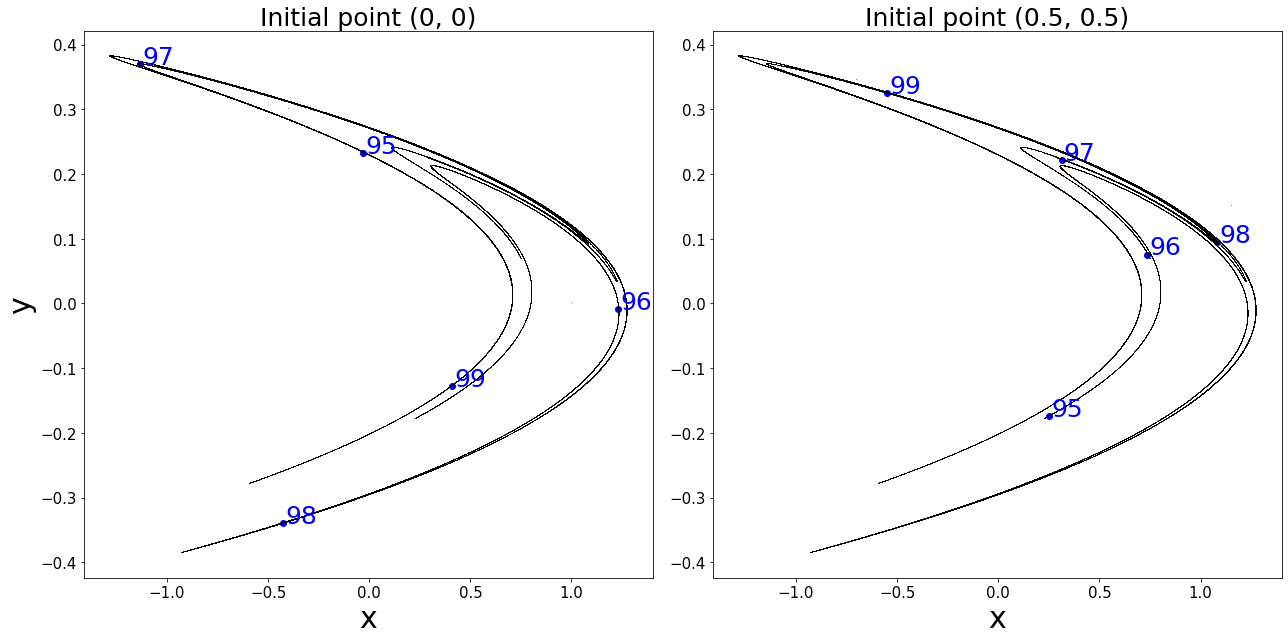
\includegraphics[width=0.75\linewidth]{Images/Henon attractor with labels.png}
        \caption{The Hénon attractor, generated from two different initial points, $(x_0,y_0) = (0,0)$ and $(x_0',y_0') = (0.5,0.5)$. The attractor is identical for both initial points while the system itself appears to be chaotic due to the iterates following drastically different trajectories.}
        \label{fig:Henon2}
    \end{figure}
    The fact that a similar attracting set exists for both initial points indicates this is an attractor by definition.
    Zooming into a section of it will show more self-similar curve, as shown in Figure \ref{fig:Henon3}, is another evidence of it being a strange attractor. 
    \begin{figure}
        \centering
        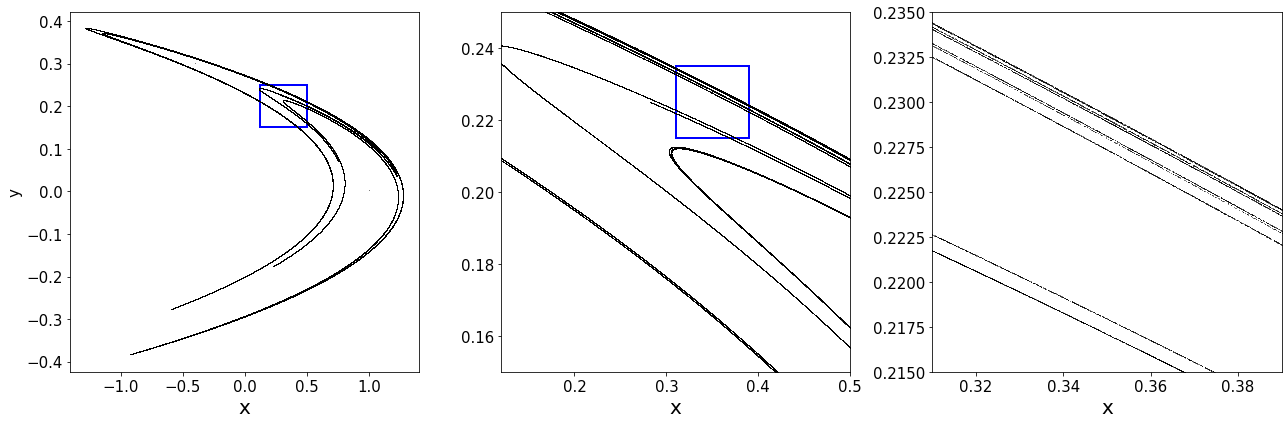
\includegraphics[width=1\linewidth]{Images/henon zoom.png}
        \caption{Zooming in to the blue boxes on the Hénon attractor to see the fractal structure of the object.}
        \label{fig:Henon3}
    \end{figure}
    Since the attractor has a fractal structure and its system has a sensitive dependence on initial conditions, we conclude that this is indeed a strange attractor.
\end{exmp}
From this example, it is clear that the mass-scaling factor method of determining fractal dimension will no longer be of use, since we cannot simply find a smaller version of the Hénon map inside itself, let alone determine its mass-scaling factor. However, the idea of how the attractor fills space will motivate a new method for approximating the value.

Motivated by the need for a universal method for calculating fractal dimension, the following method can be used to approximate the fractal dimension of any object in some subset of $\mathbb{R}^n$. The idea is, given some fractal object, we measure the amount of space it fills as we zoom into its structure. We do this by overlaying a grid of $n$-dimensional boxes over the object and counting how many boxes it is contained in. We then decrease the size of the boxes and count again, repeating this process a number of times. With the results, we plot the logarithms of the number of boxes against the size of the boxes and take the slope of best fit to be the fractal dimension. Explicitly, we have a formula
\begin{equation}
    D = \lim_{\epsilon \to 0} \frac{\log N(\epsilon)}{\log(1/\epsilon)},
\end{equation}\label{boxcountingD}
where $\epsilon$ is the size of each box (length of one side of each $n$-cube) and $N(\epsilon)$ is the number of boxes that the object is contained in for each $\epsilon$. For complicated objects, the best way to do this is by use of computer code that will do this whole process to a strong level of accuracy. It must be noted that Formula \ref{boxcountingD} may not be valid in practice since, in Python, it is only realistic to plot a finite number of points of the attractor. Therefore, we must be careful to fashion code that suits the attractor we are working with, or else the box-count can `bottom-out' once the boxes become too small, giving a skewed gradient. With this in mind, we return to the previous example to calculate the fractal dimension of the Hénon attractor by the box-counting method.
\begin{exmp}\label{henonboxex}
    Using Python, we calculate the fractal dimension of the Hénon attractor by following the box-counting method. The code overlays a grid of boxes over the fractal and counts the number of boxes that contain it as the box size decreases. In Figure \ref{fig:Henon4}, we see some blue boxes that contain the attractor as their size decreases.
    \begin{figure}
        \centering
        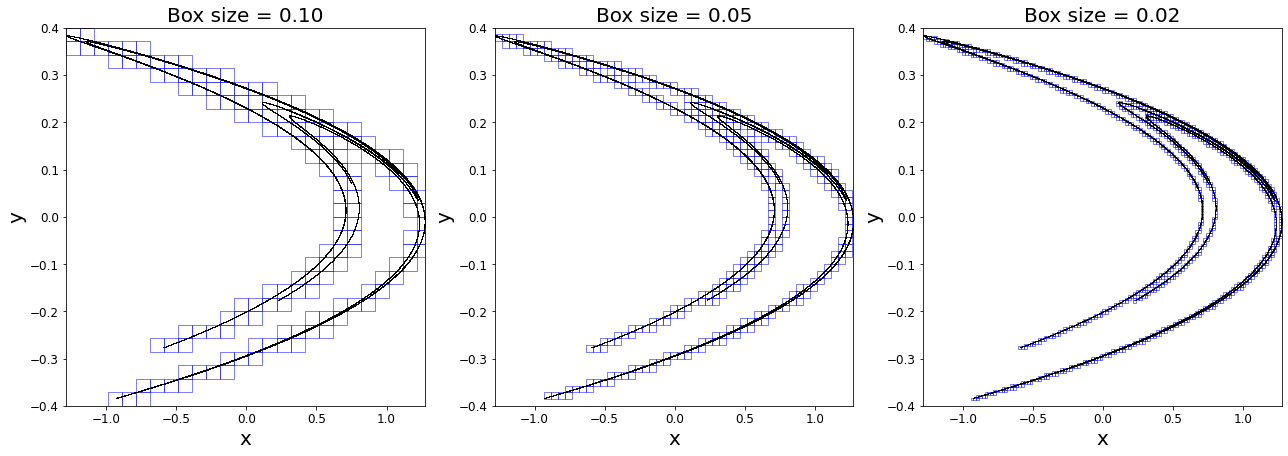
\includegraphics[width=1\linewidth]{Images/Henon boxes.png}
        \caption{Blue squares are those from the grid that contain at least one iterate of the Hénon attractor after $10,000,000$ iterations, using initial point $(0,0)$. The first $10,000$ iterates are discarded to remove any `dust' for accuracy.}
        \label{fig:Henon4}
    \end{figure}
    The code then plots $\log (N(\epsilon))$ against $\log (1/\epsilon)$ for many values of $\epsilon$ and finds the line of best fit through the points on the plot. The gradient of the line is then calculated to achieve a value for $D$. This is all given in Figure \ref{fig:Henon5}.
    \begin{figure}
        \centering
        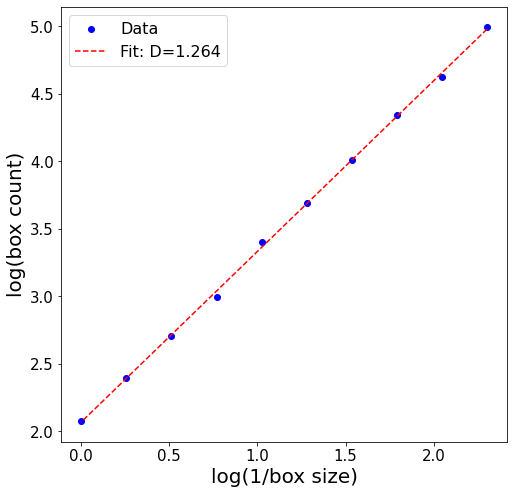
\includegraphics[width=0.5\linewidth]{Images/henon loglog.png}
        \caption{$\log (N(\epsilon))$ as a function of $\log(1/\epsilon)$ for ten values of $\epsilon$ and the line of best fit through the data points which has gradient equal to the fractal dimension of the Hénon attractor.}
        \label{fig:Henon5}
    \end{figure}
    From the gradient of the line, we get a value of $D\approx1.264$, which is our fractal dimension of the Hénon attractor by the box-counting method. The code written for this example is shown in Appendix \ref{boxalg}.
\end{exmp}
With this, we have a more versatile method for calculating the fractal dimension of a fractal object in $\mathbb{R}^n$. We find one more method for fractal dimension calculation by returning to Section \ref{LyapCts}.


\section{The Kaplan–Yorke Conjecture}

The Lyapunov spectrum, as discussed in Section \ref{LyapCts}, is closely related to the fractal dimension of the attractor. The Kaplan–Yorke conjecture uses Lyapunov exponents to deduce the dimension of an attractor within a dynamical system.
%In order to quantify the complexity of chaotic attractors, which often exhibit fractal structure, Lyapunov exponents can help provide information about the system's dynamics, while fractal dimension characterises the geometry of the attractor.
The conjecture is able to link these two concepts together, which is based on the idea that the sum of Lyapunov exponents relates to the expansion and contraction rates of phase space volumes. 
The fractal dimension is then estimated by balancing the cumulative expansion (positive Lyapunov exponents) against the cumulative contraction (negative Lyapunov exponents). 
Let us arrange the Lyapunov exponents from largest to smallest such that $\lambda_1 \geq \lambda_2 \geq \dots \geq \lambda_n$. Let $k$ thus be the largest index in which
\begin{align}
    \sum_{i=1}^k \lambda_i\geq 0 \quad\quad \text{ and } \quad \quad \sum_{i=1}^{k+1} \lambda_i <0 \label{eq:criteria}
\end{align}

We then have the Kaplan-Yorke dimension \cite{Peitgen1992}, defined as
\begin{align}
    D = k + \frac{\sum_{i=1}^k \lambda_i}{|\lambda_{k+1}|},\label{Kaplan-Yorke}
\end{align} 
where $k$ is the largest integer such that $\sum_{i=1}^k \lambda_i \geq 0,$ which provides an estimate of the fractal dimension. We return once more to the example of the Hénon Map to calculate its Kaplan-Yorke dimension.

\begin{exmp}
    When we compute the Lyapunov exponent for the Hénon Map \eqref{Henonequation} using Section \ref{LyapCts}, we attain the values approximated by the graphs in Figure \ref{fig:LyaHen}.
    \begin{figure}
        \centering
        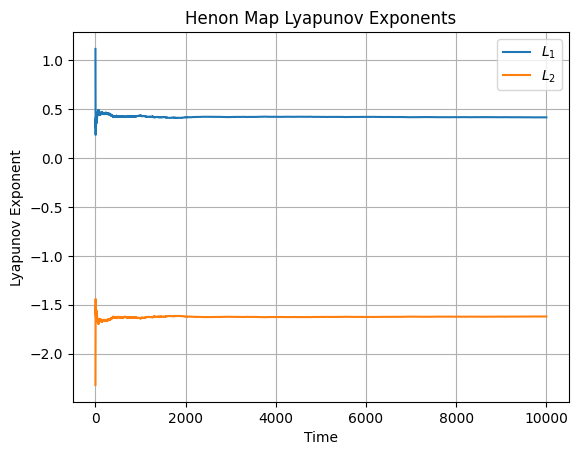
\includegraphics[width=0.8\linewidth]{Bifurcation Images/lyapunov_henon.png}
        \caption{Lyapunov exponents for the Hénon Map with initial conditions of $(x,y)=(0.1,0.1)$ where $a=1.4$ and $b=0.3$. The exponent $\lambda_1$ after several iterations of time is seen to be greater than 0 implying that the system is chaotic under the initial conditions.}
        \label{fig:LyaHen}
    \end{figure}
    The Lyapunov exponents for the Hénon map were computed to be 
    \begin{align*}
        \lambda_1 &= 0.41762663136121125, \\
        \lambda_2 &= -1.6215994356871315,
    \end{align*}
     when we used \eqref{eq:lyapunov_cont}. However if we use \eqref{eq:continuous}, we get the exponents to be 
    \begin{align*}
        \lambda_1 &= 0.6025078700079933, \\
        \lambda_2 &= -2.339473464174202.
    \end{align*}
    From \eqref{eq:criteria}, we can observe that our value for $k$ must be 1. Thus when we substitute these values into \eqref{Kaplan-Yorke},
    \begin{align}
        D &= 1 + \frac{\sum_{i=1}^1 \lambda_i}{|\lambda_{2}|} \\
        &=1 + \frac{0.6025078700079933}{|-2.339473464174202|} \\
        &=1.257539946.
    \end{align}
    This gives us that the fractal dimension of the Hénon attractor by the Kaplan–Yorke conjecture is $D=1.257\dots$, which aligns very closely to the result found in Example \ref{henonboxex}. This provides evidence for the conjecture's validity and shows there could be some connection between fractal dimension and Lyapunov exponents, as suspected.

We now have a range of methods to calculate fractal dimension, giving an index of fractals distinguished by their small-scale complexity. 
This complexity and these fractal shapes are seen throughout nature as a characteristic of what we consider to be a natural-looking shape\footnote{“Clouds are not spheres, mountains are not cones, coastlines are not circles, and bark is not smooth, nor does lightning travel in a straight line.”
― Benoît Mandelbrot \cite{mandelbrot1983fractal}}.
Noticing this, computer image generation uses fractals to create shapes that look natural, such as mountain ranges, plants, and coastlines. Without fractals, we could do our best to draw the detailed ridge of a mountain range from a given distance away, but the detail would not remain as we move closer. Fractals allow us to generate this detail to any scale; which, in the interest of realistic simulation, makes for a much better representation of such objects. The fractals we use depend on what we are trying to model; mountain ranges, plants, and coastlines all have different ranges of fractal dimensions that best represent their real-life structure. \cite{Haeseler2012}
\end{exmp}

%\section{Fractal Dimension Implications}
%For chaotic dynamical systems, we can now quantify the dimension of the attractors with values that better represent the strange structure they can have. These values give us an idea of the properties of the system itself.\\

%First, the higher the fractal dimension, the more an attractor of a system fills the space it occupies. In an $n$-dimensional subset of $\mathbb{R}^n$, this means that an attractor with a fractal dimension close to $n$ will be associated with a system that has a higher number of effective degrees of freedom.
%In particular, suppose we are working in some subset of $\mathbb{R}^2$. We have, on one extreme, that the attractor of the system is a single fixed point, where we would have a zero-dimensional attractor. On the other extreme, the attractor is the whole space, two-dimensional. A one-dimensional attractor would be one that takes the form of a smooth continuous curve\footnote{For discrete time systems, an attractor in the shape of a smooth curve will not be continuous in $\mathbb{R}^2$ but the box-counting dimension will still be equal to one.}. An attractor's fractal dimension then tells us how chaotic a system is; whether it behaves more like a fixed point or limit cycle, alluding to a system that is close to being stable; fills nearly the entire subspace, much like fluid mixing in a box; or it takes values across a set similar to a smooth curve, like the Hénon attractor.  How close the fractal dimension is to the integer values generally points towards how strong the attractor is, i.e., how long it takes for nearby points to get within a small distance of the attractor. This correspondence gives a good insight into the stability of attractors as the system's parameter changes. A case we will look into extensively is when we plot a \textbf{bifurcation diagram} of a one-dimensional discrete-time dynamical system, which gives a visual representation of how the attractors change as we vary a parameter. The \textbf{bifurcation points} (where the attractor type changes, doubling the period of a limit cycle each time) are surrounded by `dust' which is made by thousands of iterations taking a long time to settle around the attractor and other nearby attractors. These points have attractors that are technically fixed points or limit cycles, so should intuitively have a dimension of zero. However, the iterates converge asymptotically to this attractor so, plotting any large finite number of iterates, the attractor takes the form of a line in one-dimension; the fractal dimension of the attractor tends toward one. This tells how weakly stable these points are, leading to issues of numerical calculation around these points. On the other hand, we have \textbf{super-stable points} across the bifurcation diagram, that stay at the first iteration forever; fixed points that take no time to settle down, so have fractal dimension exactly zero. These points will be of great interest to us since numerical approximations of these points will be a key step in deriving Feigenbaum's universal constants.\\

%Varying the parameters of some system, we see changes in the types of attractor as well as fractal dimension. What this means is that there are significant parameter values in which the type of attractor changes or the fractal dimension reaches value we take interest in. Throughout this report, we look at one-dimensional discrete time dynamical systems and take great interest in the changes we see to the attractors as we alter the system's parameters. We witness a phenomenon called \textbf{bifurcation} in which a fixed point attractor becomes a period-two limit cycle, period-two becomes period-four, and so on, the period doubling each time bifurcation occurs. This change occurs at specific values of the system's parameters, called the \textbf{bifurcation points}. These points are so weakly stable that 

%An interesting case is when an object has an integer-valued fractal dimension that is higher than expected. For example, a curve in $\mathbb{R}^2$ can be so complex that it has a fractal dimension equal to two, without needing to be a space-filling curve. What this means is we can zoom into the curve at any scale and find incredible detail. These objects are important to chaos theory as they provide an intriguing and beautiful advertisement for the subject.

\chapter{Chaos with Rigour}\label{chapter:chaos_with_rigor}
This chapter aims to remedy the loose and unrigourous use of chaos so far in this report by giving precise definitions and proof for important theorems using tools in topology and analysis.

\section{Basic Concepts in One-Dimensional Dynamics}

Our first definition is the fixed point.

\begin{defn}[Fixed Point]
	Assuming we have an iterated dynamical system $x_{i+1} = f(x_i)$, a fixed point of $f$ is a point $x^*$ such that $f(x^*) = x^*$. 
	That is, fixed points are solutions to the equation $f(x) = x$.
\end{defn}

Fixed points are like sinks in the dynamical system. 
If, for some $c$, there exists an $n$ such that $f^n(c) = x^*$, $c$ will stay at $x^*$ forever. 
Our intuition tells us that the fixed points shall determine, at least in parts, the properties of the dynamical system.
Indeed, for some dynamical system $f(x) = x$ for all $x \in I$, where $I$ is some interval, what takes place in that interval would not be so interesting.

Many interesting dynamical systems have infinitely many fixed points, but the set of fixed points is of measure zero, meaning if picking any point in the interval at random, there is a zero chance that it is a fixed point.
Two traditional examples for a set of measure zero are rational points and the Cantor set on the real axis. 

Given a fixed point, it is natural to ask what are the behaviours of the dynamical system nearby it.
Will nearby points converge to it, or diverge from it?
It turns out both are simplifications, and the proper description of the behaviour is that it will either be a \emph{stable} fixed point or an \emph{unstable} one. 

Here is the rigorous definition of stability, attributed to the renowned Russian mathematician Aleksandr Mikhailovich Lyapunov \cite{lyapunov}.

\begin{defn}[Stable fixed point]
A fixed point $x^*$ is stable if for all $\epsilon$ there exists a $\delta$ such that 
$$
	|f^n(x) - f^n(x^*)| < \epsilon \text{ for } n = 1,2, \cdots 
$$
whenever $|x - x^*| < \delta$.
Here $f^n$ denotes the composition of $f$ $n$ times.
\end{defn}

The intuition for the definition is that if $x$ is close enough to a stable fixed point $x^*$, it will stay close to it forever. 
It does not imply, however, all $x$ close to $x^*$ will converge to it.
The classical example for 1-dimension case is the identity map $f(x) = x$. 
All points are stable fixed points, but no points in a neighbourhood of the fixed point converges to it, except itself.

Considering the above example, we can define a stronger sense of stability called asymptotic stability.

\begin{defn}[Asymptotic Stability]
	A fixed point $x^*$ is asymptotically stable if it is stable and there exists a $\delta$ such that 
	$$
		\lim_{n \rightarrow \infty} f^n(x) = x^* \text{ whenever } |x - x^*| < \delta
	$$
\end{defn}

Upon settlement of this definition, the following theorem is immediate.

\begin{thm}[Stable and unstable fixed point]\label{th:_stable_unstable_fixed_point}
	If $x^*$ is a fixed point of a twice-differentiable function $f$, and $|f'(x^*)| < 1$, then $x^*$ is an asymptotic stable fixed point.
	If $|f'(x^*)| > 1$, $x^*$ is unstable.
	If $|f'(x^*)| = 0$, $x^*$ may be stable or unstable.
\end{thm}

\begin{figure}
	\centering
	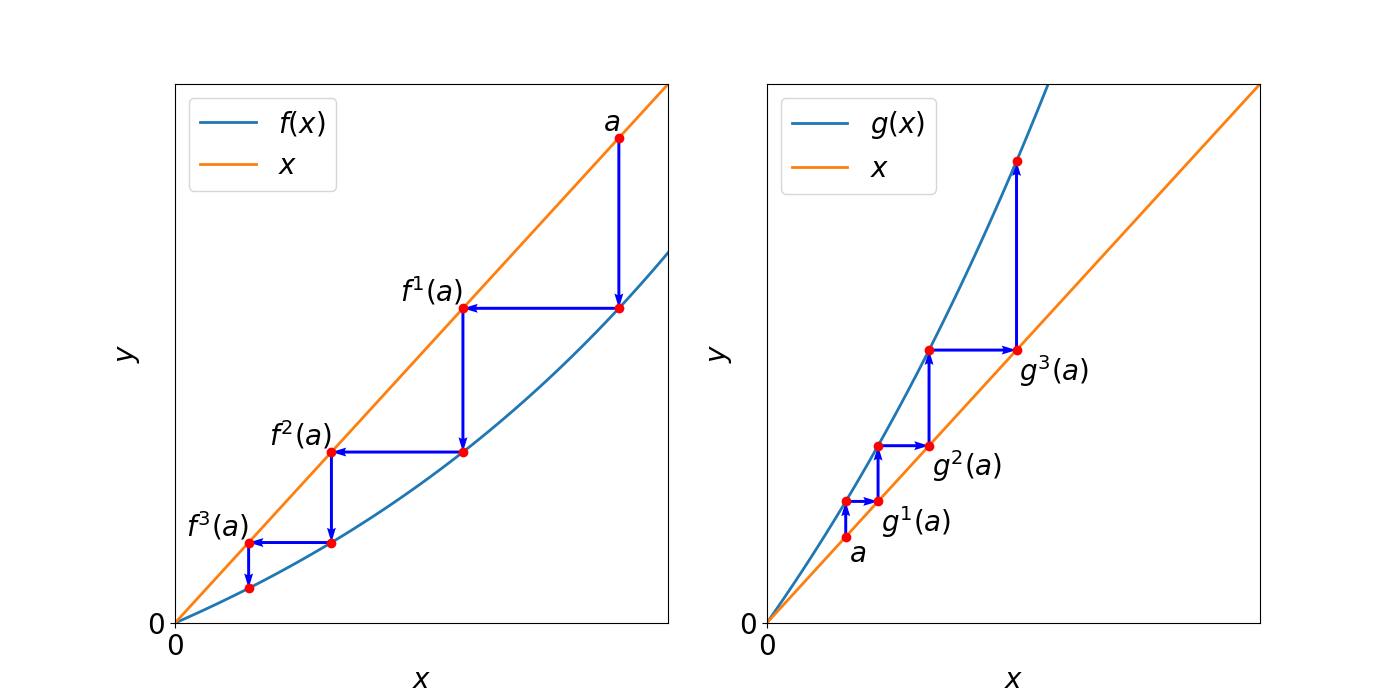
\includegraphics[width=\textwidth]{./figures/stable_and_unstable_fixed_point.png}
	\caption{An illustration of Theorem \ref{th:_stable_unstable_fixed_point}.
	The figure on the left shows function $f(x) = 0.4 e^x - 0.4$, which has a stable fixed point at $x^* = 0$. 
	The figure on the right shows function $f(x) = 1.3 e^x - 1.3$, and its unstable fixed point at $x^* = 0$.}
	\label{fig:stable and unstable fixed point}
\end{figure}

Figure \ref{fig:stable and unstable fixed point} is an illustration of this theorem.
To prove this theorem is a regular exercise using Taylor expansion. 

Assume $x^*$ is a fixed point of the iterated map $f$, whose Taylor expansion is
$$f(x) = f(x^*) + f'(x^*) (x - x^*) + O(x^2).$$

For any $\delta$, evaluate $f(x^* + \delta)$.
Since $x^*$ is a fixed point,
 $f(x^*) = x^*$, and
 $f(x^* + \delta) - f(x^*) = f'(x^*) \delta + O(x^2)$. 
For small enough $\delta$ we can ignore all the terms of degree higher than $2$, and the above equation states $x^*+ \delta$ will eventually converge to $x^*$ if $|f'(x^*)| < 1$, and diverge if $|f'(x^*)| > 1$.

This theorem, though simple, is powerful and is a fundamental part for any rigorous approach of iterated dynamical systems and is also used multiple times in this report (such as in the proof of Observation \ref{th:logistic_bifurcation}). 
As a result, hereby we give another proof using only the classic mean value theorem and $\epsilon-\delta$ definition of limit.

\begin{proof}[Proof of Theorem \ref{th:_stable_unstable_fixed_point}]
	Without loss of any generality we can assume that the stable fixed point is $0$, meaning $f(0) = 0$. 
	If the function $f^*$ has stable point not at $0$ but at $x^*$, we can always investigate the function $f(x) = f^*(x+x^*) - x^*$. 
	
	If for a neighbourhood of $0$, $f' = 0$, we are done, as by mean value theorem $f = 0$ in this neighbourhood, and every $x$ in this neighbourhood converges to $0$ after one iteration.

	If $f' \neq 0$, since $f'$ is continuous, there exists an interval around $0$ such that $f'(x)$ is either strictly positive or strictly negative in this interval (depending on the sign of $f'(x)$), and, since $|f'(0)| < 1$, we can further restrict the interval such that $|f'(x)| < c < 1$. 
	Label this interval as $I$. 
	Notice by construction, this interval is a neighbourhood of $0$, so it must contain $0$.
	
	First, consider $0 < f'(x) < c < 1$ for $x \in I$. 
	For any point $a<0$ and $a\in I$,  $f(a)$ must be small than $0$. 
	Otherwise, the function $f$ will be overall decreasing in the interval $(a, 0)$, and by mean value theorem there will be a point $a^*$ such that $a < a^* < 0$ and $f'(a^*) = \frac{f(a) - f(0)}{a - 0} = \frac{f(a)}{a} < 0$, which is impossible.

	Since $f(a) < 0$, we can further shows that $f(a) > a$. 
	If $f(a) < a$ by mean value theorem there is some point $a^* \in (a, 0)$ such that $f'(a^*) = \frac{f(a) - f(0)}{a - 0} = \frac{f(a)}{a} > 1$, which also impossible.

	As a result the sequence $a, f(a), f^2(a), \cdots$ is monotonically increasing and bounded above by $0$, and by the completeness of the real number it must converge to some number. 
	Assuming it converges to $l < 0$. 
	Let us pick a point $a$ in the interval $(\frac{l}{c}, l)$. 
	That is, $a > \frac{l}{c} \implies \frac{l}{a} > c$ and $f(a) < l$.
	Notice 
	$$
	\frac{f(0) - f(a)}{0 - a} = \frac{f(a)}{a} > \frac{l}{a} > c
	$$
	Where $c$ is the constant defined above such that in the whole interval $|f'(x)| < c$.
	By mean value theorem, there exists a point $b$ in the interval $(a, 0)$ such that $f'(b) = \frac{f(a)}{a} > c$, which is a contradiction.

	All of other cases ($a > 0, f'(0) < 1$) can be proved similarly.
\end{proof}

This theorem does not apply if the derivative of a function at a fixed point is $\pm 1$.
If such is the case the fixed point may be stable or unstable, or it may exhibit more interesting behaviors.
For example, the function $f(x) = e^x - 1$ has a fixed point at $0$.
All $x$ smaller than $0$ will converge to $0$ upon iterations, while all $x$ larger than $0$ will diverge to infinity.

\section{Devaney's Definition of Chaos}

We have used the term chaotic serveral times in this report without rigorous definition. 
In this session we will settle this problem.

One intuition is that every point in the chaotic system can be ``mixed'' with any other point after some time interval. 
This is captured by topological transitivity.
\begin{defn}[Topologically Transitive]
	Let $J$ be a set with a topology.
	The function $f: J \rightarrow J$ is topologically transitive if, for all non-empty open sets $U_1, U_2 \in J$, there exist $k \in \bb{N}$ such that $f^k(U_1) \cap U_2 \neq \varnothing$. 
	Here $f^k$ denotes the composition $\underbrace{f \circ f \cdots \circ f}_{k \text{ times}}$
\end{defn}

The second intuition for chaos is that a small change in the initial condition can lead to a large change in the final condition. 
Lyapunov exponent is a quantitative measure of this, but here we present another analytical definition, which is sensitive dependence on initial condition. This term is coined by Ruelle \cite{Ruelle-1978}.
\begin{defn}[Sensitive Dependence on Initial Conditions]
	Let $J$ be a metric space with the metric $d: J \times J \rightarrow \bb{R}$. The function
	$f: J \rightarrow J$ has a sensitive dependence on initial conditions if there exists some $\delta > 0$ such that for all $x \in J$ and any neighbourhood $X$ containing $x$, there exists $y \in X$ and $n \in \bb{N}$ such that $d(f^n(x), f^n(y)) > \delta$.
\end{defn}

Maybe the most striking fact about chaotic systems is that, although seemingly chaotic, some order still remains.
Since chaos tends to mix all points together, it is natural that some points will return to their original position after certain iterations.
Although we may simply decree that periodic points are infinite, using topology we can state a stronger and more precise definition, that is, the periodic points are dense.

Of course, a point $x$ is a period of period $k$ if $f^k(x)=x$, and dense here is in sense of topology.

Therefore, we have arrived at the following definition.

\begin{defn}[Chaos, Devaney's Definition]\label{def:Devaney_definition_for_chaos}
	Let $V$ be a metric space.
	A function $f: V \rightarrow V$ is chaotic if
	\begin{enumerate}
		\item the set of periodic points are dense in $V$, and
		\item $f$ is topologically transitive,
		\item $f$ has sensitive dependence on initial condition. 
	\end{enumerate}
	
\end{defn}


The definition here is attributed to Devaney \cite{Devaney_green_book_chaos_definition}. 
The first two requirements are purely topological, while the last one requires a metric. 
While in most circumstances topological properties are more generalised than the metric properties, here, surprisingly, as long as $V$ is a metric space (which is part of the assumption), the first two implies the third\cite{Banks}. 
As a result, we only need to check the first two conditions to determine if a function is chaotic.

\begin{thm}[Criterion For Chaotic Function]
	Let $V$ be a metric space. 
	Function $f: V \rightarrow V$ is chaotic as defined in \ref{def:Devaney_definition_for_chaos}
	if and only if its the periodic points are dense $V$ and it is topologically transitive,
\end{thm}

% TODO: Say more about doubling map. 
% TODO: graph, say more in introduction, etc?
% The doubling map is topologically transitive to the map in $S^1$

\begin{example}\label{ex_doubling_map}
	Recall the doubling map $f: [0,1) \rightarrow [0,1)$
	\begin{equation}\label{eq:doubling_map}
	f(x) = 
		\begin{cases}
			2x &\text{ if } 2x < 1 \\
			2x -1 &\text{ if } 2x > 1
		\end{cases}
	\end{equation}
	% TODO: more explanation
	This map can also be regarded as doubling the angles on the unit cycle: $g: S^1 \rightarrow S^1$ given by $ g(\theta) = 2 \theta$.
	
	The doubling map is \textit{chaotic}.

	All non-zero rational points $\frac{p}{q} \in [0,1)$ with odd denominator are periodic points for $f$. 
	The set of these points are dense.
	To show the periodicity, note the images of $\frac{p}{q}$ under repetitive applications of $f$ are $\frac{p}{q}, \frac{2p}{q}, \cdots, \frac{2^k p}{q}, \cdots$.
	We can regard all the numerators as the equivalence classes modulo $q$.
	Since this sequence is infinite and there are only finitely many possibilities for the numerators, some of the numerators must coincide. Let them be $2^k p$ and $2^{k'} p$. 
	Without loss of generality, let $k > k'$, and
	$$
	2^k p \equiv 2^{k'} p \mod q \implies 
	2^{k-k'} p \equiv p \mod q \text{ (as $q$ is odd)},
	$$
	which means $f^{k-k'}(\frac{p}{q}) = \frac{p}{q}$, i.e., $\frac{p}{q}$ is a point of period $k - k'$.

	To show $f$ is topologically transitive is even easier. 
	For any non-empty open set $U \in [0,1)$, by definition there exists an open interval $J = (x, x+ \delta) \subseteq U$. 
	$J$ has diameter $\delta$, $f(J)$ has diameter $2 \delta$, and $f^k(J)$, $2^k \delta$. 
	Since the length of $[0,1)$ is $1$, after some finite iteration $f^k(J)$ would covers all of $[0,1)$ and intersect any other open sets.

	By generalising this proof it is clear any maps in the form 
	$$
	g: S^1 \rightarrow S^1; g(\theta) = r \theta, r \in R
	$$
	are chaotic.
\end{example}

\section{Topological Conjugacy}

To prove the doubling map is chaotic is a gentle exercise. 
To directly find the points of periodicity and prove that a general function is topologically transitive is difficult.
Instead, we can circumvent these challenges by exploiting topological conjugacy.

\begin{defn}[Topological Conjugacy]
Funcitons $f: X \rightarrow X$, $g:  Y \rightarrow Y$ are topologically conjugate if there exist a homeomorphism $\phi: X \rightarrow Y$ such that 
$\phi \circ f = g \circ \phi$,
i.e, the following diagram commutes.
\begin{center}
    \begin{tikzcd}
        X \arrow[r, "f"] \arrow[d, "\phi" swap] & X \arrow[d, "\phi"] \\
        Y \arrow[r, "g"] & Y
    \end{tikzcd}
\end{center}

The maps $f,g$ are semiconjugate if there exists a continuous surjection, $\psi$ such that $\psi \circ f = g \circ \psi$.
\end{defn}


To rephrase the definition, $f $ and $g$ are conjugate if there exists a homeomorphism $\phi$ such that $f = \phi^{-1} \circ g \circ \phi$.
So $f^{n} = \phi^{-1} \circ g^{n} \circ \phi$; that is $f^n$ is conjugate to $g^n$.

Topological conjugacy is an equivalence condition. 
Function $f$ is conjugate to itself by the identity map. 
$\phi \circ f = g \circ \phi$ implies $f \circ \phi^{-1} = \phi^{-1} \circ g$, so $g$ is also conjugate to $f$.
At last we need to prove transitivity, which is illustrated in the following scheme.
\begin{center}
    \begin{tikzcd}
        X \arrow[r, "f"] \arrow[d, "\phi" swap] & X \arrow[d, "\phi"] \\
        Y \arrow[r, "g"] \arrow[d, "\phi'" swap] & Y \arrow[d, "\phi'"] \\
        Z \arrow[r, "h"] & Z \\
    \end{tikzcd}
\end{center}
If $f$  is conjugate to $g$ via $\phi$, and $g$ is conjugate to $h$ via $\phi'$, $\phi' \circ \phi \circ f = \phi' g \circ \phi = h \circ \phi'' $, which means $f$ is conjugate to $h$ via $h' \circ h$. 



Topological semiconjugacy only requires a continuous surjection, $\psi$, such that $\psi \circ f = g \circ \psi$. 
As $\psi$ may not have an inverse, semiconjugacy can not be an equivalence condition.
Nevertheless, if $f$ is semiconjugate to $g$, so is $f^{k}$ to $g^{k}$ for any $k \in \bb{N}$. 
This is because 
$$
	\psi \circ f ^k = \psi \circ f\circ \cdots \circ f = g \circ \psi \circ f \cdots \circ f = \cdots = g^k \circ \psi
$$

 % TODO: verify this is true
If $f$ is conjugate to $g$, necessarily $f$ is semiconjugate to $g$ and $g$ is semiconjugate to $f$. 
However, if $f$ is semiconjugate to $g$ and $g$ is semiconjugate to $f$, $f$ is not necessarily conjugate to $g$. 

Chaotic behaviours are \emph{preserved} by conjugacy.


\begin{thm}[Semiconjugacy preserves Chaos]\label{th_semicong_chaos}
	If $f$ is semiconjugate to $g$ and $f$ is chaotic, $g$ also is.
\end{thm}
% TODO: can g chaotic implies f also is if f is semiconjugate to g?
% FIND counter example

\begin{proof}
	Let $f: X \rightarrow X$, $g:  Y \rightarrow Y$, and let $\psi$ be the promised continuous surjection $X \rightarrow Y$ such that
	$\psi \circ f = g \circ \psi$. 
	Since $\psi$ is conituously surjective, for any non-empty open set $M \in Y$, $\psi^{-1}(M)$ is an non-empty open set in $X$.

	Let us first prove that the set of periodic points of $g$ is dense.
	For any $x$ such that $f^k(x) = x$, notice that $g^k \circ \psi (x) = \psi \circ f^k (x) = \psi(x)$. 
	This means, if the set of periodic points of $f$ is $X$, $\psi(X)$ is a subset of the set of periodic point of $g$.

	For the sake of contradiction assuming $\psi(X)$ is not dense in $Y$. 
	This means there is a open set $M \subset Y$ such that $M \cup \psi(X) = \emptyset$.
	The preimage $\psi^{-1}(M)$ is an non-empty open set of $X$, and by assumption, it does not contains any periodic points of $f$, which is a contradiction.

	To prove that $g$ is topologically transitive, consider any non-empty open set $M, N \in Y$, and $\psi^{-1}(M), \psi^{-1}(N)$ are non-empty open set in $X$. 
	By assumption there exists some $k$ such that $f^k(\psi^{-1}(M)) \cap f^k(\psi^{-1}(N)) \neq \emptyset$, this means 
	\begin{align*}
		g^k(M) \cap g^k(N) 
		&= \underbrace{\psi \circ f^k(\psi^{-1}(M))}_{\text{by topological semiconjugacy}} \cap \psi \circ f^k(\psi^{-1}(N)) \\
	    &\subset \psi( f^k(\psi^{-1}(M)) \cap  f^k(\psi^{-1}(N))) \neq \emptyset
	\end{align*}
\end{proof}

Since conjugacy impies semiconjugacy on both directions, we have the following important proposition.

\begin{prop}[Conjugacy Class share chaotic behavior]\label{prop_conj_chaos}
	If $f$ is conjugate to $g$, $f$ is chaotic if and only if $g$ is chaotic.
\end{prop}

There are abundant examples of topological conjugacy.

\begin{example}
	In an open interval $[-\epsilon_1, \epsilon_2] \in \bb{R}$,
	$f: [-\epsilon_1, \epsilon_2] \rightarrow [-\epsilon_1, \epsilon_2]$
	is conjugate to 
	$g: [-\epsilon_1 + a, \epsilon_2 + a] \rightarrow  [-\epsilon_1 + a, \epsilon_2 + a]$
	where $g(x)= f(x -a) + a$ via $\phi(x) = x + a$.

	For a concrete example, consider the map 
	$f: [0,1] \rightarrow [0,1]$
	defined as $f(x) = 4x(1-x)$,
	which is conjugate to 
	$g(x): [-\frac{1}{2}, \frac{1}{2}] \rightarrow [-\frac{1}{2}, \frac{1}{2}]$
	defined as $g(x) = -4x^2 + \frac{1}{2}$ 
	through $\phi(x) = x -\frac{1}{2}$, i.e., $ \phi \circ f=  g \circ \phi$.
\end{example}

\begin{example}
	For closed interval $[-\epsilon_1, \epsilon_2] \in \bb{R}$. 
	$f: [-\epsilon_1, \epsilon_2] \rightarrow [-\epsilon_1, \epsilon_2]$
	is conjugate to 
	$g: [-\frac{\epsilon_1}{a}, \frac{\epsilon_2}{a}] \rightarrow [-\frac{\epsilon_1}{a}, \frac{\epsilon_2}{a}]$
	where $g(x)= \frac{1}{a}(ax)$ via $\phi(x) = ax$.


	As another concrete example, the map $f: [0,1] \rightarrow [0,1]$
	defined as $f(x) = -4x^2 + \frac{1}{2})$,
	is conjugate to 
	$g(x): [-1, 1] \rightarrow [-1, 1]$
	defined as $g(x) = 2x^2 - 1$
	through $\phi(x) = -2x$.
\end{example}

\begin{example}
	Consider the doubling map $f: [0,\pi) \rightarrow [0, \pi)$ defined thus: 
	$$
	f(\theta) = 
		\begin{cases}
			2 \theta &\text{ if } 2x <  \pi \\
			2 \theta - \pi &\text{ if } 2x > \pi
		\end{cases}
	$$
	
	This map is doubling the angle of the unit circle.

	$f$ is semiconjugate to $g: [-1, 1] \rightarrow [-1, 1]$ defined as $g(x) = 2x^2 - 1$ through $\cos(x)$.

	Example \ref{ex_doubling_map} shows that the doubling map is chaotic, so is $g$.
\end{example}

\begin{example}\label{ex_logistic_and_doubling}
	The above 3 examples shows that the doubling map is semiconjugate to the logistic map $L_1(x) = 4x(1-x)$.
\end{example}

\begin{example}\label{ex:logistic and tent}
	The logistic map $L_1(x) = 4x(1-x)$ in the interval $[0,1]$ is topologically conjugate to the tent map defined as 
	\begin{equation}
		f(x) = 
		\begin{cases}
			2x   &\text{ if } 0<x \leq \frac{1}{2} \\ 
			2-2x &\text{ if } \frac{1}{2} < x \leq 1
		\end{cases}
	\end{equation}
	via the map $h: [0,1] \rightarrow [0,1]$ defined as $h(x) = \sin^2(\frac{\pi x}{2})$.
	This can be verified by the simple computation $L_1 \circ h = h \circ f$.

	Since $L_1$ is chaotic, so is the tent map.
\end{example}

\chapter{Bifurcations in Discrete Dynamical Systems}\label{chapter:bifurcation}
The logistic map, due to its ever-repeating presence in this report, will now be formally introduced. It has become one of the staple examples of chaotic systems due to its simple form yet countless fascinating and complex properties. Furthermore, it will be the key to deriving Feigenbaum's universal constants in the final section.

\section{The Logistic Map as a Model for Population Growth}

One-dimensional recursive equations $x_{n+1} = f(x_n)$ are used for modelling various dynamical systems. 
Notwithstanding their simplicity, many of these maps exhibit extremely complicated properties which are also present in their more complicated counterparts.

Consider, for example, bacteria population in discrete time intervals. 
If the population is low and resource abundant, the rate of growth is in proportion to the population, which gives rise to the following equation
\begin{equation}\label{eq:1d iterative map}
p_{t+1} = p_{t} b,
\end{equation}
where $p_{t}$ is the population of the bacteria at the discrete time $t$ and $b$, as a constant, is the static birth rate for bacteria whose value will depend on the model.

The limited resource will slow down the rate of growth of the bacteria as the population increases, and the relation will become 
\begin{equation}\label{eq:p times beff}
	p_{t+1} =  p_{t} \be
\end{equation}

The usual assumption is that $\be$ is close to $b$ when the population is low, and there is a threshold above which the population will decrease. 
At the threshold $\be$ will be zero.

The simplest equation for modelling $\be$ is the linear equation
\begin{equation} \label{eq:b_effective}
\be = b - ap,
\end{equation}
where $a$ is another constant depending on the model.
Combining the equations \eqref{eq:p times beff} and \eqref{eq:b_effective}, the recursive formula becomes 
$$
p_{t+1}  = b p_t - ap_t^2
$$

Substituting $p_{t} := \frac{b}{a} x_{t}, \lambda := \frac{b}{4}$, we obtain
$$
x_{t+1} = 4 \lambda x_t(1-x_t) 
$$
Thence comes the standard forms of the logistic map depending on one variable $\lambda$
\footnote{
Some sources defined the logistic map as $L^*_{\lambda}(x) = \lambda x(1-x)$ without the constant 4. 
In this report, however, we will use equation \ref{eq_logistic}, which has the advantage that the maximum value attained by $\L(x)$ at $\frac{1}{2}$ is $\lambda$, and it will also be consistent to the definitions of other class of functions discussed later in the report.
}
\begin{equation}\label{eq_logistic}
	L_{\lambda}(x) = 4 \lambda x(1-x)
\end{equation}

% graph produced by `logistic_map_diff_lambda`
\begin{figure}[t]
	\centering
	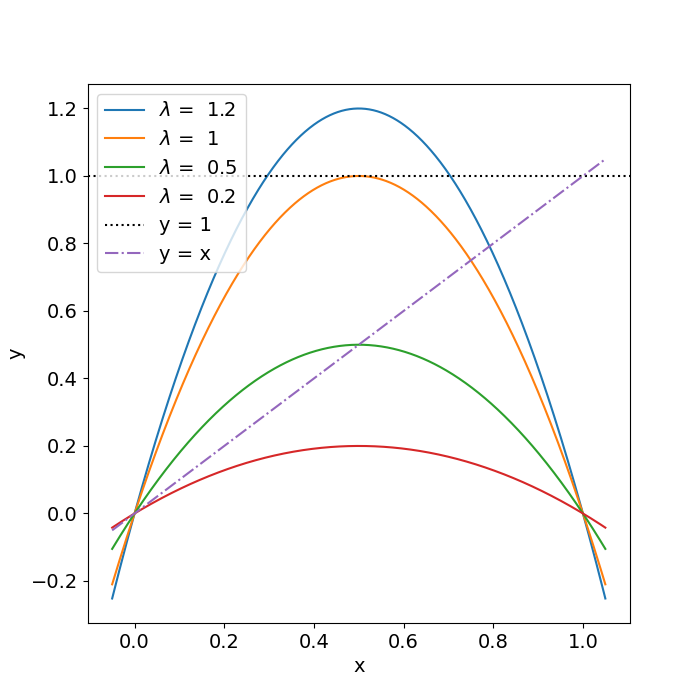
\includegraphics[width=0.7\textwidth]{./figures/logistic_map_diff_lambda.png}
	\caption{Graphs of logistic map $L_{\lambda}(x) = 4 \lambda x(1-x)$ for different $\lambda$ compared with the line $y=x$ and $y = 1$.} 
	\label{fig:logistic_map_diff_lambda}
\end{figure}

% The dynamical system in discrete time interval generated by the iterations of the logistic map is the study of this session.

Scrutinising the class of discrete logistic functions plotted in figure \ref{fig:logistic_map_diff_lambda}, some of their properties are obvious:

\begin{enumerate}
	\item $\L(x)$ is a smooth function;
	\item $\L(x)$ concaves downwards, that is, $\L(x)'' < 0$;
	\item $\L(x)$ attains a unique maximum at $x = \frac{1}{2}$, and $L_{\lambda}(\frac{1}{2}) = \lambda$; and,
	\item when $0 \leq \lambda$ and $x$ is restricted to the domain $[0, 1]$, $\L(x)$ is a two-to-one non-surjective (except for $\lambda = 1$) function $\L(x): [0,1] \rightarrow [0,\lambda]$. 
\end{enumerate}


We can check if this model would work as expected by comparing it to its continuous counterpart 
\begin{equation}\label{eq_logistic_continuous}
	\frac{dp}{dx} = c p(x) (1-p(x)),
\end{equation}

where $c$ is some arbitrary constant denoting the rate of growth. 
The unique solution to this ordinary differential equation with the initial condition $p(0) = \frac{1}{2}$ is 
$$
p(x) = \frac{e^{cx}}{1+e^{cx}}.
$$
\begin{figure}
	\centering
	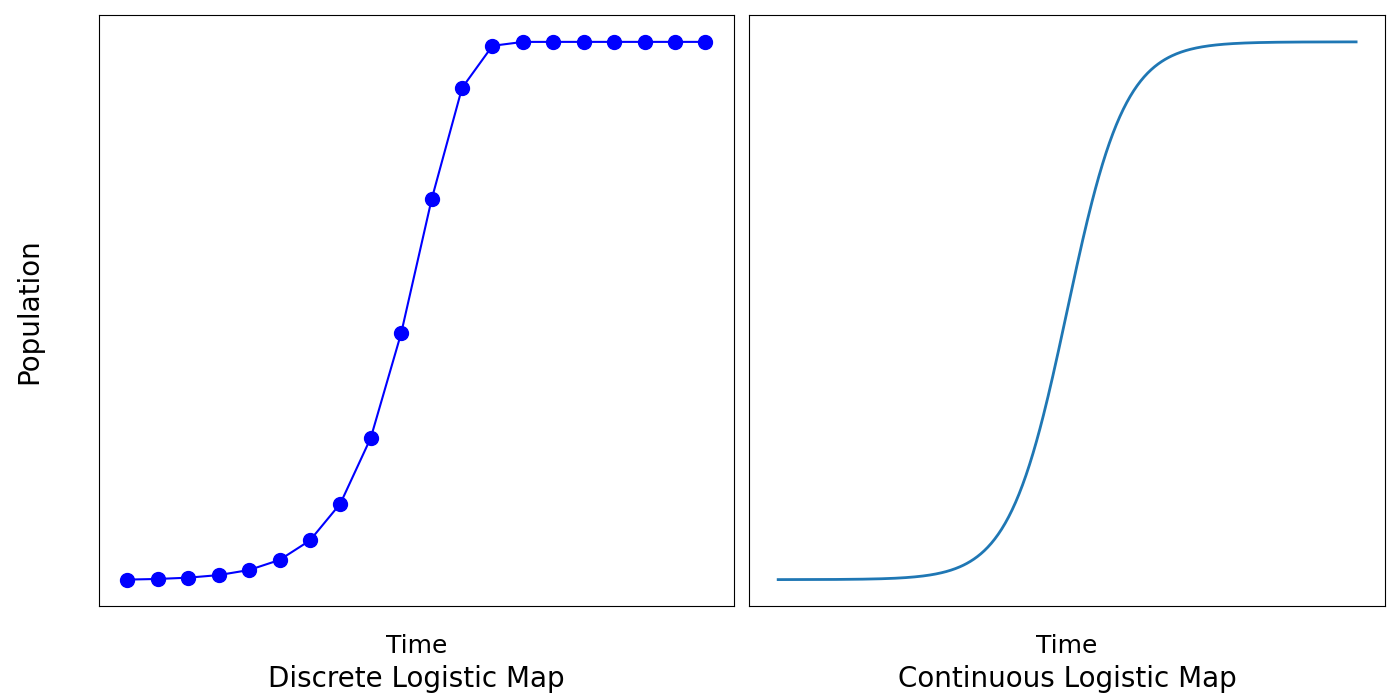
\includegraphics[width=0.8\textwidth]{./figures/con_vs_discrete_logistic_map.png}
	\caption{The population of the bacteria modelled by the discrete (left) v.s. continuous (right) logistic map. 
	The discrete case is modelled by $\lambda = 0.5$ and $x_0 = 0.0003$, and the continuous case has $c=1$.}
	\label{fig:con_vs_discrete}
\end{figure}
The graph of the populations modelled by \eqref{eq_logistic} and \eqref{eq_logistic_continuous} are shown in Figure \ref{fig:con_vs_discrete}.
Indeed, at least for the selected value of $\lambda$ and $c$, the population modelled by the two maps are similar.

Having settled that the discrete logistic map is a good simplification for the already-simplified equation \eqref{eq_logistic_continuous} as a model for population growth, you may wonder why we bother studying such a simple equation. 
The reason is, as simple as it seems, that the iteration of equation \eqref{eq_logistic} gives rise to some extremely complicated dynamical systems with many surprising properties. 
These interesting dynamics are also observed in the continuous case and is the study of the next session.

It shall be stressed, at the end of this session before we go in depth into the theoretical discussions, that no impression shall be made to assume that one-dimensional discrete iterative maps are only useful as a crude model for bacteria population growth. 
There are abundant examples where equation \eqref{eq:1d iterative map} can be used as a model, some up to a strikingly high accuracy. 
For example: in genetics, it is used when investigating on the frequency of the genotype \cite{genotype}; in economics, modelling the relationship between commodity quantity and price \cite{economics}; and in social science, on the propagation of rumours \cite{social_science}, among many others.


\section{Logistic Bifurcations}

To make our terminology precise and avoid any possible confusion, we shall reiterate that the focus of this session is the one-dimensional discrete dynamical system depending on one parameter $\lambda$, generated by the iterations of the logistic map. 
Explicitly, it is the sequence $x_0, x_1, \dots$, where $x_0$ is the initial condition, and $x_{n+1} = \L(x_n)$, as defined in \eqref{eq_logistic}.

The first step of studying this system is to plot it with different initial values $x$ and parameters $\lambda$. Only $0 \leq \lambda \leq 1$ and $0 \leq x_0 \leq 1$ are considered, so that $\L(x)$ is a map from $[0,1]$ to $[0,1]$. 

% graph produced by `modelling_pop_with_diff_logistic_maps` in `graph_qc` repo
\begin{figure}[htbp]
	\centering
	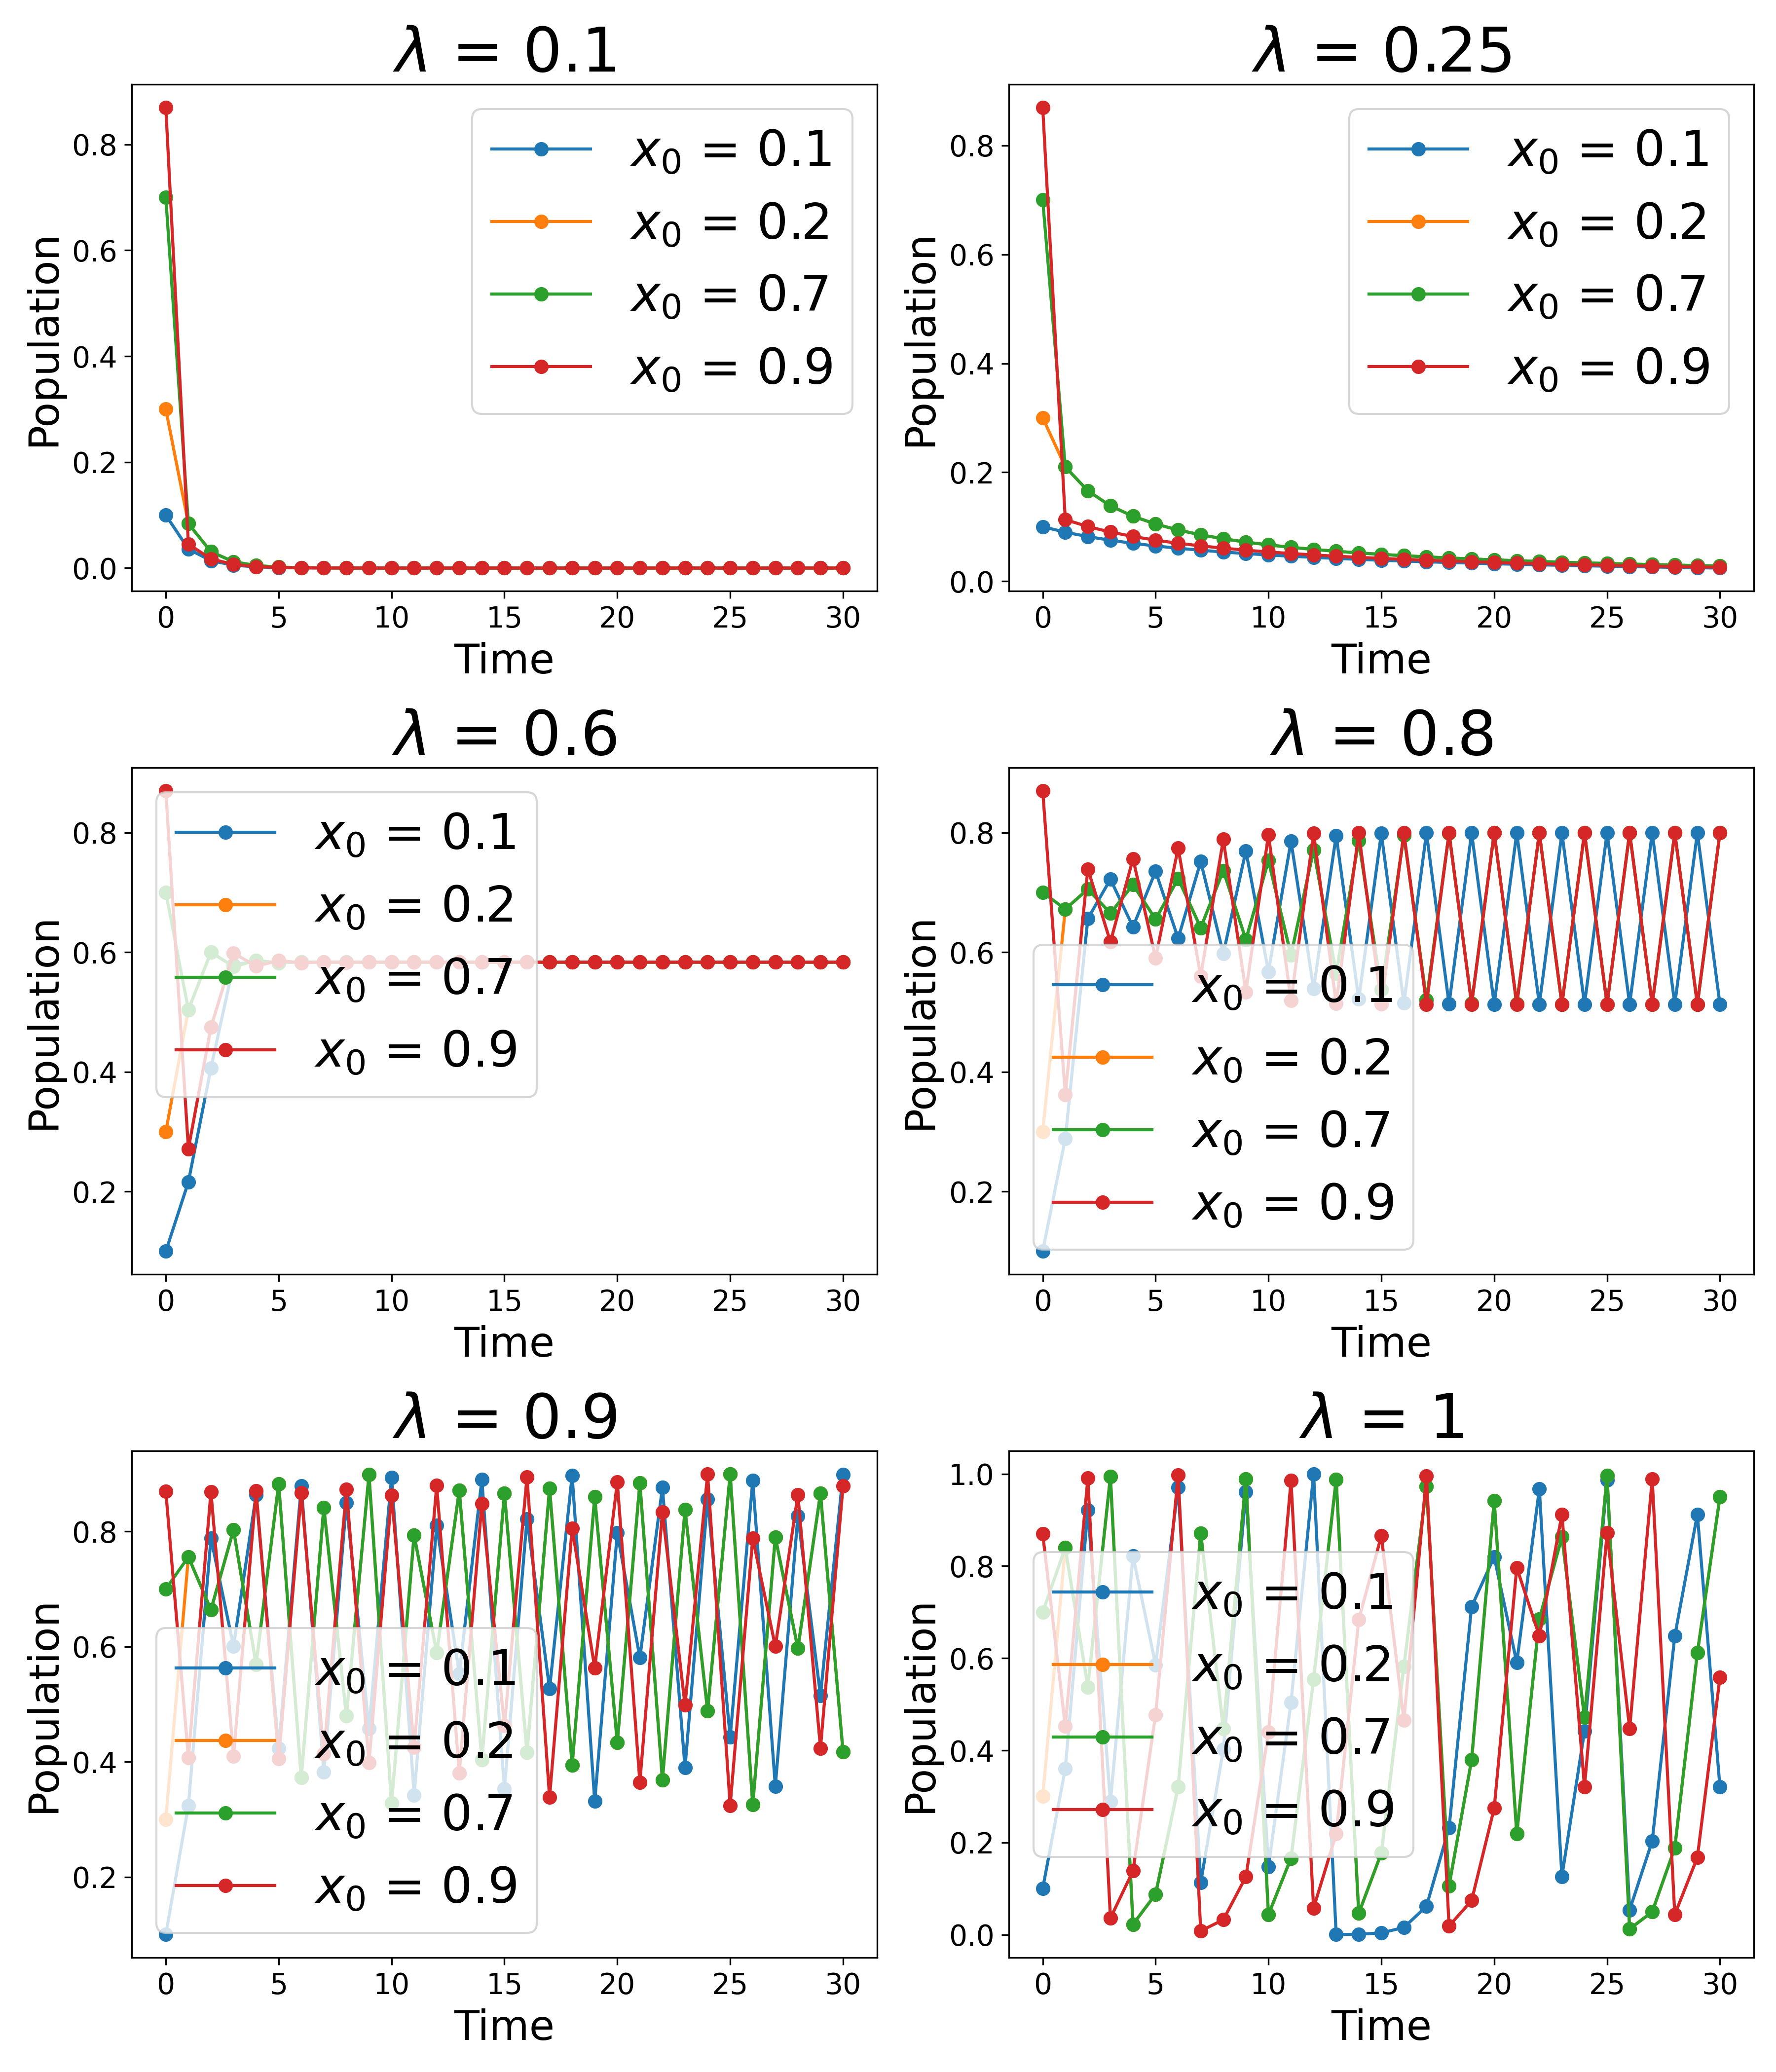
\includegraphics[width=0.9\textwidth]{./figures/various_iterating_logistic_map.png}
	\caption{Iterating the logistic map with different initial values and $\lambda$. All graphs are produced by setting a $x_0$ and $\lambda$, and iterating $x_{n+1} = L_{\lambda}(x_n)$, and plotting all $x_n$ values respect to iteration number $n$.}
	\label{fig:various_iter_logistic}
\end{figure}

There are several immediate observations upon looking at Figure \ref{fig:various_iter_logistic}.
When $\lambda = 0.1$ and $0.25$, it seems $\lim_{n \rightarrow \infty} x_n = 0$, regardless of the value of $x_0$.
For $\lambda = 0.6$, $\lim_{n \rightarrow \infty} x_n = l \neq 0$. 
(We can show that $l = \frac{7}{12}$ by Theorem \ref{th:_stable_unstable_fixed_point}.)

When $\lambda = 0.8$, $x_n$ no longer converges but oscillates in a stable two orbit. 
For $\lambda = 0.9$ and $\lambda = 1$, it is not clear if $x_n$ has any stable orbits or sensible patterns, and the best epithet for them would be `chaotic'.

For all cases, it seems like any initial condition, $x_0$, upon iteration, will eventually tend to some common dynamical behaviour depending only on $\lambda$.
The scatter plot in Figure \ref{fig:logistic bifurcation overview} is produced to capture the behaviour of $x_n$ as $n \rightarrow \infty$ for various intervals of $\lambda$.
These graphs are produced by picking a $\lambda$ and a random $x_0 \in [0,1]$, producing $x_{1} = \L(x_0), x_{2} = \L(x_1), \dots$ through thousands of iterations, ignoring the first several hundred $x_i$s, and plotting the rest of the $x_i$ on the coordinate $(x_i, \lambda)$. 
By repeating this process for one thousand equally spaced $\lambda \in [0,1]$, the bifurcation diagram is obtained.

These pictures of bifurcation are indeed spectacular. 
For $\lambda$ between $0$ and $a_0 = 0.25$, there is a stable fixed point $x = 0$.
When $\lambda$ becomes greater than $a_1 = 0.25$, $0$ is no longer the stable fixed point, but there is another unique stable fixed point greater than $0$.
Precisely when this stable fixed point becomes unstable, around $\lambda = a_2 \approx 0.77$, a stable two-cycle appears.
The stable two-cycle, again, disappears around $\lambda = a_3 \approx 0.86$, at which point a stable 4-cycle appears. 
This process of periodic doubling of the stable orbit, which seems to continue indefinitely, is denominated as \emph{periodic doubling bifurcation}.\footnote{
	The word bifurcation comes from medieval Latin bifurcātus, literally meaning two-forked. Here, it is used figuratively to describe the process of a single stable orbit forking into two.
	
	Bifurcations, in general, mean the change of the behaviour of dynamical systems as parameters vary.
	For systems depending only on one parameter, there are only three kinds of generic bifurcation: periodic doubling, tangent, and inverse periodic doubling \cite{Chaos_in_DS}.
	In this report, we will only touch on periodic doubling bifurcation.
	Bifurcation, in general, has very rich theory and is applicable to a large class of dynamical systems, including continuous ones and those of higher dimensions. \cite{dynamical_systems_v}.
}

Upon closer inspection of the sub-figures of Figure \ref{fig:logistic bifurcation overview}, zoomed around the windows of bifurcation, each stable orbit and bifurcation pattern seems to be self-similar, and all stable orbits cross the line $y = 0.5$ for some $\lambda$.

Periodic doubling bifurcations, however, do not exhaust the whole spectrum of $[0,1]$, and $a_{n}$, which are the values of $\lambda$ at which bifurcations occur, seem to converge to some limit as $n \rightarrow \infty$. 
This limit is labelled as $a_{\infty}$.
For $\lambda > a_{\infty}$, there are no longer any obvious patterns and the overall behaviour is best described as chaotic. 
Nevertheless, in this chaotic region there are windows for stable orbits of odd periods which are not observed for $\lambda < a_{\infty}$ (the term window describing an interval of $\lambda$ for which a stable orbit exists is introduced by May \cite{May_Nature}).
Examples are $\lambda \approx 0.957$ for a 3-cycle and $\lambda \approx 0.934$ for a 5-cycle.

Before moving to full mathematical mode and start proving, for the last time in this report we shall look back to the real world. 
As will be shown in the next session, periodic doubling bifurcation is not unique to the logistic map, but is a common behaviour for a large class of functions sharing very moderate restrictions. 
Many real world systems, such as population and density of genotype, which can be modelled by one dimensional iterative maps, exhibit dramatic variations in quantity respective to time \cite{colorado_potato_beetle}.
This behaviour has baffled biologists, many of whom have attributed the cause to the inaccuracy of measurements and perturbations from the environment. 
The fact that bifurcation is a universal phenomenon for iterative maps, however, may suggest that these variations may be due to the inherent nature of the system itself \cite{genotype}.


The following paragraph lists some of the key observations of bifurcation and the sketches of their proofs.

\begin{figure}[htbp]
	\centering
	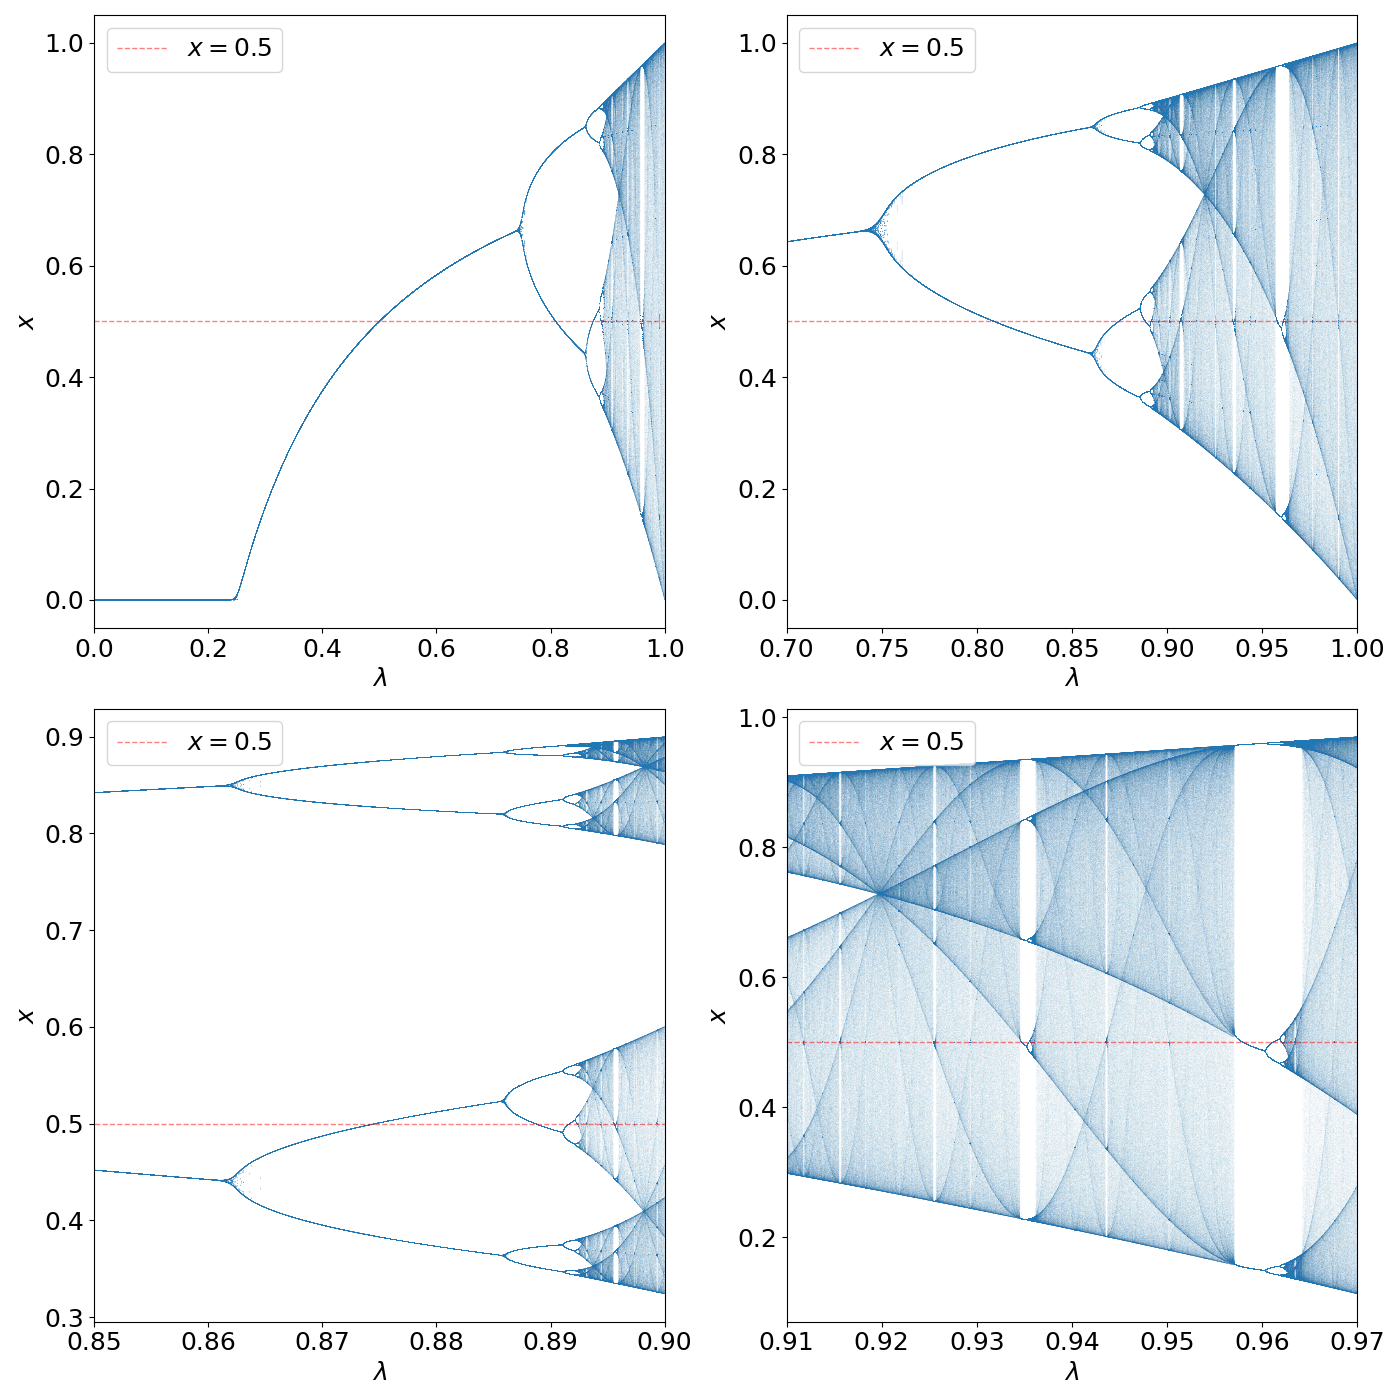
\includegraphics[width=\textwidth]{./figures/logistic.png}
	\caption{
		The graph of logistic bifurcation.
		Each of the subfigures were produced by iterating the logistic map $\L$ with a random starting value $x_0$ to obtain $x_{n+1} = \L(x_n)$ etc., discarding the first several hundred values, and graphing each of the subsequent values as a faint, semi-transparent blue dot at the coordinate $(x, \lambda)$.
		The graph on upper left is the overview of logistic bifurcation on the interval $0 \leq \lambda \leq 1$; upper right and lower right zoomed into the area of periodic doubling, recording $0.7 \leq \lambda \leq 1$ and $0.85 \leq \lambda \leq 0.9$, respectively. Lower right is a zoomed in view of the chaotic region for $ 0.91 \leq \lambda \leq 0.97$. 
	}
	\label{fig:logistic bifurcation overview}
\end{figure}

\begin{observation}[Logistic Bifurcation]\label{th:logistic_bifurcation}
	Let $L_{\lambda} = \lambda 4x(1-x) $ be the logistic function as defined in \eqref{eq_logistic}.
	The dynamical system in a discrete time interval generated by the iteration of the logistic map has the following properties.

	\begin{enumerate}
		\item For $0 < \lambda < a_0 = \frac{1}{4}$, the system has a unique fixed point at $x = 0$. \label{log_fix_0}

		\item For $a_0 <\lambda < a_1 = \frac{3}{4}$, the fixed point at $x=0$ is no longer stable, but a new stable non-zero fixed point emerges. \label{log_fix_1}

		\item When $\lambda$ becomes greater than some value $a_2$, the one cycle becomes unstable, and a stable two cycle appears. 
		Similarly, the 2 cycle will bifurcate into a 4 cycle at $a_3$, $2^n$ cycle to $2^{n+1}$ cycle etc. until $\lambda \rightarrow a_{\infty}$. 
		\label{log_periodic_doubling}
		\item Specifically, for any $\lambda$ there is at most one set of stable orbits. \label{log_at_most_one_stable_orbit}

		\item \label{log_simul_stable_or_unstable}
		Assume for certain $\lambda$ there is an $n$ cycle. That is, there exists distinct $x_1, \cdots, x_n$ such that $\L(x_1) = \L(x_2), \L(x_2) = \L(x_3), \cdots, \L(x_n) = \L(x_1)$.
		Necessarily $x_1, \cdots, x_n$ are $n$ fixed points of $\L^n$. 
		These $n$ distinct fixed point for $\L^n$ must be simultaneously attracting fixed points or repelling fixed points for a given $\lambda$, possibly except for a set of measure zero.

		\item \label{log_cross_half} 
		Let $[a, b]$ be a window of stable orbit of period $n$.
		There exists $\epsilon \in [a, b]$ such that $L_{\epsilon}^n(0.5) = 0.5$. 
		This is the intuitive observation that every orbit must cross the line $x = 0.5$, as shown in the zoomed in view of the bifurcation in figure \ref{fig:logistic bifurcation overview}.

		\item \label{log_closest_branch}
		Observing Figure \ref{fig:logistic bifurcation overview} of the bifurcation pattern in a windows of $2^n$ stable orbits. 
		The previous observation states that there exists a certain $\lambda$ such that $0.5$ is part of the stable orbit, that is $L_{\lambda}^{2^n}(0.5) = 0.5$.
		There is another orbit closest to $0.5$, which spawned from the same bifurcation point.
		The value of this point is $\L^{2^{n-1}}(0.5)$.


		\item  \label{log_chaos_at_1}
			When $\lambda = 1$, the map exhibits chaotic behaviour, defined in Definition \ref{def:Devaney_definition_for_chaos}. 
	\end{enumerate}
\end{observation}

\begin{figure}[htbp]
	\centering
	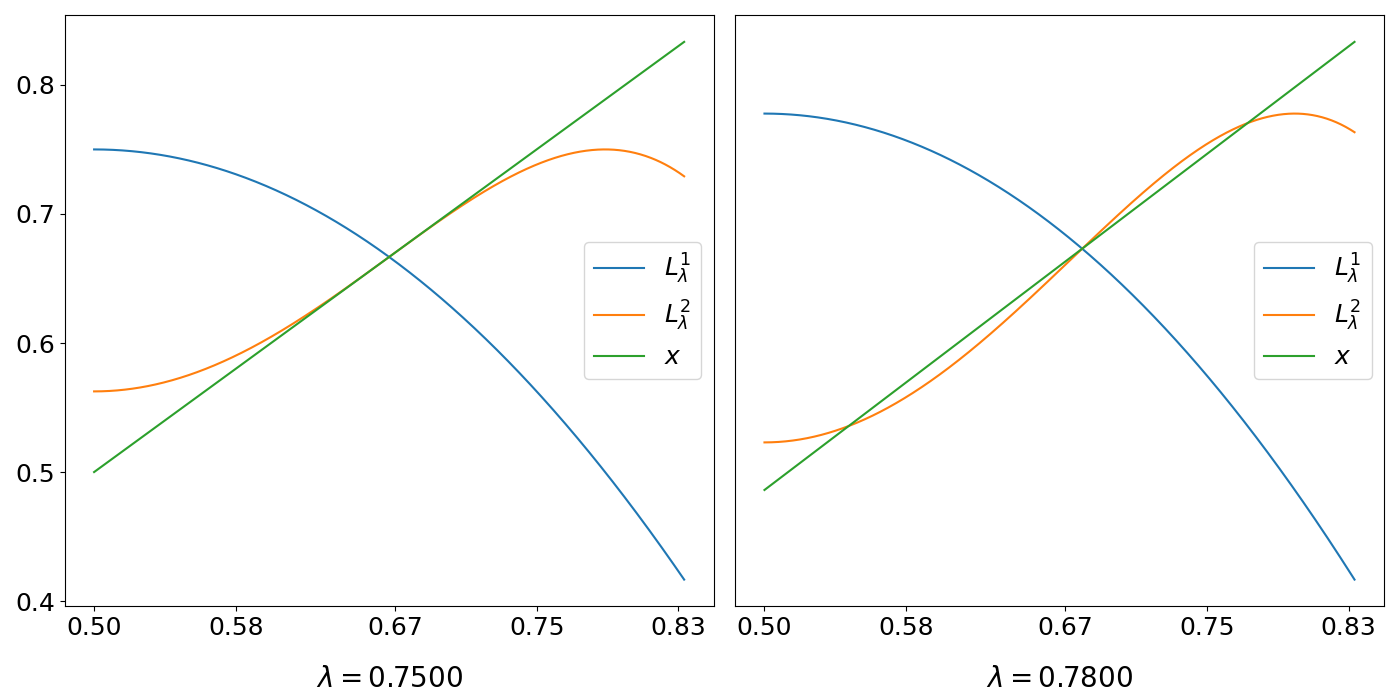
\includegraphics[width=0.8\textwidth]{./figures/logistic_map_around_bifurcation.png}
	\caption{
		$\L, \L^2$ and the function $y=x$ are graphed and zoomed in around the fixed point for $\lambda = 0.75$ and $\lambda = 0.78$, where the bifurcation takes place.
		For $\lambda < 0.75$, as can be seen from Figure \ref{fig:logistic_map_diff_lambda}, the system as a unique stable point. This point loses its stability and a stable two-cycle appears just after $\lambda$ increases above $0.75$.
		This is because, as shown on the right, precisely when the stable fixed point became unstable, the graph of $\L^2$ will have two more intersection with the line $y=x$, which becomes the stable two orbit.
	}
	\label{fig:point_of_bifurcation1}
\end{figure}

\begin{figure}[htbp]
	\centering
	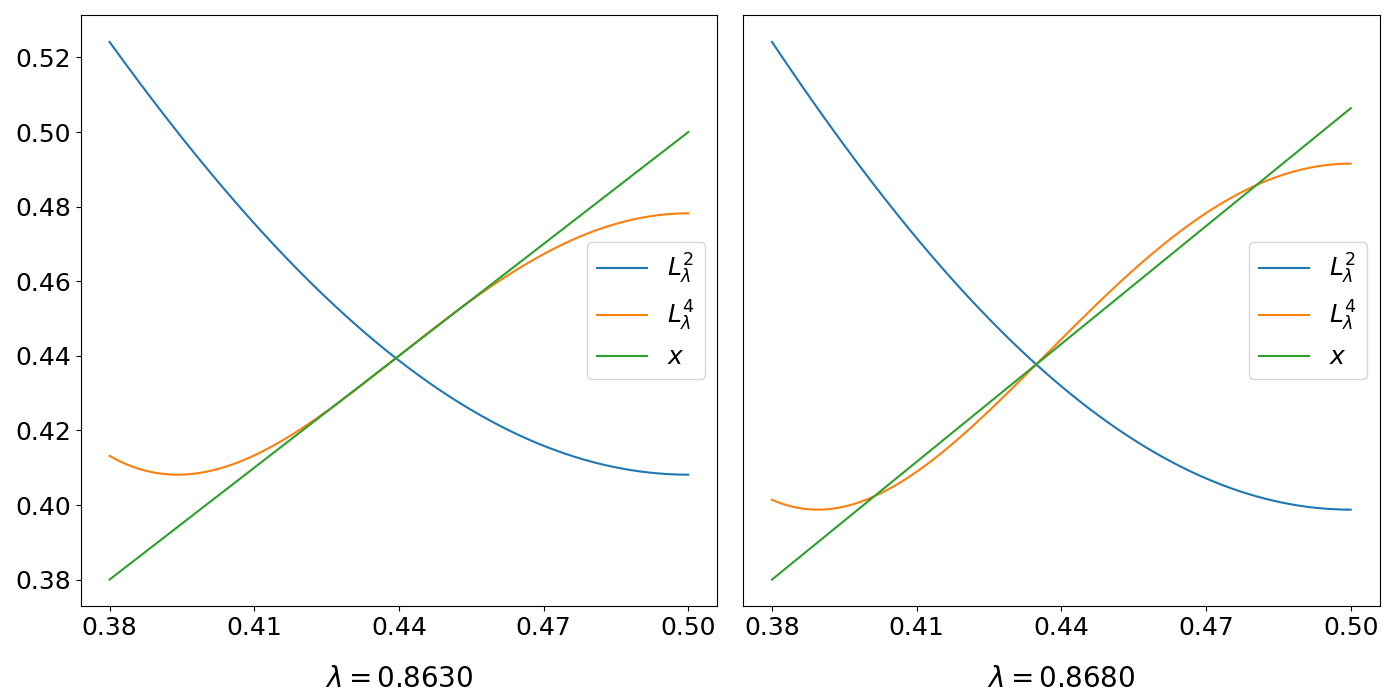
\includegraphics[width=0.8\textwidth]{./figures/logistic_map_around_bifurcation_2.png}
	\caption{Showing $\L^2, \L^4$ and $y=x$ close to one point of second bifurcation similar to Figure \ref{fig:point_of_bifurcation1}}.
	\label{fig:point_of_bifurcation2}
\end{figure}

\begin{proof}[Proof of \ref{th:logistic_bifurcation}.\ref{log_fix_0} and \ref{th:logistic_bifurcation}.\ref{log_fix_1}]
	The fixed point for $\L(x)$ is exactly the solution of the equation $\L(x) = x$, which are $x_0 = 0$ and $x_1 = 1 - \frac{1}{4\lambda}$. 
	$|L_{\lambda}(x_0) | = 4 \lambda < 1$ for $0 < \lambda < \frac{1}{4}$, so by Theorem \ref{th:_stable_unstable_fixed_point}, $x_0$ is a stable fixed point in this interval.
	The argument for $x_1$ is similar.
\end{proof}

% TODO: This prove needs improvements
\begin{proof}[Demonstration of \ref{th:logistic_bifurcation}.\ref{log_periodic_doubling}]
	The proof of this phenomenon again exploits Theorem \ref{th:_stable_unstable_fixed_point}.

	Let us concentrate on $\lambda^*$ at which the fixed point $a$ becomes unstable; that is, $L_{\lambda*}' a  = - 1$ and for any $\lambda > \lambda^*$, the derivative at the fixed point is smaller than $-1$, thus $a$ becomes an unstable fixed point. (This observation is made obvious in Figure \ref{fig:point_of_bifurcation1}.)
	Necessarily, $\frac{d}{dx}L_{\lambda^*}^2 a = L'_{\lambda^*}(a) \cdot L'_{\lambda^*}(a) = 1$,
	and for any $\lambda > \lambda^*$, $\frac{d}{dx}L_{\lambda}^2a'> 1$, where $a'$ is the new fixed point.

	Since $\frac{d}{dx}L_{\lambda}^2(a') > 1$, by mean value theorem for some $\delta > 0$, $\L^2(a' - \delta) < a' - \delta$, and $\L^2(a' + \delta) > a' + \delta$. 
	Observe that $\L^2(1) = 0 < 1$, so by intermediate value theorem there must be some point $b > a' + \delta$ such that $\L^2(b) = b$. 
	Around $a'$ $L^2$ is concaving upwards, meaning its derivative is decreasing, this means that $\frac{d}{dx }L_{\lambda}^2(b) < 1$,
	and we can pick some $\lambda$  close to $\lambda ^*$ such that $-1<\frac{d}{dx }L_{\lambda}^2(b) < 1$, and at this point $b$ is a stable fixed point of $L_{\lambda}^2$.
	The argument for the other fixed point smaller than $a'$ is similar. 

	One significant observation is that the flip of sign of the derivative at the point of bifurcations. 
	To put it precise, at $0.75$ when the fixed point $a$ of $\L^1$ about to lose its stabilitym $\frac{d}{dx} \L(a) = - 1$, and the new fixed point $a'$ of $\L^2$ has $\frac{d}{dx} \L^2(a^*) = 1$. 
	As $\lambda$ increases, the derivative of $\L^2$ at $a^*$ will decrease, and at $a_2$ it will surpass $-1$ and become unstable, and the derivative of the new fixed point of $\L^4$ will be $1$, which will again decrease as $\lambda$ increases.
	This process continues indefinitely.

	All of our arguments above are qualitative, involving only the signs of the derivative and second derivative. 
	Restricting our attention to a neighbourhood of $L^2$ around the point of second bifurcations, all of the above arguments can be applied to $L^2$ and $L^4$. 
	This is the intuition why the bifurcation would continue indefinitely.
	
	The above statement can be made precise and rigourous by the use of Schwarzian derivative, as shown in chapter 12 of \cite{Devaney_green_book_chaos_definition}.
	\footnote{
		The Schwarzian derivative of a function $f$ as $x$ is 
		$$
		Sf(x) = \frac{f'''(x)}{f'(x)} - \frac{3}{2} \left(\frac{f''(x)}{f'(x)}\right)^2.
		$$
		The details derivations of Schwarzian derivative and its application is beyond the scope of this report. 
		Here some of the most fundamental properties are listed.
		\begin{enumerate}
			\item A polynomial $p(x)$ all of whose roots are real and distinct has negative Schwarzian derivative.
			\item If $Sf < 0, Sg < 0$, then $S(f\circ g) < 0$.
			\item If $Sf <0$, $f$ can not have a positive local minimum or negative local maximum.
			\item If $Sf < 0$ and $f$ has finitely many critical points, then $f$ has finitely many attracting points of period $n$ for each $n$.
		\end{enumerate}
	}
\end{proof}

\begin{proof}[Demonstration of \ref{th:logistic_bifurcation}.\ref{log_at_most_one_stable_orbit}]
	This follows from the previous point, but also stems from the fact that $\L^n$ is a function of negative Schwarzian derivative with bounded interval for stable points.
	The number of stable orbits of such maps must not exceed the number of critical points.

	This fact is proved in \cite{Pierre_Collet} and in chapter 11 of \cite{Devaney_green_book_chaos_definition}.
\end{proof}


\begin{proof}[Proof of \ref{th:logistic_bifurcation}.\ref{log_simul_stable_or_unstable}]
		Assuming there exists distinct $x_1, \cdots, x_n$ such that $\L(x_1) = \L(x_2), \L(x_2) = \L(x_3), \cdots $, and $\L(x_n) = \L(x_1)$.

		Differentiate $\L^n$ and evalute at $x_1$ 
		$$
		\frac{d}{dx} \L^n(x_1) = \prod_{i=1}^n \L'(x_i)
		$$

		Indeed evaluting at any other $x_i$ gives the same value. 
		So except for a set of $\lambda$ such that $\frac{d}{dx} \L^n(x_1) = \pm 1$, these $n$ points regarding as fixed points of $\L^n$ must be simultaneously attracting or repelling fixed points by Theorem \ref{th:_stable_unstable_fixed_point}.
\end{proof}

\begin{proof}[Proof of \ref{th:logistic_bifurcation}.\ref{log_cross_half}]
	As shown in the proof of \ref{th:logistic_bifurcation}.\ref{log_simul_stable_or_unstable}, for an $2^n$ cycle of $x_1, x_2, \cdots, x_{2^n}$, differentiate $\L^{2^n}$ and evaluate at any of $x_i$ gives the same value
	$$
	\frac{d}{dx} \L^{2^n}(x) = \prod_{i=1}^{2^n} \L'(x_i)
	$$
	
	In the proof of \ref{th:logistic_bifurcation}.\ref{log_periodic_doubling} we have shown that in a window of stable $2^n$ orbit, the $\frac{d}{dx} \L^{2^n}$ decreases from $1$ to $-1$ as $\lambda$ increase.
	We may assume the derivative at the fixed point is a continuous function of $\lambda$, so by intermediate value theorem there must be some $\lambda$ such that the derivative is $0$. 
	As the derivative equals to the finite product $\prod_{i=1}^{2^n} \L'(x_i)$, one of the $\L'(x_i)$ must be $0$.
	Logistic map has a unique maximum $0.5$, and this will take place iff one of the $x_i = 0.5$.
\end{proof}

\begin{proof}[Demonstration of \ref{th:logistic_bifurcation}.\ref{log_closest_branch}]
	Assuming $a_0$ is one of the points in a stable $2^{n-1}$ orbits, then $\L^{2^{n-1}}(a_0)=a_0$ for $\lambda$ in its window.
	As $\L(x)$ is a continuous function of both $x$ and $\lambda$, small perturbations of $\lambda$ will result in small perturbations of $\L^{2^{n-1}}(a_0)$, so, after $\lambda$ increase beyond the window for $2^{n-1}$ orbit and $\L^{2^{n-1}}(a_0) \neq a_0$, but its value shall still stay close to $a_0$.
\end{proof}


\begin{proof}[Proof of \ref{th:logistic_bifurcation}.\ref{log_chaos_at_1}]
	The doubling map \eqref{eq:doubling_map}, which is chaotic, is topologically conjugate to $L_{\lambda}$, where $\lambda = 1$, so $L_{\lambda}$ is chaotic.
	This is proved in Example \ref{ex_logistic_and_doubling}.
\end{proof}

\section{Feigenbaum's Constants}

Another striking observation from Figure \ref{fig:logistic bifurcation overview} is that the overall shape of the graph exhibits some kind of fractal structure that is \emph{self similar}.
If only focusing on one branch of bifurcation and disregarding the coordinates, the shape of each bifurcation is similar to any other up to elongation and stretching, including the branches bifurcated out from itself.
 
 This observation is crucial to many properties of iterated maps and leads naturally to the conjecture that each bifurcation is scaled down from its parent, and there are some constants to describe the ratio of the scaling. 

 There are two ways to quantify this self-similarity: the spacing between each bifurcation points, and the distance between the superstability point and the point closest to it in the stable orbit. 
 In either case we can compute numerically the values of $x$ and $\lambda$.

 Numerical computation of the bifurcation point beyond the first few terms is difficult, as near the bifurcation points the iterated maps converge very slowly.
 Instead, we can compute the point of superstability where the rate of the convergence is fastest by using Theorem \ref{th:logistic_bifurcation}.\ref{log_cross_half}, which states that each of the stable orbits must cross $0.5$ where they achieve superstability ($\frac{d}{dx}\L^{2^n}(0.5) = 0$).
In this report we will label the value of $\lambda$ as $A_n$ at which the superstability point of $2^n$ cycle is attained.
Once $A_n$ are known, Theorem \ref{th:logistic_bifurcation}.\ref{log_closest_branch} states that the coordinate of the point in the bifurcation cycle closest to $0.5$ (which is also part of the bifurcation cycle as super-stability is attained) is $\L^{2^{n-1}}(0.5)$. (Recall at $A_n$ there a stable $2^n$ cycle emerges.)
Therefore the distances between them is $|\L^{2^{n-1}}(0.5) - 0.5|$ and are labelled as $d_n$.
Figure \ref{fig:demonstration of feigenbaum constants on logistic map} is a demonstration of $A_i$ and $d_i$ on logistic map.

The values of $A_n$ and $d_n$ calculated numerically are shown in Table \ref{tab:feigenbuam_alpha_table_for_logistic}. 
The observation is clear:
$\frac{A_{n+1}-A_n}{A_{n+2}-A_{n+1}}$ approaches approximately $4.668$ as $n \rightarrow \infty$, and $\frac{d_n}{d_{n+1}}$ approaches approximately $2.503$ as $n \rightarrow \infty$. 
The former is known as Feigenbaum's constant $\delta \approx 4.6692016091023$, the latter Feigenbaum's constant $\alpha \approx 2.5029078750957$ \cite{F1}.
The reason these constants are worth such as denominations is that they are \emph{universal}.

\begin{table}
\centering
\begin{tabular}{|c|c|c|c|c|}
\hline
\( n \) & \( A_n \) & \( d_n \)  & \(\frac{A_{n+1} - A_n}{A_{n+2} - A_{n+1}}\)  &  \(\frac{d_n}{d_{n+1}}\) \\ \hline
0 & 0.5000000000 & - & 4.5358092997 & - \\
1 & 0.8064950000 & 0.3064950000 & 4.6838460230 & 2.6616365278 \\
2 & 0.8740672853 & 0.1151528380 & 4.6103617168 & 2.5423697165 \\
3 & 0.8884939520 & 0.0452935060 & 4.6110890246 & 2.5175763063 \\
4 & 0.8916231352 & 0.0179909169 & 4.6981361800 & 2.5029942863 \\
5 & 0.8923017565 & 0.0071877579 & 4.5692030565 & 2.5187506567 \\
6 & 0.8924462013 & 0.0028536996 & 4.6976886127 & 2.5019617749 \\
7 & 0.8924778140 & 0.0011405848 & 4.5707037850 & 2.5191930664 \\
8 & 0.8924845434 & 0.0004527580 & 4.6690000000 & 2.5048153706 \\
9 & 0.8924860157 & 0.0001807550 & 4.6410832897 & 2.5116759261 \\
10 & 0.8924863310 & 0.0000719659 & 4.5599414736 & 2.5226365150 \\
11 & 0.8924863990 & 0.0000285281 & 4.6418936559 & 2.5096745464 \\
12 & 0.8924864139 & 0.0000113672 & 4.6286915064 & 2.5130534587 \\
13 & 0.8924864171 & 0.0000045233 & 4.6027721102 & 2.5181104605 \\
14 & 0.8924864178 & 0.0000017963 &  - & 2.5201147995 \\
15 & 0.8924864179 & 0.0000007128 &  - &  - \\
\hline
\end{tabular}
\caption{
	Values of \( A_n \), \( \delta_n \), and their ratios for the logistic map.
	Each $a_n$ is the value of $\lambda$ such that $\L^{2^n}(0.5) = 0.5$, which is the value of $\lambda$ where the $2^n$ cycle crossed the $y=0.5$ line. 
	Each $\delta_n$ is the difference between between 0.5 and the closest point in the $2^n$ cycle at $A_n$.
	The ratios of there difference are also calculated.
}
\label{tab:feigenbuam_alpha_table_for_logistic}
\end{table}

\begin{figure}
	\centering
	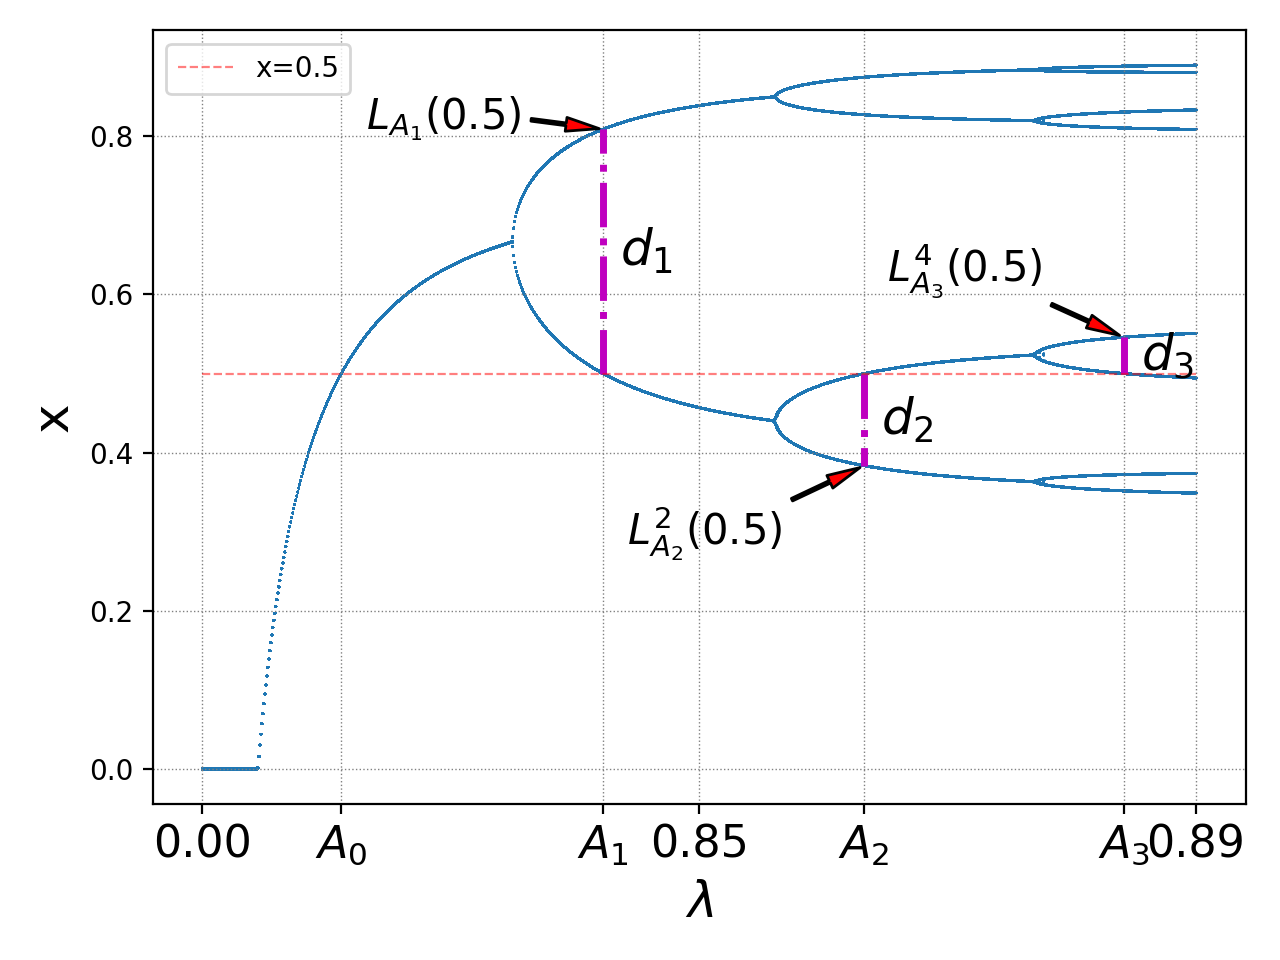
\includegraphics[width=0.8\textwidth]{./figures/demonstration of feigenbaum constants.png}
	\caption{ 
		A portion of the bifurcation diagram of the logistic map with demonstration of  $A_i$, which is the value of $\lambda$ at which the superstability of $2^i$ cycle is attained, and $d_i$, which is the distance between the superstability point (at $x=0.5$) and the closest point in the stable orbit.
		The $\lambda$ axis in in logarithmic scale, and the transformation to from $\lambda$ to $x$ coordinate is $-\log(A_{\infty} - \lambda)$.
	}
	\label{fig:demonstration of feigenbaum constants on logistic map}
\end{figure}

It is worthwhile to describe our algorithm to compute $A_i$ and $d_i$ in detail, as such seemingly innocuous computation is actually surprisingly challenging.
As for as the authors' knowledge, computations of $A_i$ to such precision has not been performed previously, and the method described here is original.

The first challenge is the precision of floating point arithmetic.
At $n = 10$, the value of $A_{n+1} -A_{n} $ is smaller than $ 10^{-8}$. 
To compute $\frac{A_{n+1} - A_n}{A_{n+2} - A_{n+1}}$ to $8$ significant figures (base 10), therefore, would require calculating $A_i$ to 16 significant figures, greater than the precision of the double precision floating point used in most computers, which only allows approximately 15 significant figures
\footnote{
	The IEEE standard for floating point arithmetic \cite{IEEE_floating_point} (IEEE 754) decrees 53 bits of binary digits in double precision floating point (page 8, table 3.2 of the standard.) This translates to $53 \cdot \log_{10}(2) \approx 15.8$ significant digits based 10.
}.
The only way to overcome this is to use an arbitrary precision arithmetic library. 
We chose to use GNU GMP (GNU Multiple Precision Arithmetic Library) \cite{GMP} with interface in C++.

The next challenge is the efficiency of the algorithm. 
If the algorithm starts by trying each $\lambda = 0$ and increments by $10^{-8}$ until $\lambda$ reaches $1$, the computer needs to compute literally billions of iterations of the logistic map, taking very long time and much wasted computer power.
The natural optimisation is to guess approximately where $A_i$ shall be and check $\lambda$ with greater precision in that area. 
In the process of guessing we still need to increment $\lambda$ by some difference, but initial increment of $\lambda$ can be relatively large, and whenever a value of $A_i$ is found, this difference shall be scaled down by Feigenbaum's  $\delta$.


While the full code in C++ was included in the appendix,
Algorithm \ref{ag:compute A_i} shows the pseudocode, which needs input parameters $\lambda_{start}$ for the start of $\lambda$, $\lambda_d$ for the initial increment of $\lambda$, and $n_{bound}$ for the maximum number of $A_i$ to be computed.
Algorithm \ref{ag:compute A_i} depends on Algorithms \ref{ag:super stable} and \ref{ag:fine tuning}. 
The former checks if superstability under a threshold is obtained at a certain $\lambda$, and the latter fine tunes $\lambda$ to obtain the most accurate value of $A_i$.
Both algorithms require various parameters including the threshold for superstability and the constant $c$ for fine tuning.
By poking different values for parameters of this algorithm, reasonably accurate numerics can be obtained up to $A_{15}$.


\begin{algorithm}
	\caption{Check if $\lambda$ is super stable}
	\begin{algorithmic}[1]
		\Require $\lambda$, cycle number $n,$ point of superstability $x^* = 0.5$, and threshold $t$.
		\If{$|L_{\lambda}^{2^{n-1}}(0.5) - 0.5| < t$}
		\State \Return True
		\Else
		\State \Return False
		\EndIf
	\end{algorithmic}
	\label{ag:super stable}
\end{algorithm}

\begin{algorithm}
	\caption{Fine Tuning $\lambda$}
	\begin{algorithmic}[1]
		\Require $\lambda$, cycle number $n,$ point of superstability $x^* = 0.5$, and an constant $c$. $\lambda \in (\lambda - c, \lambda +c)$ are checked.
		\State Create a list $L$ of $\lambda$ in the interval $I$.
		\State Compute the list $L^*$, which holds $L_{\lambda}^{2^{n-1}}(0.5)$ for each $\lambda$ in $L$.
		\State Set $\lambda$ to be the element in $L$ corresponding to the minimum value in $L^*$.
		\State Perform fine tuning by repeating the above steps after setting $c = c / \delta$. \Comment{$\delta$ is Feigenbaum's delta}
		\State Iteration stops when $c$ is smaller than a certain threshold.
	\end{algorithmic}
	\label{ag:fine tuning}
\end{algorithm}

\begin{algorithm}
	\caption{Computation of $A_i, d_i$}
	\begin{algorithmic}[1]
		\Require $\lambda = \lambda_{start}$, $A_i = \{0.5\}, d_i = \{\}$, and cycle number $n = 2$ (We have computed the first stability point is $0.5$, so we can start with cycle number $2$.)
		\While{$\lambda < \lambda_{end}$ and $len(A_i) < n_{bound} $}
		\If{$L_{\lambda}(0.5)$ is super stable}  \Comment{Using algorithm \ref{ag:super stable}}
			\State Fine tuning $\lambda$ with algorithm \ref{ag:fine tuning}.
			\State Append $\lambda$ to $A_i$ 
			\State Append $\L^{2^{n-1}}(0.5)$ to $d_i$ 
			\State $\lambda = \lambda + \lambda_{i}$
			\State $\lambda_{d} = \lambda_d / \delta$  \Comment{$\delta$ is Feiganbaum's delta}
			\State $\lambda_{i} = \lambda_i / \delta$
			\State $n = n + 1$
		\EndIf
		\State $\lambda = \lambda + \lambda_d$
		\EndWhile
	\end{algorithmic}
	\label{ag:compute A_i}
\end{algorithm}

\section{Single Nodal Functions Give Rise to Bifurcations}

Our previous discussion of infinite bifurcations of the logistic map is qualitative and the proof of Theorem \ref{th:logistic_bifurcation} only relies on the facts that the logistic map is differentiable, concaves downwards, has a unique maximum, and has negative Schwarzian derivative. 
It may not be of surprise, therefore, that the dynamical properties of bifurcation are shared among a large class of functions with very moderate restrictions.
Let us investigate some more examples.

Figure \ref{fig:combined_bifurcations} shows the bifurcation diagrams of $f(\lambda, x) = \lambda \sin(2\pi x)$, $f(\lambda, x) = \lambda + \sin(2\pi x)$, $f(\lambda, x) = \lambda x(1-x)^2$, and $f(\lambda, x) = \lambda x \log(x)$.
Infinite bifurcation and periodic doubling to chaos were observed for all cases, although the exact values of $\lambda$ at which the bifurcation take place is different for each map.
It is also striking that the shape of each bifurcation diagram is extremely similar to that of the logistic map up to elongation and stretching, so it is reasonable to conjecture that most of the points of Theorem \ref{th:logistic_bifurcation} shall also apply to these functions.
Indeed, point \ref{log_cross_half} of Theorem \ref{th:logistic_bifurcation} is readily demonstrated by Figure \ref{fig:combined_bifurcations}
as, in each subfigure, the horizontal line at the local maximum crosses the stable orbits of any periods at some $\lambda$.

% TODO: How shall we name these diagram if there is no bifurcation?
Figure \ref{fig:combined_no_bifurcations} shows the bifurcation (or the lack of bifurcation) diagrams of $\lambda \sin(2\pi x)$, $\lambda + \sin(2\pi x)$, $\lambda x(1-x)^2$, and $\lambda x \log(x)$. 
Each of these functions exhibit dynamical behaviour different from periodic bifurcations.
The $\lambda e^x$ map bifurcated precisely once at $-e$. 
For all $\lambda < -e$ there are two stable orbit, while for $\lambda > -e$ there are one stable orbits.
As for the tent map, there is one unique stable fixed point $x=0$ for $\lambda \in [-0.5, 0.5]$, and for any other $\lambda$ there seems to be no stable orbits at all but homogeneous region of chaos. 
The fact that tent map is chaotic is proved in Example \ref{ex:logistic and tent}.
The two $\arctan$ maps have similar behaviours to the exponential map. 
Their stable orbit only bifurcated once over all $\lambda \in \bb{R}$.

Why do the former class of functions exhibit infinite bifurcations to chaos, but the latter class do not?
The graphs of these functions, shown in Figure \ref{fig:combined_bifurcations_functions_graph}, may give the answer. 
All functions which give rise to bifurcations are smooth and have single-modal structures; that is, their values are bounded and attain unique maximums in some interval. Those which do not exhibit bifurcation are either not differentiable at the maximum, e.g. the tent map, or do not have local maxima, e.g. the exponential and arctangent maps.
This observation fits our expectation, as in the proof of Theorem \ref{th:logistic_bifurcation}, the most important property used is the fact that the logistic function attains a unique, differentiable maximum at $x=0.5$ and it concaves downwards. 
Metropolis et al. \cite{metropolis2017finite} have shown that the bifurcation phenomenon is universal, as summarised in the following theorem.

\begin{thm}[Criterion for infinite bifurcations]\label{th:criteria_for_infinite_bifurcations}
	If $f(x)$ satisfies the following properties:
	\begin{enumerate}
		\item $f(x)$ is continuous, singled valued, piecewise $C^1$ and has a unique differentiable maximum on the interval $[0,1]$ attained at $x^*$;
		\item $f(x) > 0$ on $(0,1)$, $f(0) = f(1) = 0$, and $f$ is strictly increasing in $[0, x^*]$ and strictly decreasing in $[x^*, 1]$;
		\item for $\Lambda_0 < \lambda < 1, \lambda f(x)$ has two fixed points (one of which is $x = 0$) both of which are repellent, that is $|\lambda f'(x)| > \frac{1}{\lambda}$; and,
		\item in the interval $N$ around the unique maximum $f$ concaves down-wards,
	\end{enumerate}
	then the system $x_{n+1} = \lambda f(x_n)$ will exhibit infinite bifurcations and periodic doubling to chaos.
	To be precise, the criterion for chaos by period doubling bifurcations is:
	\begin{enumerate}
		\item for $\Lambda_0 < \lambda < \lambda_{\infty} < 1$, there exists stable orbit of period $2^n$ for all $n = 1, 2, \cdots$. with $n$ increasing with $\lambda$; and
		\item for each $\lambda$, there exists at most one set of stable orbits.
	\end{enumerate}
\end{thm}

\begin{figure}
	\centering
	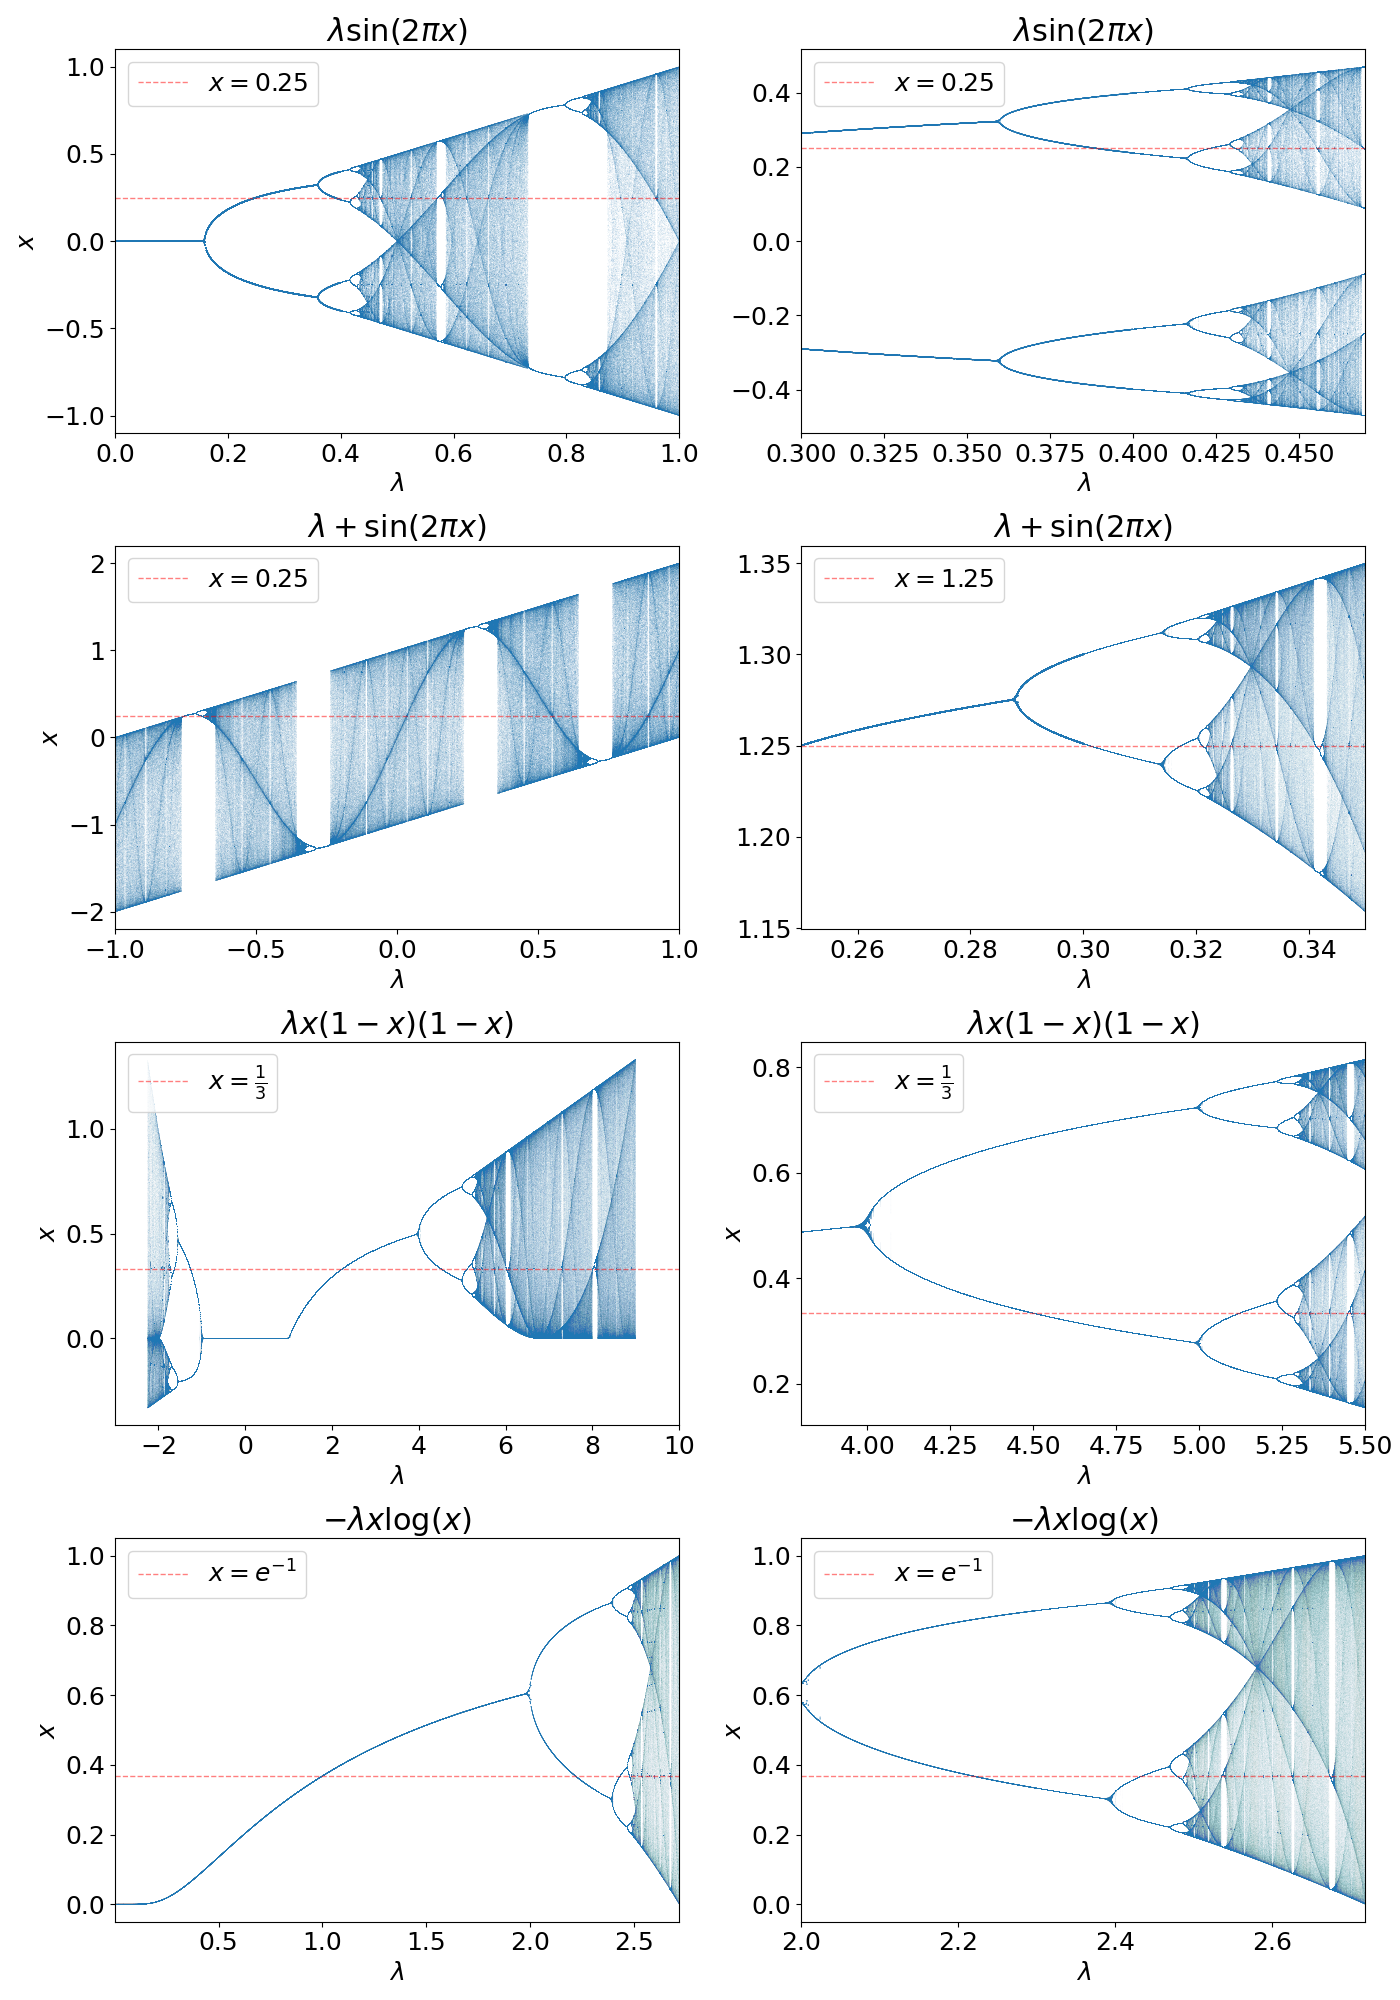
\includegraphics[width=\textwidth]{./figures/combined_bifurcations.png}
	\caption{
		Bifurcations diagrams of four different functions 
		$ \lambda \sin(2\pi x)$,
		$ \lambda + \sin(3\pi x)$,
		$ \lambda x(1-x)^2$,
		and $ \lambda x \log(x)$.
		All of these functions exhibit bifurcations and periodic doubling to chaos like the logistic map. 
		The subfigures on the left are the overview of bifurcations, where the ones on the right are zoomed in around points of bifurcation.
		The graph of these functions are presented in Figure \ref{fig:combined_bifurcations_functions_graph}
	}
	\label{fig:combined_bifurcations}
\end{figure}

\begin{figure}
	\centering
	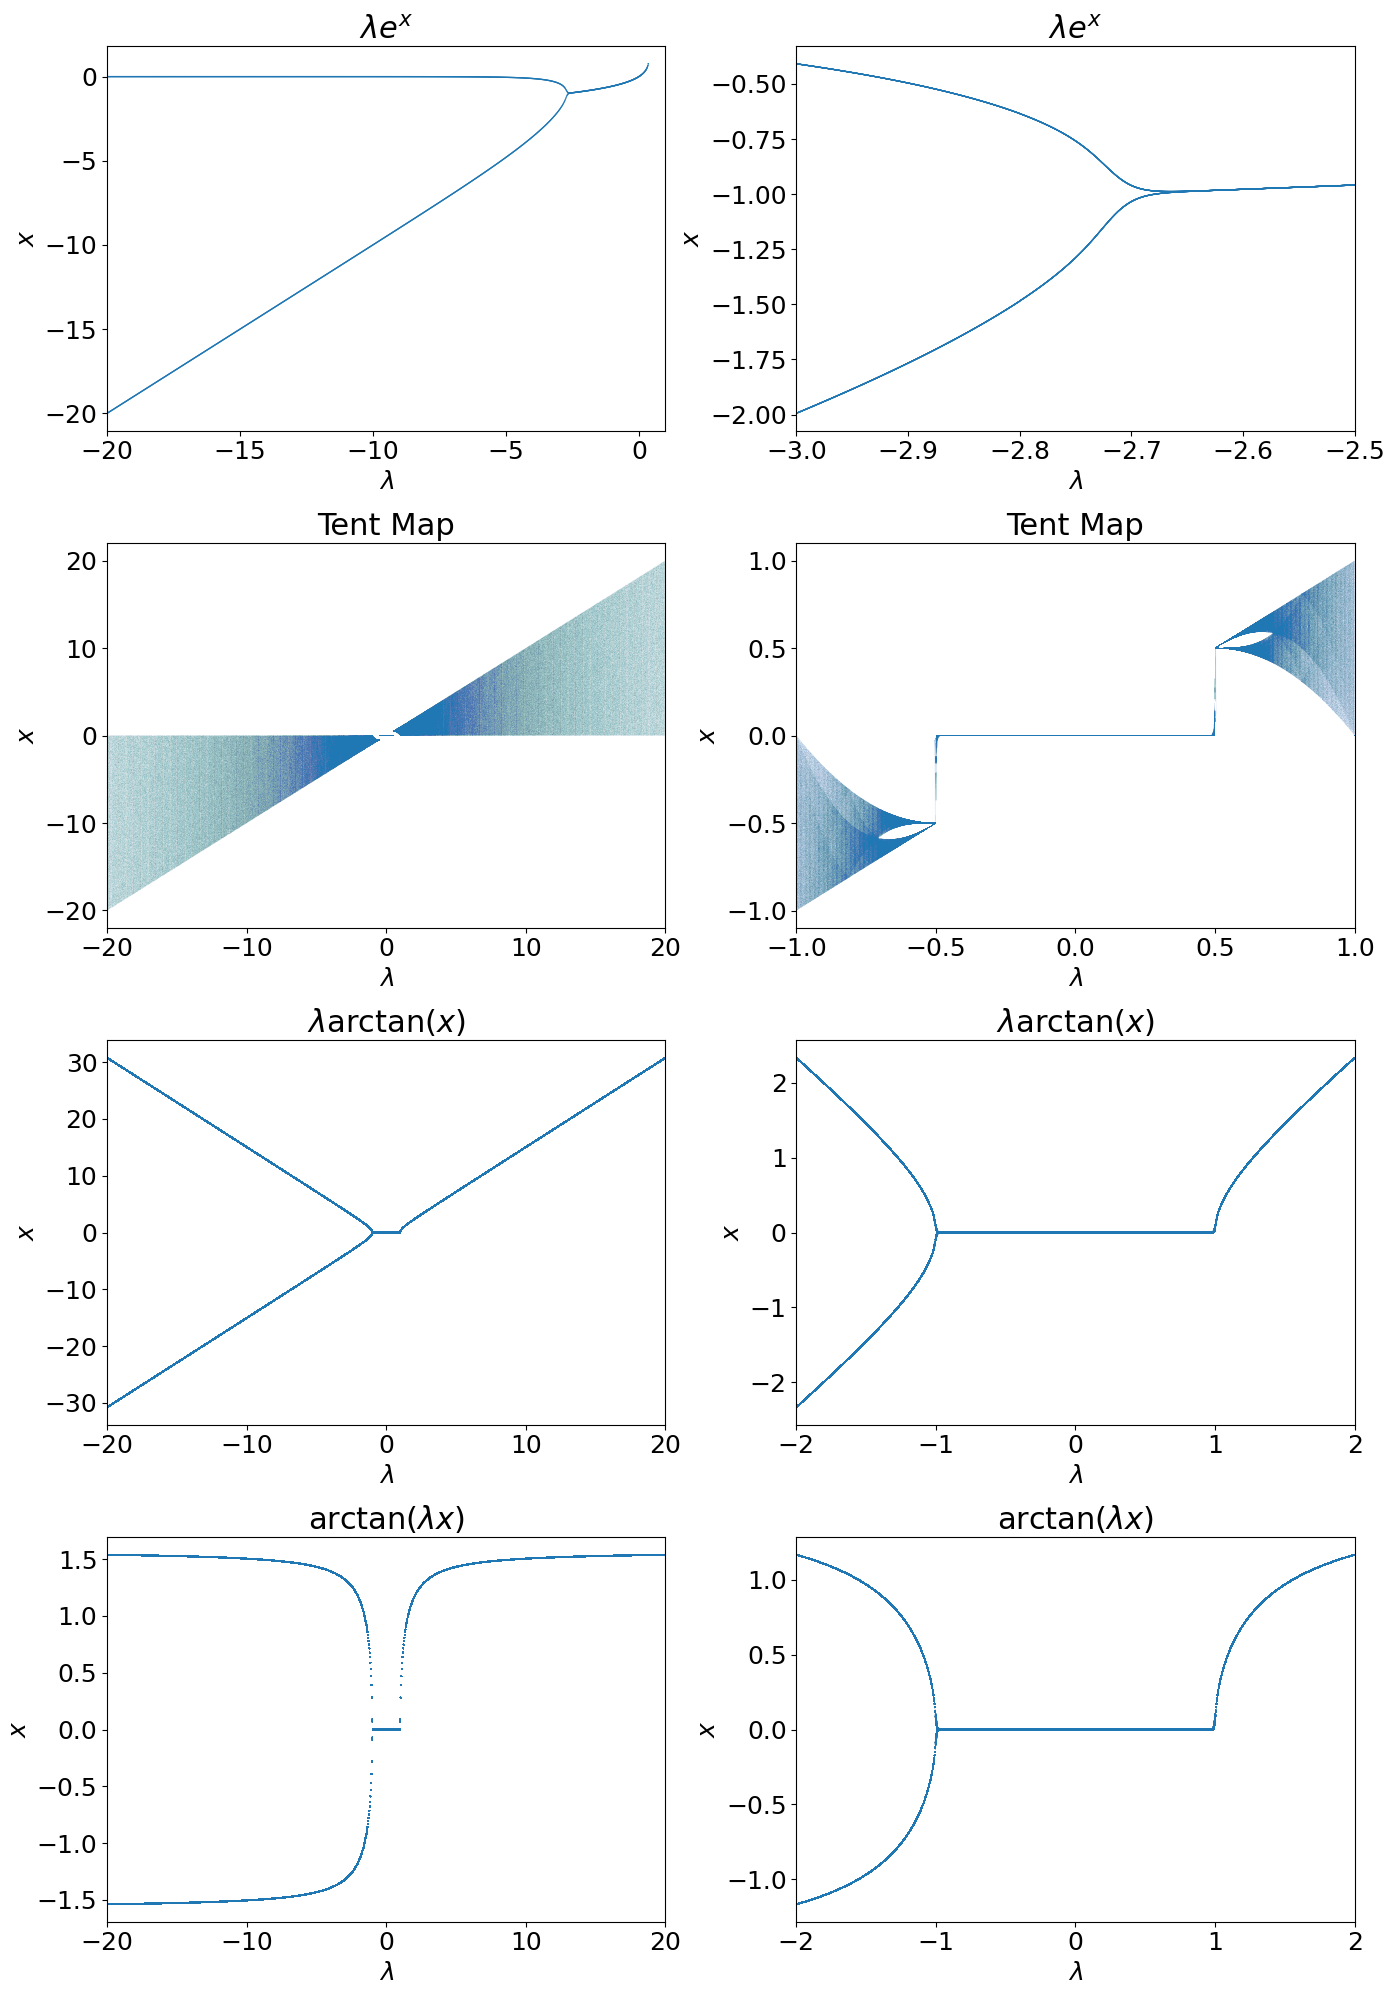
\includegraphics[width=\textwidth]{./figures/combined_no_bifurcations.png}
	\caption{
		These figures show patterns of (or lack of) stable orbits for four functions which do not exhibit periodic doubling to chaos. 
		The graph of these functions were presented in Figure \ref{fig:combined_bifurcations_functions_graph}.
	}
	\label{fig:combined_no_bifurcations}
\end{figure}

\begin{figure}
	\centering
	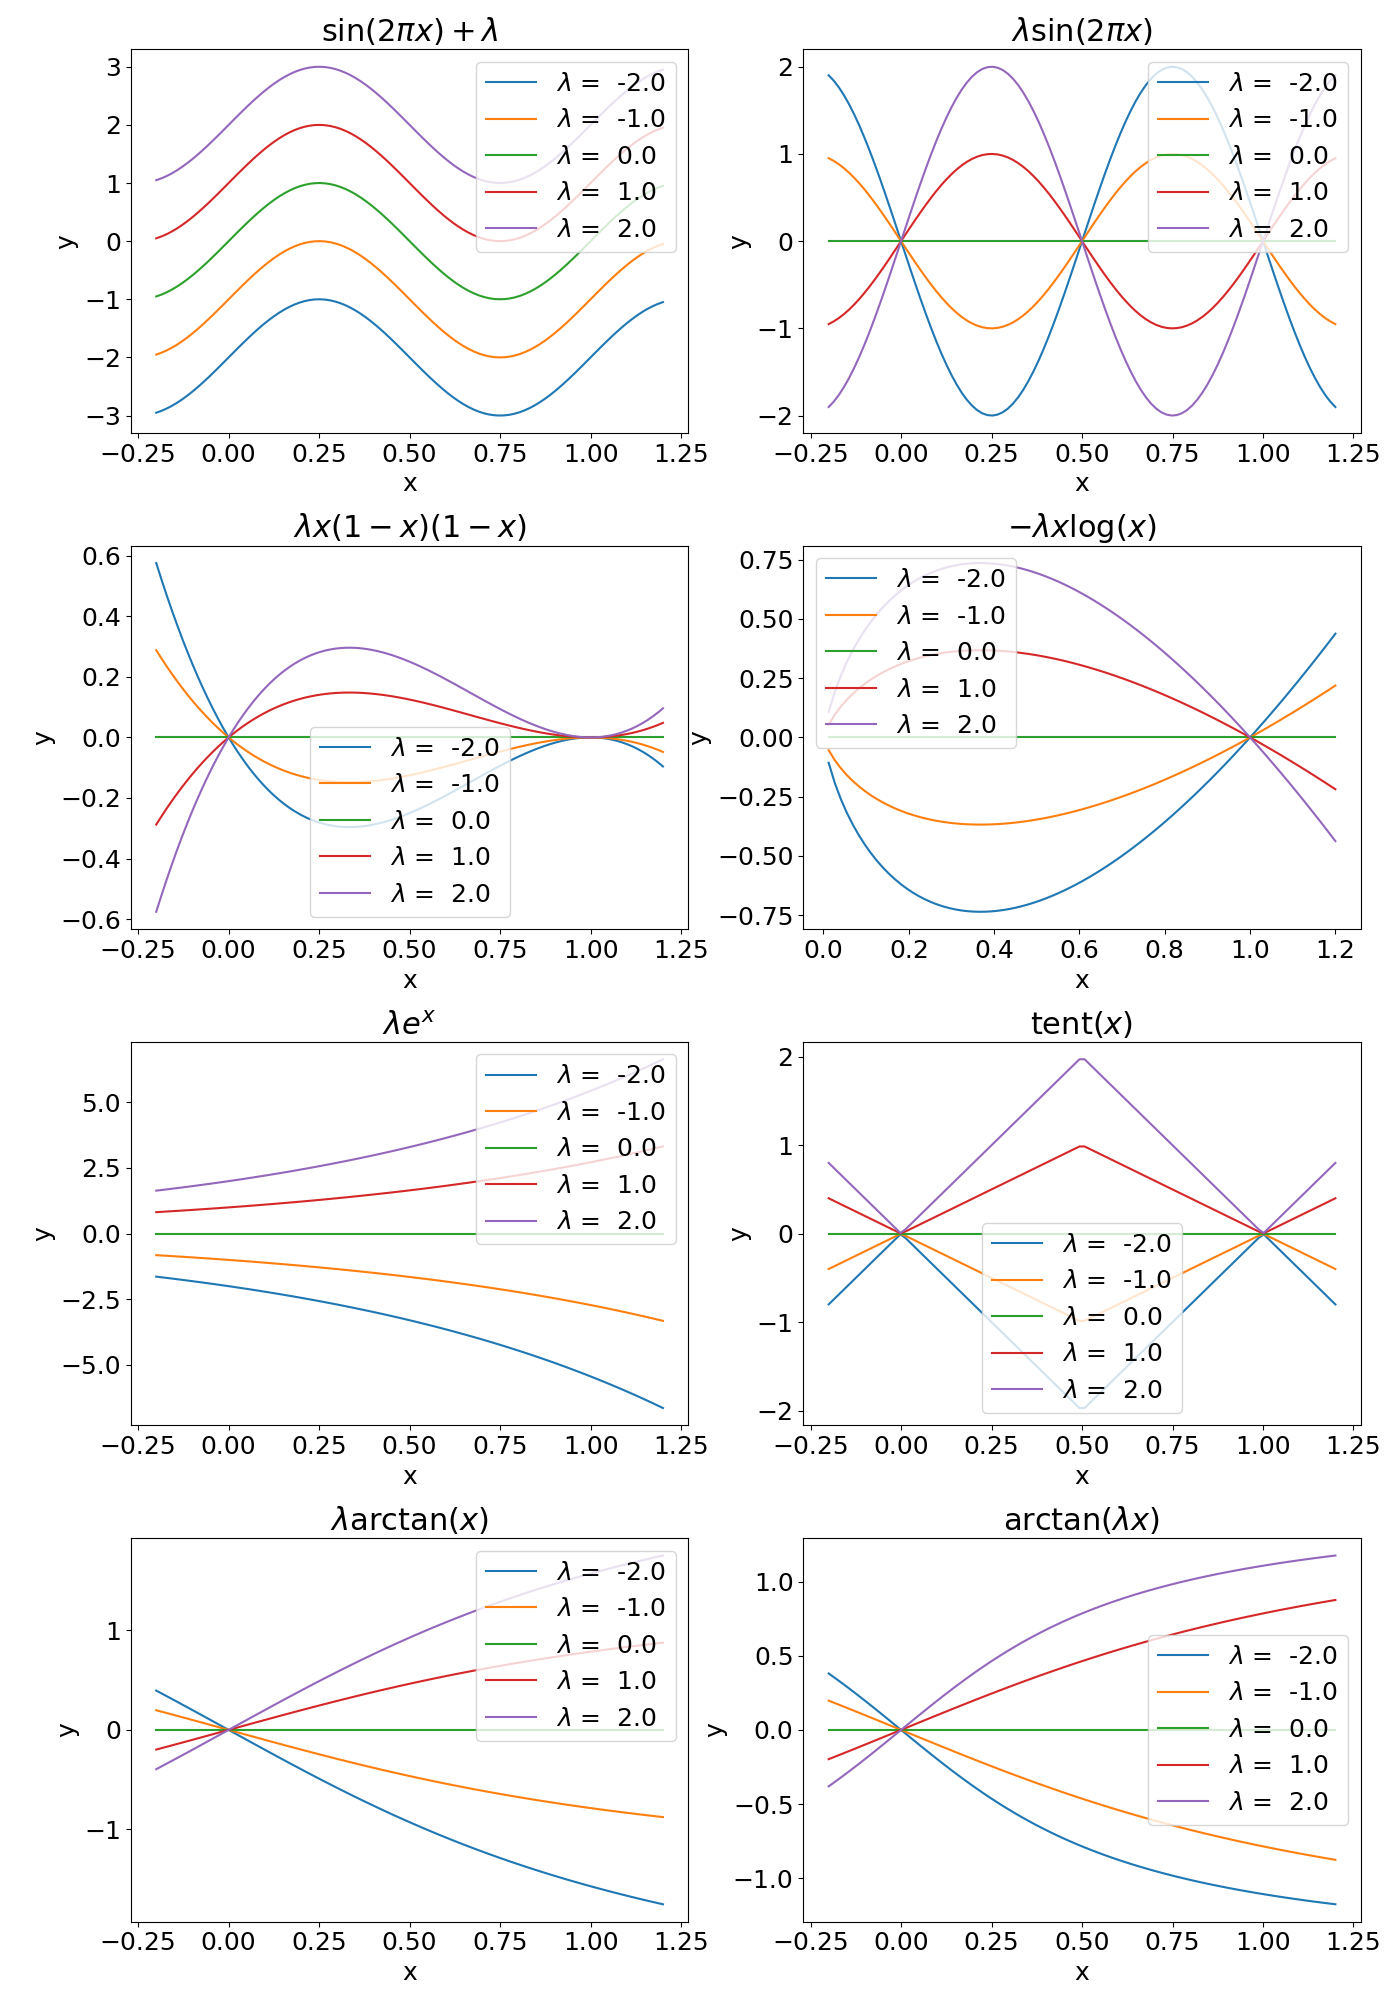
\includegraphics[width=\textwidth]{./figures/combined_functions.png}
	\caption{
		This figure shows the graph of the functions whose bifurcation diagrams are graphed on Figure \ref{fig:combined_bifurcations} and \ref{fig:combined_no_bifurcations}.
	}
	\label{fig:combined_bifurcations_functions_graph}
\end{figure}


Having settled that the periodic bifurcation is a universal phenomenon for a large class of functions, naturally we ask how about the scaling constants shown in Table \ref{tab:feigenbuam_alpha_table_for_logistic}.
The surprising fact is that Feigenbaum's constants $\delta$ and $\alpha$ are universal for any iterative map depending on one variable and exhibit periodic doubling bifurcations with orbit $2^0, 2^1, 2^2, \cdots$. 
Indeed, Tabor showed that such constants are universal for iterative maps with negative Schwarzian derivative \cite{Tabor}.
The entirety of the last chapter will be dedicated to the demonstration of this fact based on Feigenbaum's theory of scaling. 
Here, instead, we present another numerical evidence for the universality of Feigenbaum's constants.

Table \ref{tab:feigenbuam_constants_skewed_logistic_map} shows the $A_i$, $d_i$, and their ratios for the skewed logistic map $f_{\lambda} (x) = \lambda x (1-x)^2$.
The numerics were calculated with an algorithm similar to Algorithm \ref{ag:compute A_i}.
Although the speed of convergence is clearly different, 
$ \frac{d_n}{d_{n+1}} $ and $\frac{A_{n+1} - A_n}{A_{n+2} - A_{n+1}}$ seem to converge to the same number as in the logistic map.
\begin{table}
\centering
\begin{tabular}{|c|c|c|c|c|}
\hline
\( n \) & \( A_n \) & \( d_n \)  & \(\frac{A_{n+1} - A_n}{A_{n+2} - A_{n+1}}\)  &  \(\frac{d_n}{d_{n+1}}\) \\ \hline
0 & 2.25000000 & - & 3.58291025 & - \\
1 & 4.49325749 & 0.33233444 & 4.41239995 & 3.11334650\\
2 & 5.11935677 & 0.10674508 & 4.60351732 & 2.31871272 \\
3 & 5.26125217 & 0.04603635 & 4.65268653 & 2.58607785 \\
4 & 5.29207543 & 0.01780161 & 4.66307535 & 2.47302222 \\
5 & 5.29870026 & 0.00719832 & 4.65793977 & 2.51729830 \\
6 & 5.30012096 & 0.00285954 & 4.67119534 & 2.49830019 \\
7 & 5.30042596 & 0.00114459 & 4.64986027 & 2.50813287 \\
8 & 5.30049126 & 0.00045635 & 4.65947170 & 2.50369628 \\
9 & 5.30050530 & 0.00018227 & 4.66753118 & 2.50386731 \\
10 & 5.30050832 & 0.00007279 & 4.66237768 & 2.50460649 \\
11 & 5.30050896 & 0.00002906 & 4.64855560 & 2.50672818 \\
12 & 5.30050910 & 0.00001159 & 4.65083889 & 2.50600317 \\
13 & 5.30050913 & 0.00000462 & 4.66534446 & 2.50451859 \\
14 & 5.30050914 & 0.00000184 &  - & 2.50767228   \\
15 & 5.30050914 &  0.00000073&  - &  - \\
\hline
\end{tabular}
\caption{
	Values of \( A_n \), \( \delta_n \), and their ratios up to ten decimal places for the skewed logistic map $f_{\lambda}(x) = \lambda x(1-x)^2$.
	The calculations are the same as in Table \ref{tab:feigenbuam_alpha_table_for_logistic}.
}
\label{tab:feigenbuam_constants_skewed_logistic_map}
\end{table}

\chapter{Feiganbaum's Theory of Scaling}
\section{Feigenbaum's Theory of Scaling}

The whole of bifurcation theory is spectacular; even more amazing are the Feigenbaum constants $\alpha$ and $\beta$, whose existence and universality are demonstrated by the numerics in table \ref{tab:feigenbuam_alpha_table_for_logistic} and \ref{tab:feigenbuam_constants_skewed_logistic_map}.
The proof that these constants exist and are universal is well beyond the scope of this undergraduate project, but we can give some rational argument as to the existence of $\alpha$.

\begin{figure}
    \centering
    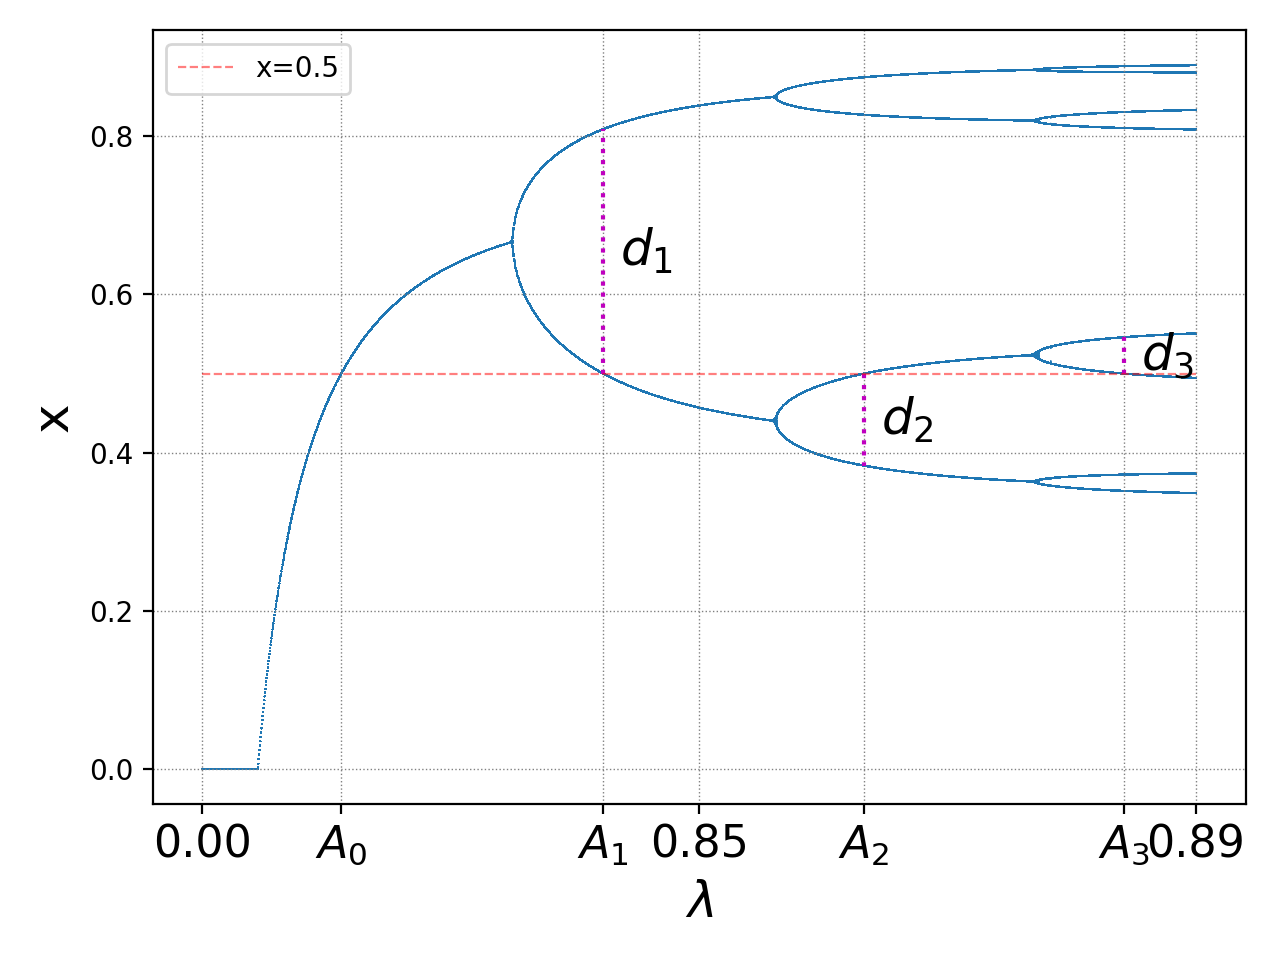
\includegraphics[width=0.6\linewidth]{Images/demonstration of feigenbaum constants.png}
    \caption{Bifurcation diagram of the logistic map which shows the location for $A_n$ and $d_n$ for the first 3 period doubling bifurcations.}
	\label{fig: universal raito}
\end{figure} 

Recall that $\alpha = \lim_{i \rightarrow  \infty}\frac{b_i}{b_{i-1}}$. 
For a given iterative map $F$, depending on one parameter satisfying the requirement of \ref{th:criteria_for_infinite_bifurcations}, $b_i$ is the distance at the superstability of the $2^{i}$ cycle between $X_{m}$ and its closest point in the cycle, where $X_m$ is the unique maximum of $F$.

Writing it in another way
\begin{equation}\label{eq:d_sim}
d_r \sim\frac{D}{(-\alpha)^r} \quad \quad \text{ as } r \to \infty
\end{equation}
where $D$ is a constant depending on $F$ and $\alpha$ is the Feigenbaum's constants. 

Theorem \ref{th:logistic_bifurcation}.\ref{log_closest_branch} states that $d_i = F^{2^{n-1}}(A_i, X_m) - X_m$, where $A_i$ is the value of the parameter at which the $2^n$ cycle achieves superstability and crosses $X_m$ (see figure \ref{fig: universal raito}). 
Therefore, to find the scaling of $d_r$, we take the limit of \eqref{eq:d_sim},

\begin{equation}
\lim_{r \to \infty} (-\alpha)^r \left(F^{2^r}(A_{r+1}, X_m) - X_m\right) = - \frac{D}{\alpha}.
\end{equation}

This leads to the hypothesis that
$$
g_1(x-X_m)=\lim_{r \to \infty} \{g_{1r}(x-X_m)\},
$$
where
$$
g_{1r}(x-X_m) = (-\alpha)^r \{F^{2r}(A_{r+1}, X_m + (x-X_m)/(-\alpha)^r)-X_m\}.
$$
Let $x-X_m$ be the difference from the point of superstability about the bifurcation to $X_m$. 
From the scaling of $d_r$, this implies that $g_1(0)=-\frac{D}{\alpha}$ and by solving for the first couple of iterations of $g_{1r}(x-X_m)$, we can see a limit emerge for $g_1$.
Feigenbaum said that $g_1$ is dependent on the scaling of $x-X_m$ which shows the behaviour of $F$ near to its maximum. 
Since $g_1$ doesn't matter on the map $F$ we can thus say that this behaviour causes $g_1$ to become universal.

Without loss of any generality we can set $X_m=0$.
The main ideas of scaling $x$ can be seen by the operator $T$, which we define to be
\begin{equation} \label{eq: operator T}
T\psi(x)=-\alpha \psi (\psi(-\frac{x}{\alpha})),
\end{equation}
for all continuous functions $\psi$.
Setting $\psi=g_1$, we have
\begin{align}
    Tg_1 &=-\alpha g_1(g_1(-x/\alpha)) \nonumber \\
    &= -\alpha \lim_{r \to \infty} \{(-\alpha)^rF^{2r}(A_{r+1}, (-\alpha)^rF^{2r}(A_{r+1},x/(-\alpha)^{r+1}))\}.  \label{eq:one}
\end{align}
Now, if we set $\phi(y)=(-\alpha)^rF^{2r}(A_{r+1},y/(-\alpha)^r))\}$ such that $$\phi^2=\phi(\phi(y))=(-\alpha)^rF^{2r+1}(A_{r+1},y/(-\alpha)^r))\}$$ and $y=\frac{x}{\alpha}$, we can see that
\begin{align*}
    Tg_1 &= \lim_{r \to \infty} \{(-\alpha)^{r+1}F^{2r+1}(A_{r+1}, x/(-\alpha)^{r+1})\} \\
    &= \lim_{q \to \infty} \{(-\alpha)^qF^{2q}(A_q,x/(-\alpha)^q)\} \\
    &= g_0(x)
\end{align*}
This then implies that $Tg_k(x)=g_{k-1}(x)$ for $k = 2,3,...$ where we have shown that,
\begin{align}
    g_k=\lim_{r \to \infty} \{(-\alpha)^{r}F^{2r}(A_{r+k}, x/(-\alpha)^{r})\}. \label{eq:two}
\end{align} 
As $k \to \infty$ we can show that there could exist a function $g(x)= \lim_{k \to \infty}g_k(x)$ such that we can create the functional equation,
\begin{align}
    Tg=g \label{eq:FunctionalOperator}
\end{align}
such that we can say there exists a `fixed point' $g$ of the nonlinear functional operator $T$. This tells us that when we apply $T$ to $g$, this doesn't change the inherent properties of $g$. 

Using the functional equation \eqref{eq:FunctionalOperator}, the constant $\alpha$ must be determined as part of the solution. The function $g(x)$ satisfies this functional equation, and it possesses a scaling symmetry, such that if $g(x)$ is a solution, then the rescaled function $\mu g(x/\mu)$ is also a solution for any $\mu \neq 0$. This scaling symmetry implies that there is an inherent freedom in the choice of the parameter $\mu$, meaning the solution is not unique until this freedom is constrained. To fix $\mu$ and ensure a unique solution, we adopt a convention by selecting a specific value of $\mu$ such that the function $g(x)$ satisfies a normalisation condition. Once this value of $\mu$ is chosen, the functional equation determines the value of the constant $\alpha$. Although $\alpha$ can be obtained numerically through the solution of the difference equations, its formal derivation comes from solving the functional equation under the chosen normalisation. Thus for the function $g(x)$ that corresponds to the desired map, we can choose a particular $\mu$ such that,
$$
g(0)=1
$$
and by setting $x=0$ in the functional equation and via the original definition of our operator we have it that,
$$
\alpha = -1/g(1)
$$

Feigenbaum was able to numerically verify the method, where he found that
\begin{align}
    g(x)= 1 - 1.52763x^2 + 0.10482x^4- 0.02671x^6 + \dots .\label{eq:feigenbaum}
\end{align}
that corresponds to the desired $\alpha =-1/g(1)=2.5029$.

\begin{exmp} The Logistic Map

    For the logistic map, we have that $F(a,x)=ax(1-x)$ such that the maximum value is attained at $X_m =1/2$. Thus we are able to replace $x-X_m$ with $x-1/2$. Hence our new function is given as $F(a,x)=a(1/4-x^2)-1/2$, ensuring that the maximum value of our new function occurs at $x=0$. Using equations \eqref{eq:one} and \eqref{eq:two} we can now see that,
    \begin{align}
        g_{10}&=F(A_1,x)=A_1(1/4-x^2)-1/2 \nonumber \\
        g_{11}&=(-\alpha)F^2(A_2,x/(-\alpha)) \nonumber \\
        &= \alpha A_2 \left(\left(A_2 \left(x^{2}/\alpha^2 - 1/4\right) + 1/2\right)^{2} - 1/4\right) + \alpha/2
    \end{align}
    Thus, for $g_{1r}(x)$, we can plot our findings as $r \to \infty$ in the $x, y$ plane where $y=g_{1r}(x)$. 
	When we present our first couple of plots, we can see a clear limiting function $g_{k=1}$ appearing as $r$ increases. Thus from \eqref{eq:two} we can see that, as we increase $k$, the sequence of functions converges to some function $g(x)$. 
	We can see the behaviour of our results in the plots in Figure \ref{fig:unscaled}.
	\begin{figure}
    \centering
    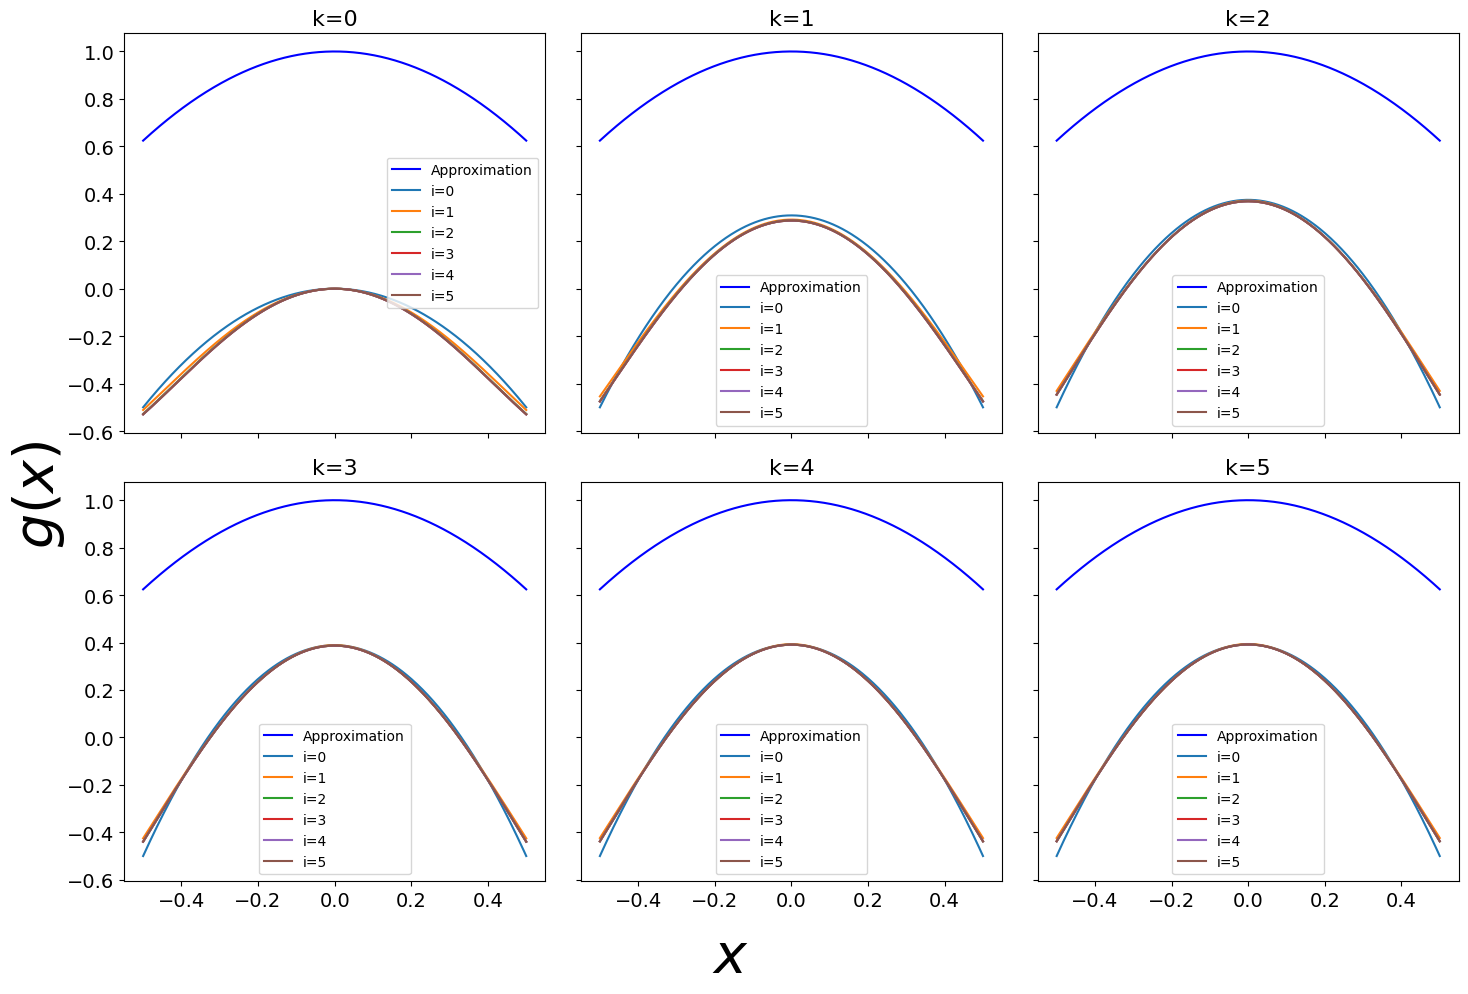
\includegraphics[width=1\textwidth]{Feigenbaum Approx Graphs/Images/feigenbaum.png}
    \caption{Unscaled graphs corresponding to the logistic map}
    \label{fig:unscaled}
\end{figure}
    

    The blue line shows us Feigenbaum's numerically solved solution \eqref{eq:feigenbaum} while the rest of the lines show us the iterations of $r$ for specified $k$ values. 
	We can see that our results produce a correct solution; as we iterate $r$, we can see that our plots converge. However, we can clearly see that our plots don't converge to the desired solution found by Feigenbaum \eqref{eq:feigenbaum}. Since we know, by the universality of the approach, that there exists a scaling factor. From the non linear function operator \eqref{eq:FunctionalOperator}, there exists some scaling factor $\mu$. Thus our solution corresponding to the logistic map has an equivalent solution that matches the one found by Feigenbaum. Since we know $g(0)=1$, we have that $Tg(0)=\mu g(0)$ implies $\mu = 1/g(0)$, where $g(0)$ here is our map's solved unscaled value at 0. From our findings, we found that our value of $g(0)$ is $0.39176186028018406$ such that the corresponding scaling factor was found to be $\mu= 2.552571093277968$. Now that we have our new rescaled function $g(x)$, we can plot the iterations of $r$ and $k$. The results are shown in Figure \ref{fig:rescaled}.
    \begin{figure}
    \centering
    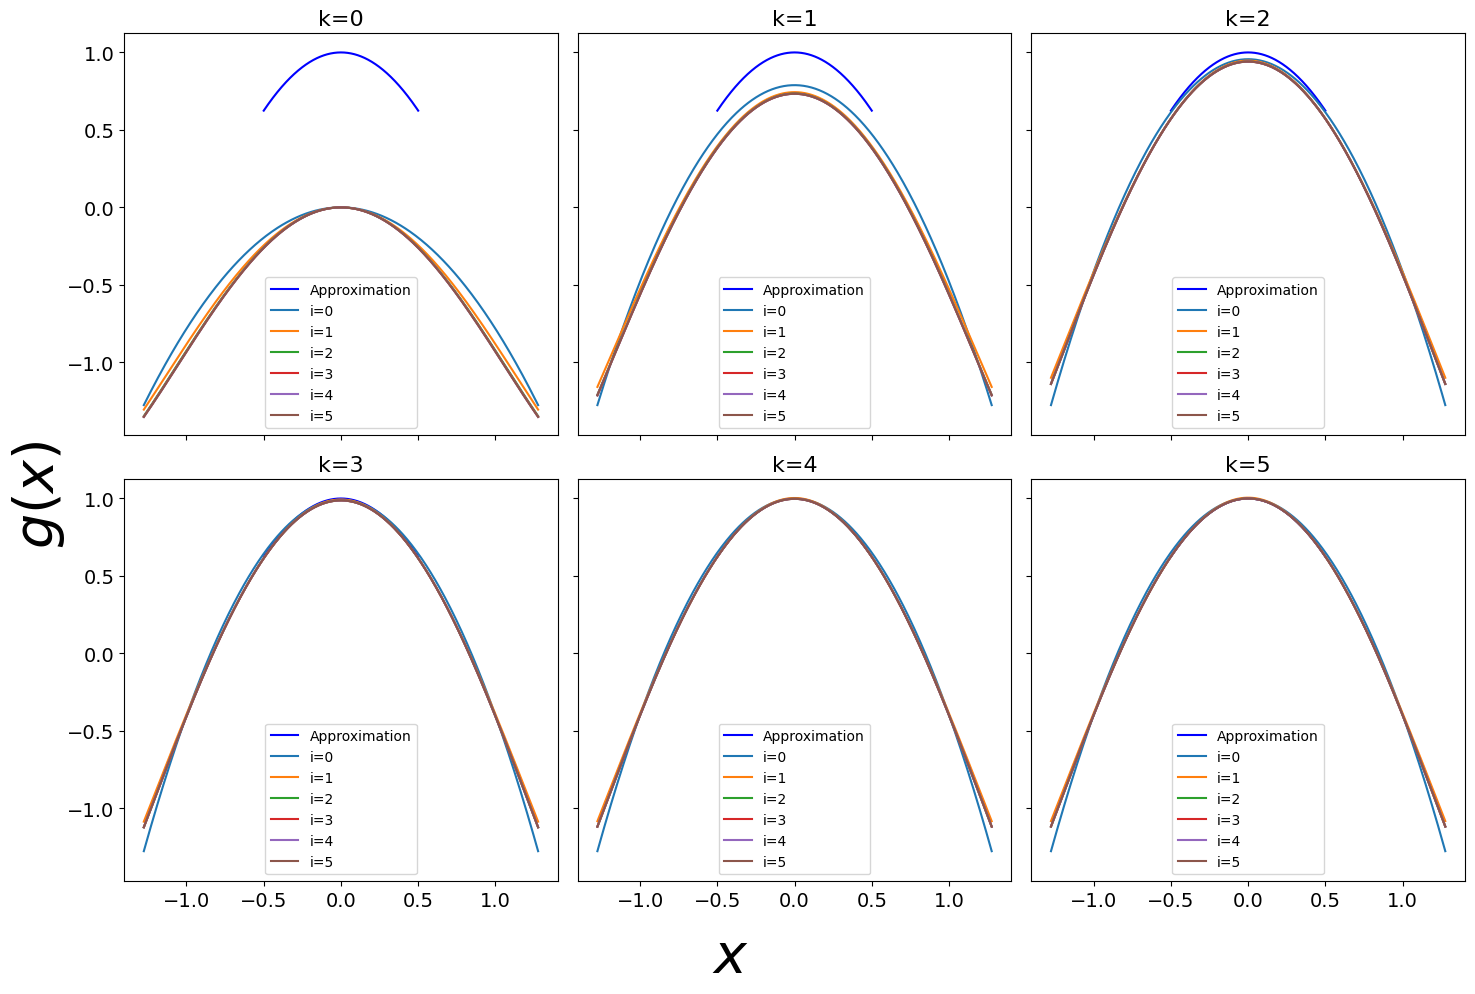
\includegraphics[width=1\textwidth]{Feigenbaum Approx Graphs/Images/fiegenbaum_scaled.png}
    \caption{Rescaled graphs corresponding to the logistic map}
    \label{fig:rescaled}
\end{figure}
The blue lines again show us Feigenbaum's numerically solved solution \eqref{eq:feigenbaum}. We can now see that due to $\mu$, our rescaled $g(x)$ now shifts up towards the true solution and attains the desired shape showing us that we have successfully rescaled our original solution to the universal one presented by Feigenbaum. Thus we have demonstrated the convergence described by Feigenbaum towards his numerical solution as well as the existence of a limiting function $g(x)$ as we increase both $r$ and $k$ simultaneously. 
\end{exmp}


\section{Numerical Computation of Eigenfunction of $T$}

To make the above section rigorous, and prove the existence of an eigenfunction of the operator $T$, is non-trivial and requires a hundred-page proof \cite{lyubich1999feigenbaum}, let alone finding such a function, and is clearly out of the scope of an undergraduate mathematical report like this one. 
In this section, we will attempt to compute the first few terms of the power series of this eigenfunction.

Assuming $g(0) = 1$ and that $g$ is an even function, (the validity of such assumption is justified by the fact that a successful result was found based on it), it can be written in the form of Taylor expansion 
$$
g = 1 + b_1 x^2 + b_2x^4 + \cdots 
$$
Defining the $n$th partial sum of this power series as $g = 1 + b_1x^2 + \cdots + b_{n-1}x^{2n-2}$, and applying $T$ to $g_n$ will produce another $(2n-2)^2$-degree polynomial whose coefficients depend on $b_1, \cdots, b_{n-1}$ and $\alpha$.
Ignoring the terms of degree higher than $2n-2$, and equating the coefficients of the result with that of $g$ of the same degree will give $n$ functions for $n$ variables, whose solution can be solved numerically. 

We will demonstrate an example for $g_1 = 1 + b_1 x^2$. 

Note 
$$
g_1(-\frac{x}{\alpha}) = 1 + b_1 \frac{x^2}{\alpha ^2}
$$

and, by plugging in,

\begin{align*}
-\alpha g_1(g(-\frac{x}{\alpha})) 
&= -\alpha( 1 + b_1(1+b_1 \frac{x^2}{\alpha^2})^2) \\
&= -\alpha(1 + b_1(1 + b_1^2\frac{x^4}{\alpha^4} + x^2 \frac{2b_1}{\alpha^2})) \\
&= -\alpha (1 + b_1)  - \frac{2b_1^2}{\alpha} x^2 - \frac{b_1^3}{\alpha^3}x^4
\end{align*}

thereby comes the equation 

$$
\begin{cases}
    1 &= -\alpha(1+b_1) \\
    b_1 &= -\frac{2b_1^2}{\alpha} 
\end{cases}
$$

The solution is $\alpha = 1 + \sqrt{3} \approx 2.732$ and $b_1 = - \frac{\sqrt{3}}{2} - \frac{1}{2} \approx -1.366$.

Calculating any more terms by hand would be an extremely tedious process, luckily we can resort to computer algebra system for symbolic manipulation (we used Sympy) and BLAS library (fsolve from Scipy) for solving equations of $n$ variables. 
The approximation for the fifteen term is shown in table \ref{tb:b_i table}.
The python code for producing these results is included in Appendix B.

\begin{table}
\centering
\begin{tabular}{|c|c|}
\hline
$n$ & $b_n$ \\
\hline
1 & \( -1.527632997 \times 10^{0} \) \\
2 & \( 1.048151948 \times 10^{-1} \) \\
3 & \( 2.670567058 \times 10^{-2} \) \\
4 & \( -3.527409767 \times 10^{-3} \) \\
5 & \( 8.160111810 \times 10^{-5} \) \\
6 & \( 2.528490972 \times 10^{-5} \) \\
7 & \( -2.556150238 \times 10^{-6} \) \\
8 & \( -9.664817874 \times 10^{-8} \) \\
9 & \( 2.828824961 \times 10^{-8} \) \\
10 & \( -3.352250769 \times 10^{-10} \) \\
11 & \( -2.716117768 \times 10^{-10} \) \\
12 & \( 1.171671302 \times 10^{-11} \) \\
13 & \( 7.447301044 \times 10^{-12} \) \\
14 & \( -2.868216370 \times 10^{-12} \) \\
15 & \( 9.052335129 \times 10^{-13} \) \\
\hline
\end{tabular}
\caption{The values of $b_n$ is the coefficients for the Taylor expression of $g$, where $g$ is the solution to $Tg = g$.
(That is $g = 1 + \sum_{i=1}^n b_i x^{2i}$)}
\label{tb:b_i table}
\end{table}

% \addcontentsline{toc}{chapter}{Conclusion}
\chapter*{Conclusion}
\addcontentsline{toc}{chapter}{Conclusion}
In this report, we identified chaotic dynamical systems, showing the consequences of the Lyapunov exponent on time-dependent functions. We proceeded to investigate quantifiable properties of these systems, motivated by an interest in the behaviour of such complicated dynamics. Throughout, we built theory and provided key examples of each topic in order to introduce and discover these properties. As well as this, we built our own computer code to assist with visualisations and numerical approximations, steps which, throughout history, have proven to be highly important in the study of dynamical systems. 

The crescendo of our report was in approximating the Feigenbaum constants; we were able to surpass Feigenbaum's numerical computations with the use of modern computer technologies and derive an approximation of the constants to a high degree of accuracy.
There are, of course, room for improvement of numerical accuracy, which will necessarily require truly ingenious algorithms and mastery of programming techniques. 
It would be suitable for an undergraduate project for future generations.

The field of chaotic dynamical systems is vast and spectacular, and this report has but touched the very surface. 
There are countless questions to be asked. 
What are the analytical properties of the Feigenbaum constants? 
Are they rational, irrational, or transcendental? 
Do they have a closed form or any relationship with other fields of mathematics?
This report has only investigated the Feigenbaum constants corresponding to the periodic doubling bifurcations of discrete dynamical systems of one parameter. 
Periodic bifurcation of triple and higher multitudes, and that of more parameters and continuous systems, are known to exhibit similar behaviours and can be described by other universal constants. 
How to generalise the methods in this report to these more complicated systems? What would these constants be, and how do they relate to each other?
They will constitute interesting topics for future research well beyond the scope of an undergraduate project.


% \bibliographystyle{...} 
\printbibliography
\addcontentsline{toc}{chapter}{Bibliography}

\begin{appendices}
	\chapter{Numerical Calculations for Point of Super-stability}
	This chapter includes our C++ code for numerical calculations of points of superstability for the logistic and skewed logistic maps.

The code was written in C++, compiled with g++ (GCC) 14.2.1 20250128, using GNU MP library version 6.3.0, and is shown below. 

It is also available at \url{https://github.com/quantifying-chaos/graph_qc/blob/main/cpp/numerical_feigenbaum_constants/main.cpp}.

% including the code 
\begin{lstlisting}[style=cppstyle]
// compile with -lgmpxx -lgmp
#include <algorithm>
#include <bits/stdc++.h>
#include <chrono>
#include <cmath>
#include <gmp.h>
#include <gmpxx.h>
#include <iomanip>
#include <iostream>
#include <stdexcept>
#include <vector>

#define PRECISION 4096 // in bits

using namespace std;

typedef void (*iter_map)(mpf_class &, mpf_class, mpf_class);
typedef mpf_class (*mpf_func)(mpf_class);

const mpf_class ALPHA = mpf_class(2.503, PRECISION);
const mpf_class DELTA = mpf_class(4.669, PRECISION);

template <typename T> void display(vector<T> &dis) {
  for (auto i : dis) {
    cout << i << endl;
  }
  cout << "length: " << dis.size() << endl;
}

mpf_class random_mpz(long low, long high) {
  if (high <= low) {
    throw std::invalid_argument(
        "high must be greater than low in random_mpz!");
  }
  static gmp_randclass r1(gmp_randinit_default);
  static int init = 0;
  if (!init) {
    r1.seed(std::chrono::system_clock::now()
                .time_since_epoch()
                .count());
    init = 1;
  }

  return low + r1.get_f() * (high - low);
}

void logistic(mpf_class &res, mpf_class lambda,
              mpf_class x) {
  res = 4 * lambda * x * (1 - x);
}

void logistic_skewed(mpf_class &res, mpf_class lambda,
                     mpf_class x) {
  res = lambda * x * (1 - x) * (1 - x);
}

// Iterate the functions n times, with input x and parameter
// lambda, and set the res to the result. the input map must
// have signature like logistic that is, void map(mpf_class
// &res, mpf_class lambda, mpf_class x)
void iterate(mpf_class &res, iter_map map, unsigned int n,
             mpf_class lambda, mpf_class x) {
  res = x;
  for (unsigned int i = 0; i < n; i++) {
    map(res, lambda, res);
  }
}

bool is_super_stable(
    iter_map map, mpf_class (*x_bar)(mpf_class),
    mpf_class lambda,
    unsigned int
        orbit_2_power, // at lambda, map has a stable
                       // 2^orbit_2_power orbit. This means
                       // we iterate the map
                       // 2^{orbit_2_power} times
    mpf_class threshold, unsigned int extra_iter) {
  mpf_class x = x_bar(lambda);
  mpf_class expected = x_bar(lambda);

  iterate(x, map, std::pow(2, orbit_2_power + extra_iter),
          lambda, x);
  if (abs(x - expected) < threshold) {
    return true;
  }
  return false;
}

mpf_class poke_lambda(
    iter_map map, mpf_class (*x_bar)(mpf_class),
    mpf_class lambda,
    unsigned int
        orbit_2_power, // at lambda, map has a stable
                       // 2^orbit_2_power orbit. This means
                       // we iterate the map
                       // 2^{orbit_2_power} times
    mpf_class poke_delta, unsigned int poke_times) {
  const mpf_class expected = x_bar(lambda);

  // create a list of finer lambda iterate 2**orbit_2_power
  // times. record their difference in abs in diff vector,
  // and pick the lambda corresponds to the smallest one
  std::vector<mpf_class> lambda_list;
  for (int i = 0; i < poke_times; i++) {
    lambda_list.push_back(lambda - poke_delta * i);
  }
  for (int i = 1; i < poke_times; i++) {
    lambda_list.push_back(lambda + poke_delta * i);
  }

  std::vector<mpf_class> diff;
  for (mpf_class val : lambda_list) {
    mpf_class x = expected;
    iterate(x, map, std::pow(2, orbit_2_power), val, x);
    diff.push_back(abs(x - expected));
  }

  auto it =
      std::min_element(std::begin(diff), std::end(diff));
  return lambda_list[std::distance(std::begin(diff), it)];
}

mpf_class poke_lambda_iterate(
    iter_map map, mpf_class (*x_bar)(mpf_class),
    mpf_class lambda, // poke the lambda value around this
    unsigned int
        orbit_2_power, // at lambda, map has a stable
                       // 2^orbit_2_power orbit. This means
                       // we iterate the map
                       // 2^{orbit_2_power} times
    mpf_class poke_delta, unsigned int poke_times,
    unsigned int iter_n) {
  for (unsigned int i = 0; i < iter_n; i++) {
    lambda = poke_lambda(map, x_bar, lambda, orbit_2_power,
                         poke_delta, poke_times);
    poke_delta /= 2;
  }
  return lambda;
}

// The first element in A_i must be A_0: the lambda at which
// the 1-orbit stable fixed point achieves superstability
void cal_and_display_fei_constants(
    iter_map map, mpf_class (*x_bar)(mpf_class),
    std::vector<mpf_class> A_i) {
  // calculating alphas
  std::vector<mpf_class> alpha_cal;
  for (int i = 0; i < A_i.size() - 2; i++) {
    alpha_cal.push_back((A_i[i + 1] - A_i[i]) /
                        (A_i[i + 2] - A_i[i + 1]));
  }

  // deltas
  std::vector<mpf_class> d_i;
  for (int i = 1; i < A_i.size(); i++) {
    mpf_class local_max(x_bar(A_i[i]), PRECISION);
    mpf_class tmp;
    iterate(tmp, map, std::pow(2, i - 1), A_i[i],
            local_max);
    d_i.push_back(abs(local_max - tmp));
  }

  cout << "di" << endl;
  display(d_i);
  cout << "alpha" << endl;
  display(alpha_cal);

  std::vector<mpf_class> delta_cal;
  for (int i = 0; i < d_i.size() - 1; i++) {
    delta_cal.push_back(d_i[i] / d_i[i + 1]);
  }
  std::cout << "delta" << std::endl;
  display(delta_cal);
}

mpf_class one_third(mpf_class) { return mpq_class(1, 3); }

void find_feigenbaum_numerically(
    iter_map map, mpf_func max_func, mpf_class lambda_start,
    mpf_class end, mpf_class lambda_jump,
    mpf_class lambda_inc, vector<mpf_class> A_i,
    unsigned int start_cycle, mpf_class threshold,
    unsigned int stop_at) {
  while ((lambda_start < end) && (A_i.size() < stop_at)) {
    if (is_super_stable(map, max_func, lambda_start,
                        start_cycle, threshold, 1)) {

      lambda_start = poke_lambda_iterate(
          map, max_func, lambda_start, start_cycle,
          lambda_inc / 200, 100, 2);
      A_i.push_back(lambda_start);
      lambda_inc /= DELTA;
      lambda_jump /= DELTA;
      lambda_start += (lambda_jump * 0.9);
      threshold /= (ALPHA * 0.9);
      start_cycle += 1;
    }
    lambda_start += lambda_inc;
  }

  cout << "lambda" << endl;
  display(A_i);

  cal_and_display_fei_constants(map, max_func, A_i);
}

int main() {
  std::cout << std::fixed << std::setprecision(64);

  std::vector<mpf_class> A_i = {0.5};
  find_feigenbaum_numerically(
      logistic, [](mpf_class) -> mpf_class { return 0.5; },
      mpf_class(0.7, PRECISION), mpf_class(1, PRECISION),
      mpf_class(0.28, PRECISION),
      mpf_class(0.001, PRECISION), A_i, 1,
      mpf_class(0.005, PRECISION), 16);

  std::vector<mpf_class> A_i_skewed = {2.25};
  find_feigenbaum_numerically(
      logistic_skewed, one_third, mpf_class(2.8, PRECISION),
      mpf_class(6, PRECISION), mpf_class(2.8, PRECISION),
      mpf_class(0.001, PRECISION), A_i_skewed, 1,
      mpf_class(0.001, 128), 16);

  return 0;
}

\end{lstlisting}



    \chapter{Solving Coefficients of Taylor Series in Python}
	\begin{lstlisting}[style=python]
# This program takes 45 minutes to run on Ryzen 7945 HX
import sympy as sp
from sympy import symbols, Poly
from scipy.optimize import fsolve

sp.init_printing()


def degree(exp, x):
    return Poly(exp, x).degree()


def product_n(exp1, exp2, n, x):
    """
    Return their product with terms with degree at most n (inclusive)
    """
    exp1_l = exp1.as_ordered_terms()
    exp2_l = exp2.as_ordered_terms()
    res = 0
    for i in exp1_l:
        for j in exp2_l:
            if degree(i, x) + degree(j, x) <= n:
                res += i*j
    return res


def exp_n(exp, n, deg, x):
    """
    Return exp^n with terms with degree at most n (inclusive)
    """
    if n == 0:
        return Poly(1, x).as_expr()

    tmp = exp
    for i in range(n - 1):
        tmp = product_n(exp, tmp, deg, x)

    return tmp


alpha = symbols(r'\alpha', positive=True)
x = symbols('x')

# n is number of b_i, which is the coefficient of x^(2i+2)
# there is always 1 alpha, denoted as alpha, and n b_i
n = 15
b = symbols(f'b1:{n+1}')

p_x = 1 + sum(b[i] * x**(2*i+2) for i in range(n))
p_n_a = p_x.subs(x, -x / alpha)
res = 0
for i in range(len(b)):
    res += b[i] * exp_n(p_n_a, 2*(i+1), 2*n, x)

res += 1
res *= -alpha

T_poly = Poly(res, x)
coeff_dict = T_poly.as_dict()
print("Coefficients of transformed polynomial:")
for exp in sorted(coeff_dict.keys()):
    coeff = coeff_dict[exp]
    print(f"x^{exp}")


def eqs_float(input_array):
    """
    Defineds a R^(n+1) -> R^(n+1) function
    the variable n is defined in the previous cell
    the input shall be [a, b1, b2, ..., bn]

    The output is a list of n + 1 floats, which are the values of each of the
    terms in defined below evaluated at input_array

    there are n + 1 variables, a, b1, b2, ..., bn
    which is the taylor expansion of the even polynomial
    f = 1 + b1 x^2 + b2 x^4 + ... + bn x^(2n)
    the function f has the property that phi(f)(x) = -a f(-x/a) = f(x)
    where phi is a function operator and a is feigenbuam's constant alpha

    the above cell uses sympy to calculate phi(f)(x) as a polynomial
    p = c_0 + c_2 x^2 + c_4 x^4 + ... + c_2n x^(2n*2n)
    We disregard all the terms of degree higher than 2n,
    and equating the coefficients of the preceeding terms to the corresponding
    one of the taylor series of f(x), so hereby we get n+1 equations 

    c_0(a, b_1, ...) - 1 
    c_2(a, b_1, ...) - b1 
    c_4(a, b_1, ...) - b2
    ...

    This function evaluates the above equations at the input_array
    """

    # assert len(input_array) == n+1
    res = []

    # the constant term
    tmp = coeff_dict[(0,)] - 1
    tmp = tmp.subs(alpha, input_array[0])
    for i in range(1, n+1):
        tmp = tmp.subs(b[i-1], input_array[i])
    res.append(tmp.evalf())

    # the rest
    for i in range(1, n+1):
        tmp = coeff_dict[(2*i,)] - b[i - 1]
        tmp = tmp.subs(alpha, input_array[0])
        for i in range(1, n+1):
            tmp = tmp.subs(b[i-1], input_array[i])
        res.append(tmp.evalf())

    return res


# our guesses
alpha_val = 2.5029
b_list = [-1.52763, 0.10482, -0.02671]
input_array_guess_4 = [alpha_val] + b_list

guess = []
if n <= 3:
    guess = input_array_guess_4[:n+1]
else:
    guess = input_array_guess_4 + [0.01] * (n - 3)

root = fsolve(eqs_float, guess)

for i in root:
    print(f"{i:11.80f}")
\end{lstlisting}\label{fsolve}

    \chapter{Numerics for Lyapunov Exponents in Python}
    \begin{lstlisting}[style=python]
import numpy as np
import matplotlib.pyplot as plt

def tent_map(x, r):
    """
    Compute one iteration of the tent map.
    """
    return np.where(x < 0.5, r*x, r*(1 - x))

# Control parameters
r_low = 0
r_high = 2
r_values = np.linspace(r_low, r_high, 10000)  # 10,000 parameter values
iterations = 100000  # Total iterations per parameter value
last_points = 100  # Only plot the last 100 iterations to see behaviour near attractors

#---------- Bifurcation diagram ----------#
fig1, ax1 = plt.subplots(figsize=(10, 5))

# Initialize starting state for all parameter values
x = 1e-5 * np.ones_like(r_values)

# Iterate the system
for i in range(iterations):
    x = tent_map(x, r_values)
    if i >= (iterations - last_points):
        ax1.plot(r_values, x, ',k', alpha=0.25, c='tab:blue')

ax1.set_xlabel(r"$r$") 
ax1.set_ylabel(r"$x$")
ax1.grid(True)
fig1.tight_layout()
plt.show()

#---------- Lyapunov exponent plot ----------#
fig2, ax2 = plt.subplots(figsize=(10, 5))

# Reset state for Lyapunov calculation
x = 1e-5 * np.ones_like(r_values)
lyapunov = np.zeros_like(r_values)

# Compute Lyapunov exponent for each parameter value
for _ in range(iterations):
    x = tent_map(x, r_values)
    
    # Add log of derivative at each point
    # The derivative of the tent map is:
    #   r if x < 0.5
    #  -r if x >= 0.5
    lyapunov += np.log(np.abs(np.where(x < 0.5, r_values, -r_values)))

# Average the sum to get Lyapunov exponents and plot
ax2.plot(r_values, lyapunov / iterations, 'k', alpha=0.9, c='tab:blue')
ax2.set_xlabel(r"$r$")
ax2.set_ylabel("Lyapunov exponent")
ax2.grid(True)
fig2.tight_layout()
plt.show()


def lorenz_system(t, state, sigma=10.0, rho=28.0, beta=8.0/3.0):
    """
    Compute the derivative of the Lorenz system at a given state.
    """
    x, y, z = state
    return [sigma * (y - x), x * (rho - z) - y, x * y - beta * z]

def lorenz_jacobian(x, y, z, sigma=10.0, rho=28.0, beta=8.0/3.0):
    """
    Compute the Jacobian of the Lorenz system at a given state.
    """
    return np.array([[-sigma, sigma, 0],
                     [rho - z, -1, -x],
                     [y, x, -beta]])


def compute_lorenz_lyapunov_exponents_e(sigma=10.0, rho=28.0, beta=8.0/3.0, 
                                   t_final=100.0, dt=0.01, x0=0.1, y0=0.1, z0=0.1):
    """
    Computes the Lyapunov exponents of Lorenz system over time
    """
    # Initialize state and tangent space vectors
    state = np.zeros(12)  # [x, y, z, v1x, v1y, v1z, v2x, v2y, v2z, v3x, v3y, v3z]
    state[:3] = [x0, y0, z0]
    state[3:6] = [1, 0, 0]   # v1 initial
    state[6:9] = [0, 1, 0]   # v2 initial
    state[9:12] = [0, 0, 1]  # v3 initial
    
    # Time points
    t_eval = np.arange(0, t_final, dt)
    num_steps = len(t_eval)
    
    # Arrays to store Lyapunov exponents
    lyap1_vals = np.zeros(num_steps)
    lyap2_vals = np.zeros(num_steps)
    lyap3_vals = np.zeros(num_steps)
    
    sum_log1, sum_log2, sum_log3 = 0.0, 0.0, 0.0
    
    # Function for integrating the extended system
    def extended_lorenz(t, state):
        x, y, z = state[:3]
        
        # Main system derivatives
        dxyz = lorenz_system(t, state[:3], sigma, rho, beta)
        
        # Jacobian for tangent space evolution
        J = lorenz_jacobian(x, y, z, sigma, rho, beta)
        
        # Evolve tangent vectors
        v1 = state[3:6].reshape(3, 1)
        v2 = state[6:9].reshape(3, 1)
        v3 = state[9:12].reshape(3, 1)
        
        dv1 = (J @ v1).flatten()
        dv2 = (J @ v2).flatten()
        dv3 = (J @ v3).flatten()
        
        return np.concatenate([dxyz, dv1, dv2, dv3])
    
    # Initial state
    current_state = state.copy()
    
    # Evolve system and compute Lyapunov exponents
    for i in range(num_steps):
        # Integrate for one step
        sol = solve_ivp(extended_lorenz, [t_eval[i], t_eval[i] + dt], 
                         current_state, method='RK45', t_eval=[t_eval[i] + dt])
        
        current_state = sol.y[:, -1]
        
        # Extract tangent vectors
        v1 = current_state[3:6].reshape(-1, 1)
        v2 = current_state[6:9].reshape(-1, 1)
        v3 = current_state[9:12].reshape(-1, 1)
        
        # QR decomposition
        Q, R = np.linalg.qr(np.hstack([v1, v2, v3]))
        
        # Update exponents
        sum_log1 += np.log(abs(R[0, 0]))
        sum_log2 += np.log(abs(R[1, 1]))
        sum_log3 += np.log(abs(R[2, 2]))
        
        # Reorthonormalise
        current_state[3:6] = Q[:, 0]
        current_state[6:9] = Q[:, 1]
        current_state[9:12] = Q[:, 2]
        
        # Store running averages
        lyap1_vals[i] = sum_log1 / (i + 1) / dt
        lyap2_vals[i] = sum_log2 / (i + 1) / dt
        lyap3_vals[i] = sum_log3 / (i + 1) / dt
    
    return t_eval, lyap1_vals, lyap2_vals, lyap3_vals

# Compute and plot the Lyapunov exponents
t, l1, l2, l3 = compute_lorenz_lyapunov_exponents_e(t_final=1000.0, dt=0.01)

plt.figure(figsize=(10, 6))
plt.plot(t, l1, label=r'$\lambda_1$')
plt.plot(t, l2, label=r'$\lambda_2$')
plt.plot(t, l3, label=r'$\lambda_3$')
plt.xlabel('Time')
plt.ylabel('Lyapunov Exponent (bits/time)')
plt.title('Lorenz System Lyapunov Exponents')
plt.legend()
plt.grid(True)
plt.show()

print("Lyapunov exponents base e:", l1[-1], l2[-1], l3[-1])
\end{lstlisting}

    \chapter{Box-Counting Method in Python}
    \begin{lstlisting}[style=python]
import numpy as np
import matplotlib.pyplot as plt
import matplotlib.patches as patches

# Define the Henon map function
def henon_attractor(a=1.4, b=0.3, n_points=10000000, burn=10000):
    """
    Generate points from the Henon attractor, discarding the first 'burn' iterations.
    
    Parameters:
        a (float): Parameter a of the Henon map.
        b (float): Parameter b of the Henon map.
        n_points (int): Number of points to generate after burn-in.
        burn (int): Number of initial iterations to discard.
    
    Returns:
        tuple: Arrays of x and y coordinates.
    """
    x, y = 0, 0  # Initial conditions
    x_vals, y_vals = [], []
    total_points = n_points + burn
    for i in range(total_points):
        x, y = 1 - a * x**2 + y, b * x
        if i >= burn:
            x_vals.append(x)
            y_vals.append(y)
    return np.array(x_vals), np.array(y_vals)

# Draw blue boxes (grid cells) that contain at least one attractor point.
def draw_blue_boxes(x_vals, y_vals, box_size, ax, xlim, ylim):
    """
    Draw grid boxes of side length 'box_size' over the attractor.
    For each grid cell that contains one or more points, a blue rectangle is drawn.
    """
    # Create grid edges using the fixed axis limits
    x_edges = np.arange(xlim[0], xlim[1] + box_size, box_size)
    y_edges = np.arange(ylim[0], ylim[1] + box_size/3.5, box_size/3.5)
    
    # Compute a 2D histogram to determine occupancy of each grid cell
    H, x_edges, y_edges = np.histogram2d(x_vals, y_vals, bins=[x_edges, y_edges])
    
    # For each grid cell that contains at least one point, draw a blue rectangle
    for i in range(H.shape[0]):
        for j in range(H.shape[1]):
            if H[i, j] > 0:
                lower_left = (x_edges[i], y_edges[j])
                rect = patches.Rectangle(lower_left, box_size, box_size/3.5,
                                         fill=False, edgecolor='blue', lw=0.5)
                ax.add_patch(rect)

# Count the number of occupied boxes for different box sizes
def count_boxes(x_vals, y_vals, box_size, xlim, ylim):
    x_edges = np.arange(xlim[0], xlim[1] + box_size, box_size)
    y_edges = np.arange(ylim[0], ylim[1] + box_size/3.5, box_size/3.5)
    H, _, _ = np.histogram2d(x_vals, y_vals, bins=[x_edges, y_edges])
    return np.sum(H > 0)

# Compute box-counting dimension and plot log-log graph
def compute_box_counting_dimension(x_vals, y_vals, xlim, ylim):
    box_sizes = np.logspace(-1, 0, num=10)
    counts = [count_boxes(x_vals, y_vals, bs, xlim, ylim) for bs in box_sizes]
    log_inv_bs = np.log(1 / np.array(box_sizes))
    log_counts = np.log(counts)
    slope, intercept = np.polyfit(log_inv_bs, log_counts, 1)
    
    ax.tick_params(axis='both', which='major', labelsize=12)
    plt.figure(figsize=(8, 8))
    plt.scatter(log_inv_bs, log_counts, color='blue', label='Data')
    plt.plot(log_inv_bs, slope * log_inv_bs + intercept, 'r--', label=f'Fit: D={slope:.3f}')
    plt.xlabel('log(1/box size)', size = 20)
    plt.ylabel('log(box count)', size = 20)
    plt.legend(fontsize = 16)
    plt.show()
    
    return slope

# Main script
# Generate the Henon attractor points (with burn-in)
x_vals, y_vals = henon_attractor(n_points=10000000, burn=10000)

xlim = (np.min(x_vals), np.max(x_vals))
ylim = (-0.4, 0.4)

# Create three subplots with three different box sizes (from large to small)
fig, axs = plt.subplots(1, 3, figsize=(18, 7))

# Define three representative box sizes (you can adjust these values)
box_sizes = [0.1, 0.05, 0.02]
titles = [f"Box size = {bs:.2f}" for bs in box_sizes]

for ax, bs, title in zip(axs, box_sizes, titles):
    ax.plot(x_vals, y_vals, ',k', alpha=0.5)
    ax.set_xlim(xlim)
    ax.set_ylim(ylim)
    ax.set_xlabel('x', size = 20)
    ax.set_ylabel('y', size = 20)
    ax.set_title(title, size = 20)
    ax.tick_params(axis='both', which='major', labelsize=12)
    # Draw the blue boxes over the attractor
    draw_blue_boxes(x_vals, y_vals, bs, ax, xlim, ylim)

plt.tight_layout(rect=[0, 0.03, 1, 0.95])
plt.show()
\end{lstlisting}\label{boxalg}
\end{appendices}
\end{document}

